\documentclass[twoside]{book}

% Packages required by doxygen
\usepackage{fixltx2e}
\usepackage{calc}
\usepackage{doxygen}
\usepackage[export]{adjustbox} % also loads graphicx
\usepackage{graphicx}
\usepackage[utf8]{inputenc}
\usepackage{makeidx}
\usepackage{multicol}
\usepackage{multirow}
\PassOptionsToPackage{warn}{textcomp}
\usepackage{textcomp}
\usepackage[nointegrals]{wasysym}
\usepackage[table]{xcolor}

% Font selection
\usepackage[T1]{fontenc}
\usepackage[scaled=.90]{helvet}
\usepackage{courier}
\usepackage{amssymb}
\usepackage{sectsty}
\renewcommand{\familydefault}{\sfdefault}
\allsectionsfont{%
  \fontseries{bc}\selectfont%
  \color{darkgray}%
}
\renewcommand{\DoxyLabelFont}{%
  \fontseries{bc}\selectfont%
  \color{darkgray}%
}
\newcommand{\+}{\discretionary{\mbox{\scriptsize$\hookleftarrow$}}{}{}}

% Page & text layout
\usepackage{geometry}
\geometry{%
  a4paper,%
  top=2.5cm,%
  bottom=2.5cm,%
  left=2.5cm,%
  right=2.5cm%
}
\tolerance=750
\hfuzz=15pt
\hbadness=750
\setlength{\emergencystretch}{15pt}
\setlength{\parindent}{0cm}
\setlength{\parskip}{3ex plus 2ex minus 2ex}
\makeatletter
\renewcommand{\paragraph}{%
  \@startsection{paragraph}{4}{0ex}{-1.0ex}{1.0ex}{%
    \normalfont\normalsize\bfseries\SS@parafont%
  }%
}
\renewcommand{\subparagraph}{%
  \@startsection{subparagraph}{5}{0ex}{-1.0ex}{1.0ex}{%
    \normalfont\normalsize\bfseries\SS@subparafont%
  }%
}
\makeatother

% Headers & footers
\usepackage{fancyhdr}
\pagestyle{fancyplain}
\fancyhead[LE]{\fancyplain{}{\bfseries\thepage}}
\fancyhead[CE]{\fancyplain{}{}}
\fancyhead[RE]{\fancyplain{}{\bfseries\leftmark}}
\fancyhead[LO]{\fancyplain{}{\bfseries\rightmark}}
\fancyhead[CO]{\fancyplain{}{}}
\fancyhead[RO]{\fancyplain{}{\bfseries\thepage}}
\fancyfoot[LE]{\fancyplain{}{}}
\fancyfoot[CE]{\fancyplain{}{}}
\fancyfoot[RE]{\fancyplain{}{\bfseries\scriptsize Generated by Doxygen }}
\fancyfoot[LO]{\fancyplain{}{\bfseries\scriptsize Generated by Doxygen }}
\fancyfoot[CO]{\fancyplain{}{}}
\fancyfoot[RO]{\fancyplain{}{}}
\renewcommand{\footrulewidth}{0.4pt}
\renewcommand{\chaptermark}[1]{%
  \markboth{#1}{}%
}
\renewcommand{\sectionmark}[1]{%
  \markright{\thesection\ #1}%
}

% Indices & bibliography
\usepackage{natbib}
\usepackage[titles]{tocloft}
\setcounter{tocdepth}{3}
\setcounter{secnumdepth}{5}
\makeindex

% Hyperlinks (required, but should be loaded last)
\usepackage{ifpdf}
\ifpdf
  \usepackage[pdftex,pagebackref=true]{hyperref}
\else
  \usepackage[ps2pdf,pagebackref=true]{hyperref}
\fi
\hypersetup{%
  colorlinks=true,%
  linkcolor=blue,%
  citecolor=blue,%
  unicode%
}

% Custom commands
\newcommand{\clearemptydoublepage}{%
  \newpage{\pagestyle{empty}\cleardoublepage}%
}

\usepackage{caption}
\captionsetup{labelsep=space,justification=centering,font={bf},singlelinecheck=off,skip=4pt,position=top}

%===== C O N T E N T S =====

\begin{document}

% Titlepage & ToC
\hypersetup{pageanchor=false,
             bookmarksnumbered=true,
             pdfencoding=unicode
            }
\pagenumbering{alph}
\begin{titlepage}
\vspace*{7cm}
\begin{center}%
{\Large Dziennik\+Ocen\+Web }\\
\vspace*{1cm}
{\large Generated by Doxygen 1.8.13}\\
\end{center}
\end{titlepage}
\clearemptydoublepage
\pagenumbering{roman}
\tableofcontents
\clearemptydoublepage
\pagenumbering{arabic}
\hypersetup{pageanchor=true}

%--- Begin generated contents ---
\chapter{Namespace Index}
\section{Namespace List}
Here is a list of all namespaces with brief descriptions\+:\begin{DoxyCompactList}
\item\contentsline{section}{\hyperlink{namespace_dziennik_ocen_web2}{Dziennik\+Ocen\+Web2} }{\pageref{namespace_dziennik_ocen_web2}}{}
\end{DoxyCompactList}

\chapter{Hierarchical Index}
\section{Class Hierarchy}
This inheritance list is sorted roughly, but not completely, alphabetically\+:\begin{DoxyCompactList}
\item Db\+Context\begin{DoxyCompactList}
\item \contentsline{section}{Dziennik\+Ocen.\+Dziennik\+Ocen\+Entities}{\pageref{class_dziennik_ocen_1_1_dziennik_ocen_entities}}{}
\end{DoxyCompactList}
\item Form\begin{DoxyCompactList}
\item \contentsline{section}{Dziennik\+Ocen.\+Form1}{\pageref{class_dziennik_ocen_1_1_form1}}{}
\item \contentsline{section}{Dziennik\+Ocen.\+Form\+Admin}{\pageref{class_dziennik_ocen_1_1_form_admin}}{}
\item \contentsline{section}{Dziennik\+Ocen.\+Form\+Projekt}{\pageref{class_dziennik_ocen_1_1_form_projekt}}{}
\item \contentsline{section}{Dziennik\+Ocen.\+Form\+Prowadzacy}{\pageref{class_dziennik_ocen_1_1_form_prowadzacy}}{}
\item \contentsline{section}{Dziennik\+Ocen.\+Form\+Student}{\pageref{class_dziennik_ocen_1_1_form_student}}{}
\item \contentsline{section}{Dziennik\+Ocen.\+Form\+Zarzadzaj\+Projektem}{\pageref{class_dziennik_ocen_1_1_form_zarzadzaj_projektem}}{}
\item \contentsline{section}{Dziennik\+Ocen.\+Form\+Zarzadzaj\+Studentem}{\pageref{class_dziennik_ocen_1_1_form_zarzadzaj_studentem}}{}
\end{DoxyCompactList}
\item \contentsline{section}{Dziennik\+Ocen.\+G\+R\+U\+PA}{\pageref{class_dziennik_ocen_1_1_g_r_u_p_a}}{}
\item \contentsline{section}{Dziennik\+Ocen.\+P\+R\+O\+J\+E\+KT}{\pageref{class_dziennik_ocen_1_1_p_r_o_j_e_k_t}}{}
\item \contentsline{section}{Dziennik\+Ocen.\+projekty}{\pageref{class_dziennik_ocen_1_1projekty}}{}
\item \contentsline{section}{Dziennik\+Ocen.\+P\+R\+O\+W\+A\+D\+ZĄ\+CY}{\pageref{class_dziennik_ocen_1_1_p_r_o_w_a_d_z_xC4_x84_c_y}}{}
\item \contentsline{section}{Dziennik\+Ocen.\+P\+R\+Z\+E\+D\+M\+I\+OT}{\pageref{class_dziennik_ocen_1_1_p_r_z_e_d_m_i_o_t}}{}
\item \contentsline{section}{Dziennik\+Ocen.\+przedmioty}{\pageref{class_dziennik_ocen_1_1przedmioty}}{}
\item \contentsline{section}{Dziennik\+Ocen.\+sp\+\_\+helpdiagramdefinition\+\_\+\+Result}{\pageref{class_dziennik_ocen_1_1sp__helpdiagramdefinition___result}}{}
\item \contentsline{section}{Dziennik\+Ocen.\+sp\+\_\+helpdiagrams\+\_\+\+Result}{\pageref{class_dziennik_ocen_1_1sp__helpdiagrams___result}}{}
\item \contentsline{section}{Dziennik\+Ocen.\+S\+T\+U\+D\+E\+NT}{\pageref{class_dziennik_ocen_1_1_s_t_u_d_e_n_t}}{}
\end{DoxyCompactList}

\chapter{Class Index}
\section{Class List}
Here are the classes, structs, unions and interfaces with brief descriptions\+:\begin{DoxyCompactList}
\item\contentsline{section}{\hyperlink{class_dziennik_ocen_1_1_dziennik_ocen_entities}{Dziennik\+Ocen.\+Dziennik\+Ocen\+Entities} }{\pageref{class_dziennik_ocen_1_1_dziennik_ocen_entities}}{}
\item\contentsline{section}{\hyperlink{class_dziennik_ocen_1_1_form1}{Dziennik\+Ocen.\+Form1} }{\pageref{class_dziennik_ocen_1_1_form1}}{}
\item\contentsline{section}{\hyperlink{class_dziennik_ocen_1_1_form_admin}{Dziennik\+Ocen.\+Form\+Admin} }{\pageref{class_dziennik_ocen_1_1_form_admin}}{}
\item\contentsline{section}{\hyperlink{class_dziennik_ocen_1_1_form_projekt}{Dziennik\+Ocen.\+Form\+Projekt} }{\pageref{class_dziennik_ocen_1_1_form_projekt}}{}
\item\contentsline{section}{\hyperlink{class_dziennik_ocen_1_1_form_prowadzacy}{Dziennik\+Ocen.\+Form\+Prowadzacy} }{\pageref{class_dziennik_ocen_1_1_form_prowadzacy}}{}
\item\contentsline{section}{\hyperlink{class_dziennik_ocen_1_1_form_student}{Dziennik\+Ocen.\+Form\+Student} }{\pageref{class_dziennik_ocen_1_1_form_student}}{}
\item\contentsline{section}{\hyperlink{class_dziennik_ocen_1_1_form_zarzadzaj_projektem}{Dziennik\+Ocen.\+Form\+Zarzadzaj\+Projektem} }{\pageref{class_dziennik_ocen_1_1_form_zarzadzaj_projektem}}{}
\item\contentsline{section}{\hyperlink{class_dziennik_ocen_1_1_form_zarzadzaj_studentem}{Dziennik\+Ocen.\+Form\+Zarzadzaj\+Studentem} }{\pageref{class_dziennik_ocen_1_1_form_zarzadzaj_studentem}}{}
\item\contentsline{section}{\hyperlink{class_dziennik_ocen_1_1_g_r_u_p_a}{Dziennik\+Ocen.\+G\+R\+U\+PA} }{\pageref{class_dziennik_ocen_1_1_g_r_u_p_a}}{}
\item\contentsline{section}{\hyperlink{class_dziennik_ocen_1_1_p_r_o_j_e_k_t}{Dziennik\+Ocen.\+P\+R\+O\+J\+E\+KT} }{\pageref{class_dziennik_ocen_1_1_p_r_o_j_e_k_t}}{}
\item\contentsline{section}{\hyperlink{class_dziennik_ocen_1_1projekty}{Dziennik\+Ocen.\+projekty} }{\pageref{class_dziennik_ocen_1_1projekty}}{}
\item\contentsline{section}{\hyperlink{class_dziennik_ocen_1_1_p_r_o_w_a_d_z_xC4_x84_c_y}{Dziennik\+Ocen.\+P\+R\+O\+W\+A\+D\+ZĄ\+CY} }{\pageref{class_dziennik_ocen_1_1_p_r_o_w_a_d_z_xC4_x84_c_y}}{}
\item\contentsline{section}{\hyperlink{class_dziennik_ocen_1_1_p_r_z_e_d_m_i_o_t}{Dziennik\+Ocen.\+P\+R\+Z\+E\+D\+M\+I\+OT} }{\pageref{class_dziennik_ocen_1_1_p_r_z_e_d_m_i_o_t}}{}
\item\contentsline{section}{\hyperlink{class_dziennik_ocen_1_1przedmioty}{Dziennik\+Ocen.\+przedmioty} }{\pageref{class_dziennik_ocen_1_1przedmioty}}{}
\item\contentsline{section}{\hyperlink{class_dziennik_ocen_1_1sp__helpdiagramdefinition___result}{Dziennik\+Ocen.\+sp\+\_\+helpdiagramdefinition\+\_\+\+Result} }{\pageref{class_dziennik_ocen_1_1sp__helpdiagramdefinition___result}}{}
\item\contentsline{section}{\hyperlink{class_dziennik_ocen_1_1sp__helpdiagrams___result}{Dziennik\+Ocen.\+sp\+\_\+helpdiagrams\+\_\+\+Result} }{\pageref{class_dziennik_ocen_1_1sp__helpdiagrams___result}}{}
\item\contentsline{section}{\hyperlink{class_dziennik_ocen_1_1_s_t_u_d_e_n_t}{Dziennik\+Ocen.\+S\+T\+U\+D\+E\+NT} }{\pageref{class_dziennik_ocen_1_1_s_t_u_d_e_n_t}}{}
\end{DoxyCompactList}

\chapter{File Index}
\section{File List}
Here is a list of all files with brief descriptions\+:\begin{DoxyCompactList}
\item\contentsline{section}{Dziennik\+Ocen\+Web2/\hyperlink{_dziennik_ocen_web_model_8_context_8cs}{Dziennik\+Ocen\+Web\+Model.\+Context.\+cs} }{\pageref{_dziennik_ocen_web_model_8_context_8cs}}{}
\item\contentsline{section}{Dziennik\+Ocen\+Web2/\hyperlink{_dziennik_ocen_web_model_8cs}{Dziennik\+Ocen\+Web\+Model.\+cs} }{\pageref{_dziennik_ocen_web_model_8cs}}{}
\item\contentsline{section}{Dziennik\+Ocen\+Web2/\hyperlink{_dziennik_ocen_web_model_8_designer_8cs}{Dziennik\+Ocen\+Web\+Model.\+Designer.\+cs} }{\pageref{_dziennik_ocen_web_model_8_designer_8cs}}{}
\item\contentsline{section}{Dziennik\+Ocen\+Web2/\hyperlink{_global_8asax_8cs}{Global.\+asax.\+cs} }{\pageref{_global_8asax_8cs}}{}
\item\contentsline{section}{Dziennik\+Ocen\+Web2/\hyperlink{_g_r_u_p_a_8cs}{G\+R\+U\+P\+A.\+cs} }{\pageref{_g_r_u_p_a_8cs}}{}
\item\contentsline{section}{Dziennik\+Ocen\+Web2/\hyperlink{_p_r_o_j_e_k_t_8cs}{P\+R\+O\+J\+E\+K\+T.\+cs} }{\pageref{_p_r_o_j_e_k_t_8cs}}{}
\item\contentsline{section}{Dziennik\+Ocen\+Web2/\hyperlink{projekty_8cs}{projekty.\+cs} }{\pageref{projekty_8cs}}{}
\item\contentsline{section}{Dziennik\+Ocen\+Web2/\hyperlink{_p_r_o_w_a_d_z_xC4_x84_c_y_8cs}{P\+R\+O\+W\+A\+D\+ZĄ\+C\+Y.\+cs} }{\pageref{_p_r_o_w_a_d_z_xC4_x84_c_y_8cs}}{}
\item\contentsline{section}{Dziennik\+Ocen\+Web2/\hyperlink{_p_r_z_e_d_m_i_o_t_8cs}{P\+R\+Z\+E\+D\+M\+I\+O\+T.\+cs} }{\pageref{_p_r_z_e_d_m_i_o_t_8cs}}{}
\item\contentsline{section}{Dziennik\+Ocen\+Web2/\hyperlink{przedmioty_8cs}{przedmioty.\+cs} }{\pageref{przedmioty_8cs}}{}
\item\contentsline{section}{Dziennik\+Ocen\+Web2/\hyperlink{_s_t_u_d_e_n_t_8cs}{S\+T\+U\+D\+E\+N\+T.\+cs} }{\pageref{_s_t_u_d_e_n_t_8cs}}{}
\item\contentsline{section}{Dziennik\+Ocen\+Web2/\hyperlink{_web_form1_8aspx_8cs}{Web\+Form1.\+aspx.\+cs} }{\pageref{_web_form1_8aspx_8cs}}{}
\item\contentsline{section}{Dziennik\+Ocen\+Web2/\hyperlink{_web_form1_8aspx_8designer_8cs}{Web\+Form1.\+aspx.\+designer.\+cs} }{\pageref{_web_form1_8aspx_8designer_8cs}}{}
\end{DoxyCompactList}

\chapter{Namespace Documentation}
\hypertarget{namespace_dziennik_ocen_web2}{}\section{Dziennik\+Ocen\+Web2 Namespace Reference}
\label{namespace_dziennik_ocen_web2}\index{Dziennik\+Ocen\+Web2@{Dziennik\+Ocen\+Web2}}
\subsection*{Classes}
\begin{DoxyCompactItemize}
\item 
class \hyperlink{class_dziennik_ocen_web2_1_1_dziennik_ocen_entities}{Dziennik\+Ocen\+Entities}
\item 
class \hyperlink{class_dziennik_ocen_web2_1_1_global}{Global}
\item 
class \hyperlink{class_dziennik_ocen_web2_1_1_g_r_u_p_a}{G\+R\+U\+PA}
\item 
class \hyperlink{class_dziennik_ocen_web2_1_1_p_r_o_j_e_k_t}{P\+R\+O\+J\+E\+KT}
\item 
class \hyperlink{class_dziennik_ocen_web2_1_1projekty}{projekty}
\item 
class \hyperlink{class_dziennik_ocen_web2_1_1_p_r_o_w_a_d_z_xC4_x84_c_y}{P\+R\+O\+W\+A\+D\+ZĄ\+CY}
\item 
class \hyperlink{class_dziennik_ocen_web2_1_1_p_r_z_e_d_m_i_o_t}{P\+R\+Z\+E\+D\+M\+I\+OT}
\item 
class \hyperlink{class_dziennik_ocen_web2_1_1przedmioty}{przedmioty}
\item 
class \hyperlink{class_dziennik_ocen_web2_1_1_s_t_u_d_e_n_t}{S\+T\+U\+D\+E\+NT}
\item 
class \hyperlink{class_dziennik_ocen_web2_1_1_web_form1}{Web\+Form1}
\end{DoxyCompactItemize}

\chapter{Class Documentation}
\hypertarget{class_dziennik_ocen_web2_1_1_dziennik_ocen_entities}{}\section{Dziennik\+Ocen\+Web2.\+Dziennik\+Ocen\+Entities Class Reference}
\label{class_dziennik_ocen_web2_1_1_dziennik_ocen_entities}\index{Dziennik\+Ocen\+Web2.\+Dziennik\+Ocen\+Entities@{Dziennik\+Ocen\+Web2.\+Dziennik\+Ocen\+Entities}}
Inheritance diagram for Dziennik\+Ocen\+Web2.\+Dziennik\+Ocen\+Entities\+:\begin{figure}[H]
\begin{center}
\leavevmode
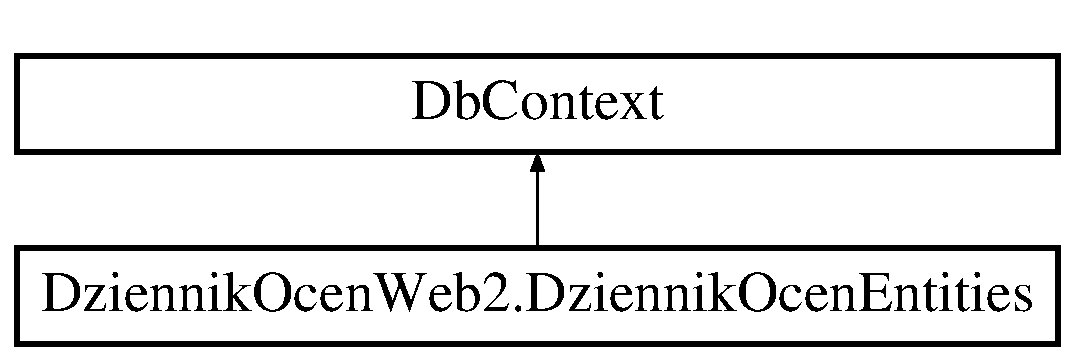
\includegraphics[height=2.000000cm]{class_dziennik_ocen_web2_1_1_dziennik_ocen_entities}
\end{center}
\end{figure}
\subsection*{Public Member Functions}
\begin{DoxyCompactItemize}
\item 
\hyperlink{class_dziennik_ocen_web2_1_1_dziennik_ocen_entities_a5fd581ca9a221a465221ee4b10229dc5}{Dziennik\+Ocen\+Entities} ()
\end{DoxyCompactItemize}
\subsection*{Protected Member Functions}
\begin{DoxyCompactItemize}
\item 
override void \hyperlink{class_dziennik_ocen_web2_1_1_dziennik_ocen_entities_a39a77c5c71b076abfb757275c435ddd5}{On\+Model\+Creating} (Db\+Model\+Builder model\+Builder)
\end{DoxyCompactItemize}
\subsection*{Properties}
\begin{DoxyCompactItemize}
\item 
Db\+Set$<$ \hyperlink{class_dziennik_ocen_web2_1_1_g_r_u_p_a}{G\+R\+U\+PA} $>$ \hyperlink{class_dziennik_ocen_web2_1_1_dziennik_ocen_entities_ab13ca42decd07b8192af9f6119bc59de}{G\+R\+U\+PA}\hspace{0.3cm}{\ttfamily  \mbox{[}get, set\mbox{]}}
\item 
Db\+Set$<$ \hyperlink{class_dziennik_ocen_web2_1_1_p_r_o_j_e_k_t}{P\+R\+O\+J\+E\+KT} $>$ \hyperlink{class_dziennik_ocen_web2_1_1_dziennik_ocen_entities_a54d68132f5c42eef109e851010e11da9}{P\+R\+O\+J\+E\+KT}\hspace{0.3cm}{\ttfamily  \mbox{[}get, set\mbox{]}}
\item 
Db\+Set$<$ \hyperlink{class_dziennik_ocen_web2_1_1projekty}{projekty} $>$ \hyperlink{class_dziennik_ocen_web2_1_1_dziennik_ocen_entities_aa3c51299884a923f965cb752327cb262}{projekty}\hspace{0.3cm}{\ttfamily  \mbox{[}get, set\mbox{]}}
\item 
Db\+Set$<$ \hyperlink{class_dziennik_ocen_web2_1_1_p_r_o_w_a_d_z_xC4_x84_c_y}{P\+R\+O\+W\+A\+D\+ZĄ\+CY} $>$ \hyperlink{class_dziennik_ocen_web2_1_1_dziennik_ocen_entities_a5a16ff31fa82dac4e34ef4b7567dc69f}{P\+R\+O\+W\+A\+D\+ZĄ\+CY}\hspace{0.3cm}{\ttfamily  \mbox{[}get, set\mbox{]}}
\item 
Db\+Set$<$ \hyperlink{class_dziennik_ocen_web2_1_1_p_r_z_e_d_m_i_o_t}{P\+R\+Z\+E\+D\+M\+I\+OT} $>$ \hyperlink{class_dziennik_ocen_web2_1_1_dziennik_ocen_entities_a88674504492aa9e05e74b2816501674f}{P\+R\+Z\+E\+D\+M\+I\+OT}\hspace{0.3cm}{\ttfamily  \mbox{[}get, set\mbox{]}}
\item 
Db\+Set$<$ \hyperlink{class_dziennik_ocen_web2_1_1przedmioty}{przedmioty} $>$ \hyperlink{class_dziennik_ocen_web2_1_1_dziennik_ocen_entities_ae46ef315cbd71e340160ce2f680479dd}{przedmioty}\hspace{0.3cm}{\ttfamily  \mbox{[}get, set\mbox{]}}
\item 
Db\+Set$<$ \hyperlink{class_dziennik_ocen_web2_1_1_s_t_u_d_e_n_t}{S\+T\+U\+D\+E\+NT} $>$ \hyperlink{class_dziennik_ocen_web2_1_1_dziennik_ocen_entities_ae6800c45c0cb8ea55ca7bb8a767d9763}{S\+T\+U\+D\+E\+NT}\hspace{0.3cm}{\ttfamily  \mbox{[}get, set\mbox{]}}
\end{DoxyCompactItemize}


\subsection{Constructor \& Destructor Documentation}
\mbox{\Hypertarget{class_dziennik_ocen_web2_1_1_dziennik_ocen_entities_a5fd581ca9a221a465221ee4b10229dc5}\label{class_dziennik_ocen_web2_1_1_dziennik_ocen_entities_a5fd581ca9a221a465221ee4b10229dc5}} 
\index{Dziennik\+Ocen\+Web2\+::\+Dziennik\+Ocen\+Entities@{Dziennik\+Ocen\+Web2\+::\+Dziennik\+Ocen\+Entities}!Dziennik\+Ocen\+Entities@{Dziennik\+Ocen\+Entities}}
\index{Dziennik\+Ocen\+Entities@{Dziennik\+Ocen\+Entities}!Dziennik\+Ocen\+Web2\+::\+Dziennik\+Ocen\+Entities@{Dziennik\+Ocen\+Web2\+::\+Dziennik\+Ocen\+Entities}}
\subsubsection{\texorpdfstring{Dziennik\+Ocen\+Entities()}{DziennikOcenEntities()}}
{\footnotesize\ttfamily Dziennik\+Ocen\+Web2.\+Dziennik\+Ocen\+Entities.\+Dziennik\+Ocen\+Entities (\begin{DoxyParamCaption}{ }\end{DoxyParamCaption})\hspace{0.3cm}{\ttfamily [inline]}}



\subsection{Member Function Documentation}
\mbox{\Hypertarget{class_dziennik_ocen_web2_1_1_dziennik_ocen_entities_a39a77c5c71b076abfb757275c435ddd5}\label{class_dziennik_ocen_web2_1_1_dziennik_ocen_entities_a39a77c5c71b076abfb757275c435ddd5}} 
\index{Dziennik\+Ocen\+Web2\+::\+Dziennik\+Ocen\+Entities@{Dziennik\+Ocen\+Web2\+::\+Dziennik\+Ocen\+Entities}!On\+Model\+Creating@{On\+Model\+Creating}}
\index{On\+Model\+Creating@{On\+Model\+Creating}!Dziennik\+Ocen\+Web2\+::\+Dziennik\+Ocen\+Entities@{Dziennik\+Ocen\+Web2\+::\+Dziennik\+Ocen\+Entities}}
\subsubsection{\texorpdfstring{On\+Model\+Creating()}{OnModelCreating()}}
{\footnotesize\ttfamily override void Dziennik\+Ocen\+Web2.\+Dziennik\+Ocen\+Entities.\+On\+Model\+Creating (\begin{DoxyParamCaption}\item[{Db\+Model\+Builder}]{model\+Builder }\end{DoxyParamCaption})\hspace{0.3cm}{\ttfamily [inline]}, {\ttfamily [protected]}}



\subsection{Property Documentation}
\mbox{\Hypertarget{class_dziennik_ocen_web2_1_1_dziennik_ocen_entities_ab13ca42decd07b8192af9f6119bc59de}\label{class_dziennik_ocen_web2_1_1_dziennik_ocen_entities_ab13ca42decd07b8192af9f6119bc59de}} 
\index{Dziennik\+Ocen\+Web2\+::\+Dziennik\+Ocen\+Entities@{Dziennik\+Ocen\+Web2\+::\+Dziennik\+Ocen\+Entities}!G\+R\+U\+PA@{G\+R\+U\+PA}}
\index{G\+R\+U\+PA@{G\+R\+U\+PA}!Dziennik\+Ocen\+Web2\+::\+Dziennik\+Ocen\+Entities@{Dziennik\+Ocen\+Web2\+::\+Dziennik\+Ocen\+Entities}}
\subsubsection{\texorpdfstring{G\+R\+U\+PA}{GRUPA}}
{\footnotesize\ttfamily Db\+Set$<$\hyperlink{class_dziennik_ocen_web2_1_1_g_r_u_p_a}{G\+R\+U\+PA}$>$ Dziennik\+Ocen\+Web2.\+Dziennik\+Ocen\+Entities.\+G\+R\+U\+PA\hspace{0.3cm}{\ttfamily [get]}, {\ttfamily [set]}}

\mbox{\Hypertarget{class_dziennik_ocen_web2_1_1_dziennik_ocen_entities_a54d68132f5c42eef109e851010e11da9}\label{class_dziennik_ocen_web2_1_1_dziennik_ocen_entities_a54d68132f5c42eef109e851010e11da9}} 
\index{Dziennik\+Ocen\+Web2\+::\+Dziennik\+Ocen\+Entities@{Dziennik\+Ocen\+Web2\+::\+Dziennik\+Ocen\+Entities}!P\+R\+O\+J\+E\+KT@{P\+R\+O\+J\+E\+KT}}
\index{P\+R\+O\+J\+E\+KT@{P\+R\+O\+J\+E\+KT}!Dziennik\+Ocen\+Web2\+::\+Dziennik\+Ocen\+Entities@{Dziennik\+Ocen\+Web2\+::\+Dziennik\+Ocen\+Entities}}
\subsubsection{\texorpdfstring{P\+R\+O\+J\+E\+KT}{PROJEKT}}
{\footnotesize\ttfamily Db\+Set$<$\hyperlink{class_dziennik_ocen_web2_1_1_p_r_o_j_e_k_t}{P\+R\+O\+J\+E\+KT}$>$ Dziennik\+Ocen\+Web2.\+Dziennik\+Ocen\+Entities.\+P\+R\+O\+J\+E\+KT\hspace{0.3cm}{\ttfamily [get]}, {\ttfamily [set]}}

\mbox{\Hypertarget{class_dziennik_ocen_web2_1_1_dziennik_ocen_entities_aa3c51299884a923f965cb752327cb262}\label{class_dziennik_ocen_web2_1_1_dziennik_ocen_entities_aa3c51299884a923f965cb752327cb262}} 
\index{Dziennik\+Ocen\+Web2\+::\+Dziennik\+Ocen\+Entities@{Dziennik\+Ocen\+Web2\+::\+Dziennik\+Ocen\+Entities}!projekty@{projekty}}
\index{projekty@{projekty}!Dziennik\+Ocen\+Web2\+::\+Dziennik\+Ocen\+Entities@{Dziennik\+Ocen\+Web2\+::\+Dziennik\+Ocen\+Entities}}
\subsubsection{\texorpdfstring{projekty}{projekty}}
{\footnotesize\ttfamily Db\+Set$<$\hyperlink{class_dziennik_ocen_web2_1_1projekty}{projekty}$>$ Dziennik\+Ocen\+Web2.\+Dziennik\+Ocen\+Entities.\+projekty\hspace{0.3cm}{\ttfamily [get]}, {\ttfamily [set]}}

\mbox{\Hypertarget{class_dziennik_ocen_web2_1_1_dziennik_ocen_entities_a5a16ff31fa82dac4e34ef4b7567dc69f}\label{class_dziennik_ocen_web2_1_1_dziennik_ocen_entities_a5a16ff31fa82dac4e34ef4b7567dc69f}} 
\index{Dziennik\+Ocen\+Web2\+::\+Dziennik\+Ocen\+Entities@{Dziennik\+Ocen\+Web2\+::\+Dziennik\+Ocen\+Entities}!P\+R\+O\+W\+A\+D\+ZĄ\+CY@{P\+R\+O\+W\+A\+D\+ZĄ\+CY}}
\index{P\+R\+O\+W\+A\+D\+ZĄ\+CY@{P\+R\+O\+W\+A\+D\+ZĄ\+CY}!Dziennik\+Ocen\+Web2\+::\+Dziennik\+Ocen\+Entities@{Dziennik\+Ocen\+Web2\+::\+Dziennik\+Ocen\+Entities}}
\subsubsection{\texorpdfstring{P\+R\+O\+W\+A\+D\+ZĄ\+CY}{PROWADZĄCY}}
{\footnotesize\ttfamily Db\+Set$<$\hyperlink{class_dziennik_ocen_web2_1_1_p_r_o_w_a_d_z_xC4_x84_c_y}{P\+R\+O\+W\+A\+D\+ZĄ\+CY}$>$ Dziennik\+Ocen\+Web2.\+Dziennik\+Ocen\+Entities.\+P\+R\+O\+W\+A\+D\+ZĄ\+CY\hspace{0.3cm}{\ttfamily [get]}, {\ttfamily [set]}}

\mbox{\Hypertarget{class_dziennik_ocen_web2_1_1_dziennik_ocen_entities_a88674504492aa9e05e74b2816501674f}\label{class_dziennik_ocen_web2_1_1_dziennik_ocen_entities_a88674504492aa9e05e74b2816501674f}} 
\index{Dziennik\+Ocen\+Web2\+::\+Dziennik\+Ocen\+Entities@{Dziennik\+Ocen\+Web2\+::\+Dziennik\+Ocen\+Entities}!P\+R\+Z\+E\+D\+M\+I\+OT@{P\+R\+Z\+E\+D\+M\+I\+OT}}
\index{P\+R\+Z\+E\+D\+M\+I\+OT@{P\+R\+Z\+E\+D\+M\+I\+OT}!Dziennik\+Ocen\+Web2\+::\+Dziennik\+Ocen\+Entities@{Dziennik\+Ocen\+Web2\+::\+Dziennik\+Ocen\+Entities}}
\subsubsection{\texorpdfstring{P\+R\+Z\+E\+D\+M\+I\+OT}{PRZEDMIOT}}
{\footnotesize\ttfamily Db\+Set$<$\hyperlink{class_dziennik_ocen_web2_1_1_p_r_z_e_d_m_i_o_t}{P\+R\+Z\+E\+D\+M\+I\+OT}$>$ Dziennik\+Ocen\+Web2.\+Dziennik\+Ocen\+Entities.\+P\+R\+Z\+E\+D\+M\+I\+OT\hspace{0.3cm}{\ttfamily [get]}, {\ttfamily [set]}}

\mbox{\Hypertarget{class_dziennik_ocen_web2_1_1_dziennik_ocen_entities_ae46ef315cbd71e340160ce2f680479dd}\label{class_dziennik_ocen_web2_1_1_dziennik_ocen_entities_ae46ef315cbd71e340160ce2f680479dd}} 
\index{Dziennik\+Ocen\+Web2\+::\+Dziennik\+Ocen\+Entities@{Dziennik\+Ocen\+Web2\+::\+Dziennik\+Ocen\+Entities}!przedmioty@{przedmioty}}
\index{przedmioty@{przedmioty}!Dziennik\+Ocen\+Web2\+::\+Dziennik\+Ocen\+Entities@{Dziennik\+Ocen\+Web2\+::\+Dziennik\+Ocen\+Entities}}
\subsubsection{\texorpdfstring{przedmioty}{przedmioty}}
{\footnotesize\ttfamily Db\+Set$<$\hyperlink{class_dziennik_ocen_web2_1_1przedmioty}{przedmioty}$>$ Dziennik\+Ocen\+Web2.\+Dziennik\+Ocen\+Entities.\+przedmioty\hspace{0.3cm}{\ttfamily [get]}, {\ttfamily [set]}}

\mbox{\Hypertarget{class_dziennik_ocen_web2_1_1_dziennik_ocen_entities_ae6800c45c0cb8ea55ca7bb8a767d9763}\label{class_dziennik_ocen_web2_1_1_dziennik_ocen_entities_ae6800c45c0cb8ea55ca7bb8a767d9763}} 
\index{Dziennik\+Ocen\+Web2\+::\+Dziennik\+Ocen\+Entities@{Dziennik\+Ocen\+Web2\+::\+Dziennik\+Ocen\+Entities}!S\+T\+U\+D\+E\+NT@{S\+T\+U\+D\+E\+NT}}
\index{S\+T\+U\+D\+E\+NT@{S\+T\+U\+D\+E\+NT}!Dziennik\+Ocen\+Web2\+::\+Dziennik\+Ocen\+Entities@{Dziennik\+Ocen\+Web2\+::\+Dziennik\+Ocen\+Entities}}
\subsubsection{\texorpdfstring{S\+T\+U\+D\+E\+NT}{STUDENT}}
{\footnotesize\ttfamily Db\+Set$<$\hyperlink{class_dziennik_ocen_web2_1_1_s_t_u_d_e_n_t}{S\+T\+U\+D\+E\+NT}$>$ Dziennik\+Ocen\+Web2.\+Dziennik\+Ocen\+Entities.\+S\+T\+U\+D\+E\+NT\hspace{0.3cm}{\ttfamily [get]}, {\ttfamily [set]}}



The documentation for this class was generated from the following file\+:\begin{DoxyCompactItemize}
\item 
Dziennik\+Ocen\+Web2/\hyperlink{_dziennik_ocen_web_model_8_context_8cs}{Dziennik\+Ocen\+Web\+Model.\+Context.\+cs}\end{DoxyCompactItemize}

\hypertarget{class_dziennik_ocen_web2_1_1_global}{}\section{Dziennik\+Ocen\+Web2.\+Global Class Reference}
\label{class_dziennik_ocen_web2_1_1_global}\index{Dziennik\+Ocen\+Web2.\+Global@{Dziennik\+Ocen\+Web2.\+Global}}
Inheritance diagram for Dziennik\+Ocen\+Web2.\+Global\+:\begin{figure}[H]
\begin{center}
\leavevmode
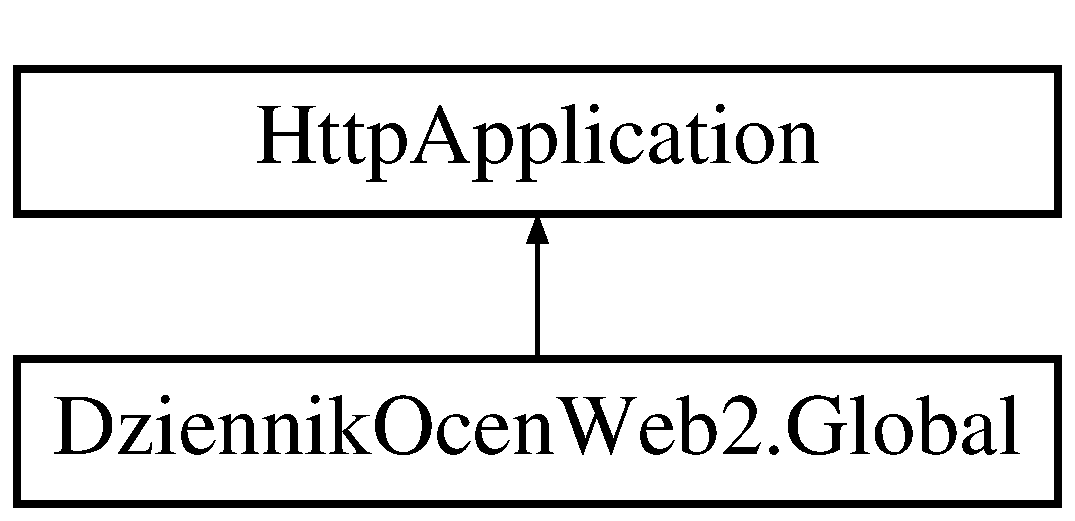
\includegraphics[height=2.000000cm]{class_dziennik_ocen_web2_1_1_global}
\end{center}
\end{figure}
\subsection*{Protected Member Functions}
\begin{DoxyCompactItemize}
\item 
void \hyperlink{class_dziennik_ocen_web2_1_1_global_a8c54a9bf2279bed6da81321977d82574}{Application\+\_\+\+Start} (object sender, Event\+Args e)
\end{DoxyCompactItemize}


\subsection{Member Function Documentation}
\mbox{\Hypertarget{class_dziennik_ocen_web2_1_1_global_a8c54a9bf2279bed6da81321977d82574}\label{class_dziennik_ocen_web2_1_1_global_a8c54a9bf2279bed6da81321977d82574}} 
\index{Dziennik\+Ocen\+Web2\+::\+Global@{Dziennik\+Ocen\+Web2\+::\+Global}!Application\+\_\+\+Start@{Application\+\_\+\+Start}}
\index{Application\+\_\+\+Start@{Application\+\_\+\+Start}!Dziennik\+Ocen\+Web2\+::\+Global@{Dziennik\+Ocen\+Web2\+::\+Global}}
\subsubsection{\texorpdfstring{Application\+\_\+\+Start()}{Application\_Start()}}
{\footnotesize\ttfamily void Dziennik\+Ocen\+Web2.\+Global.\+Application\+\_\+\+Start (\begin{DoxyParamCaption}\item[{object}]{sender,  }\item[{Event\+Args}]{e }\end{DoxyParamCaption})\hspace{0.3cm}{\ttfamily [inline]}, {\ttfamily [protected]}}



The documentation for this class was generated from the following file\+:\begin{DoxyCompactItemize}
\item 
Dziennik\+Ocen\+Web2/\hyperlink{_global_8asax_8cs}{Global.\+asax.\+cs}\end{DoxyCompactItemize}

\hypertarget{class_dziennik_ocen_web2_1_1_g_r_u_p_a}{}\section{Dziennik\+Ocen\+Web2.\+G\+R\+U\+PA Class Reference}
\label{class_dziennik_ocen_web2_1_1_g_r_u_p_a}\index{Dziennik\+Ocen\+Web2.\+G\+R\+U\+PA@{Dziennik\+Ocen\+Web2.\+G\+R\+U\+PA}}
\subsection*{Public Member Functions}
\begin{DoxyCompactItemize}
\item 
\hyperlink{class_dziennik_ocen_web2_1_1_g_r_u_p_a_a59d87f0cb1bf4e2be67c497c37ed28b1}{G\+R\+U\+PA} ()
\end{DoxyCompactItemize}
\subsection*{Properties}
\begin{DoxyCompactItemize}
\item 
int \hyperlink{class_dziennik_ocen_web2_1_1_g_r_u_p_a_a88256b43c28c202822d84e0e2ca61eb0}{id\+\_\+\+G\+R\+U\+PY}\hspace{0.3cm}{\ttfamily  \mbox{[}get, set\mbox{]}}
\item 
string \hyperlink{class_dziennik_ocen_web2_1_1_g_r_u_p_a_aea3a7c3d2aa3820ec24bd079a8823dbd}{nazwa\+\_\+grupy}\hspace{0.3cm}{\ttfamily  \mbox{[}get, set\mbox{]}}
\item 
virtual I\+Collection$<$ \hyperlink{class_dziennik_ocen_web2_1_1_s_t_u_d_e_n_t}{S\+T\+U\+D\+E\+NT} $>$ \hyperlink{class_dziennik_ocen_web2_1_1_g_r_u_p_a_a5814085ba05380474ab502665b53df0a}{S\+T\+U\+D\+E\+NT}\hspace{0.3cm}{\ttfamily  \mbox{[}get, set\mbox{]}}
\end{DoxyCompactItemize}


\subsection{Constructor \& Destructor Documentation}
\mbox{\Hypertarget{class_dziennik_ocen_web2_1_1_g_r_u_p_a_a59d87f0cb1bf4e2be67c497c37ed28b1}\label{class_dziennik_ocen_web2_1_1_g_r_u_p_a_a59d87f0cb1bf4e2be67c497c37ed28b1}} 
\index{Dziennik\+Ocen\+Web2\+::\+G\+R\+U\+PA@{Dziennik\+Ocen\+Web2\+::\+G\+R\+U\+PA}!G\+R\+U\+PA@{G\+R\+U\+PA}}
\index{G\+R\+U\+PA@{G\+R\+U\+PA}!Dziennik\+Ocen\+Web2\+::\+G\+R\+U\+PA@{Dziennik\+Ocen\+Web2\+::\+G\+R\+U\+PA}}
\subsubsection{\texorpdfstring{G\+R\+U\+P\+A()}{GRUPA()}}
{\footnotesize\ttfamily Dziennik\+Ocen\+Web2.\+G\+R\+U\+P\+A.\+G\+R\+U\+PA (\begin{DoxyParamCaption}{ }\end{DoxyParamCaption})\hspace{0.3cm}{\ttfamily [inline]}}



\subsection{Property Documentation}
\mbox{\Hypertarget{class_dziennik_ocen_web2_1_1_g_r_u_p_a_a88256b43c28c202822d84e0e2ca61eb0}\label{class_dziennik_ocen_web2_1_1_g_r_u_p_a_a88256b43c28c202822d84e0e2ca61eb0}} 
\index{Dziennik\+Ocen\+Web2\+::\+G\+R\+U\+PA@{Dziennik\+Ocen\+Web2\+::\+G\+R\+U\+PA}!id\+\_\+\+G\+R\+U\+PY@{id\+\_\+\+G\+R\+U\+PY}}
\index{id\+\_\+\+G\+R\+U\+PY@{id\+\_\+\+G\+R\+U\+PY}!Dziennik\+Ocen\+Web2\+::\+G\+R\+U\+PA@{Dziennik\+Ocen\+Web2\+::\+G\+R\+U\+PA}}
\subsubsection{\texorpdfstring{id\+\_\+\+G\+R\+U\+PY}{id\_GRUPY}}
{\footnotesize\ttfamily int Dziennik\+Ocen\+Web2.\+G\+R\+U\+P\+A.\+id\+\_\+\+G\+R\+U\+PY\hspace{0.3cm}{\ttfamily [get]}, {\ttfamily [set]}}

\mbox{\Hypertarget{class_dziennik_ocen_web2_1_1_g_r_u_p_a_aea3a7c3d2aa3820ec24bd079a8823dbd}\label{class_dziennik_ocen_web2_1_1_g_r_u_p_a_aea3a7c3d2aa3820ec24bd079a8823dbd}} 
\index{Dziennik\+Ocen\+Web2\+::\+G\+R\+U\+PA@{Dziennik\+Ocen\+Web2\+::\+G\+R\+U\+PA}!nazwa\+\_\+grupy@{nazwa\+\_\+grupy}}
\index{nazwa\+\_\+grupy@{nazwa\+\_\+grupy}!Dziennik\+Ocen\+Web2\+::\+G\+R\+U\+PA@{Dziennik\+Ocen\+Web2\+::\+G\+R\+U\+PA}}
\subsubsection{\texorpdfstring{nazwa\+\_\+grupy}{nazwa\_grupy}}
{\footnotesize\ttfamily string Dziennik\+Ocen\+Web2.\+G\+R\+U\+P\+A.\+nazwa\+\_\+grupy\hspace{0.3cm}{\ttfamily [get]}, {\ttfamily [set]}}

\mbox{\Hypertarget{class_dziennik_ocen_web2_1_1_g_r_u_p_a_a5814085ba05380474ab502665b53df0a}\label{class_dziennik_ocen_web2_1_1_g_r_u_p_a_a5814085ba05380474ab502665b53df0a}} 
\index{Dziennik\+Ocen\+Web2\+::\+G\+R\+U\+PA@{Dziennik\+Ocen\+Web2\+::\+G\+R\+U\+PA}!S\+T\+U\+D\+E\+NT@{S\+T\+U\+D\+E\+NT}}
\index{S\+T\+U\+D\+E\+NT@{S\+T\+U\+D\+E\+NT}!Dziennik\+Ocen\+Web2\+::\+G\+R\+U\+PA@{Dziennik\+Ocen\+Web2\+::\+G\+R\+U\+PA}}
\subsubsection{\texorpdfstring{S\+T\+U\+D\+E\+NT}{STUDENT}}
{\footnotesize\ttfamily virtual I\+Collection$<$\hyperlink{class_dziennik_ocen_web2_1_1_s_t_u_d_e_n_t}{S\+T\+U\+D\+E\+NT}$>$ Dziennik\+Ocen\+Web2.\+G\+R\+U\+P\+A.\+S\+T\+U\+D\+E\+NT\hspace{0.3cm}{\ttfamily [get]}, {\ttfamily [set]}}



The documentation for this class was generated from the following file\+:\begin{DoxyCompactItemize}
\item 
Dziennik\+Ocen\+Web2/\hyperlink{_g_r_u_p_a_8cs}{G\+R\+U\+P\+A.\+cs}\end{DoxyCompactItemize}

\hypertarget{class_dziennik_ocen_web2_1_1_p_r_o_j_e_k_t}{}\section{Dziennik\+Ocen\+Web2.\+P\+R\+O\+J\+E\+KT Class Reference}
\label{class_dziennik_ocen_web2_1_1_p_r_o_j_e_k_t}\index{Dziennik\+Ocen\+Web2.\+P\+R\+O\+J\+E\+KT@{Dziennik\+Ocen\+Web2.\+P\+R\+O\+J\+E\+KT}}
\subsection*{Public Member Functions}
\begin{DoxyCompactItemize}
\item 
\hyperlink{class_dziennik_ocen_web2_1_1_p_r_o_j_e_k_t_a75c1a0773b2350ed7341d6b1089ced90}{P\+R\+O\+J\+E\+KT} ()
\end{DoxyCompactItemize}
\subsection*{Properties}
\begin{DoxyCompactItemize}
\item 
int \hyperlink{class_dziennik_ocen_web2_1_1_p_r_o_j_e_k_t_abb785d4a4041798f2821f83c77497032}{id\+\_\+\+P\+R\+O\+J\+E\+K\+TU}\hspace{0.3cm}{\ttfamily  \mbox{[}get, set\mbox{]}}
\item 
Nullable$<$ int $>$ \hyperlink{class_dziennik_ocen_web2_1_1_p_r_o_j_e_k_t_a5d1013fc6420908499195821e393864a}{id\+\_\+\+P\+R\+Z\+E\+D\+M\+I\+O\+TU}\hspace{0.3cm}{\ttfamily  \mbox{[}get, set\mbox{]}}
\item 
string \hyperlink{class_dziennik_ocen_web2_1_1_p_r_o_j_e_k_t_a2ecf2225caa21996453cc82110bef760}{nazwa\+\_\+projektu}\hspace{0.3cm}{\ttfamily  \mbox{[}get, set\mbox{]}}
\item 
string \hyperlink{class_dziennik_ocen_web2_1_1_p_r_o_j_e_k_t_aa221ed522d380620586a91300738d0cc}{opis\+\_\+projektu}\hspace{0.3cm}{\ttfamily  \mbox{[}get, set\mbox{]}}
\item 
virtual \hyperlink{class_dziennik_ocen_web2_1_1_p_r_z_e_d_m_i_o_t}{P\+R\+Z\+E\+D\+M\+I\+OT} \hyperlink{class_dziennik_ocen_web2_1_1_p_r_o_j_e_k_t_aa9a826689c26127e29cc455b9cd9518d}{P\+R\+Z\+E\+D\+M\+I\+OT}\hspace{0.3cm}{\ttfamily  \mbox{[}get, set\mbox{]}}
\item 
virtual I\+Collection$<$ \hyperlink{class_dziennik_ocen_web2_1_1projekty}{projekty} $>$ \hyperlink{class_dziennik_ocen_web2_1_1_p_r_o_j_e_k_t_afb3ac65ee2f14cc791decb4b8828210a}{projekty}\hspace{0.3cm}{\ttfamily  \mbox{[}get, set\mbox{]}}
\end{DoxyCompactItemize}


\subsection{Constructor \& Destructor Documentation}
\mbox{\Hypertarget{class_dziennik_ocen_web2_1_1_p_r_o_j_e_k_t_a75c1a0773b2350ed7341d6b1089ced90}\label{class_dziennik_ocen_web2_1_1_p_r_o_j_e_k_t_a75c1a0773b2350ed7341d6b1089ced90}} 
\index{Dziennik\+Ocen\+Web2\+::\+P\+R\+O\+J\+E\+KT@{Dziennik\+Ocen\+Web2\+::\+P\+R\+O\+J\+E\+KT}!P\+R\+O\+J\+E\+KT@{P\+R\+O\+J\+E\+KT}}
\index{P\+R\+O\+J\+E\+KT@{P\+R\+O\+J\+E\+KT}!Dziennik\+Ocen\+Web2\+::\+P\+R\+O\+J\+E\+KT@{Dziennik\+Ocen\+Web2\+::\+P\+R\+O\+J\+E\+KT}}
\subsubsection{\texorpdfstring{P\+R\+O\+J\+E\+K\+T()}{PROJEKT()}}
{\footnotesize\ttfamily Dziennik\+Ocen\+Web2.\+P\+R\+O\+J\+E\+K\+T.\+P\+R\+O\+J\+E\+KT (\begin{DoxyParamCaption}{ }\end{DoxyParamCaption})\hspace{0.3cm}{\ttfamily [inline]}}



\subsection{Property Documentation}
\mbox{\Hypertarget{class_dziennik_ocen_web2_1_1_p_r_o_j_e_k_t_abb785d4a4041798f2821f83c77497032}\label{class_dziennik_ocen_web2_1_1_p_r_o_j_e_k_t_abb785d4a4041798f2821f83c77497032}} 
\index{Dziennik\+Ocen\+Web2\+::\+P\+R\+O\+J\+E\+KT@{Dziennik\+Ocen\+Web2\+::\+P\+R\+O\+J\+E\+KT}!id\+\_\+\+P\+R\+O\+J\+E\+K\+TU@{id\+\_\+\+P\+R\+O\+J\+E\+K\+TU}}
\index{id\+\_\+\+P\+R\+O\+J\+E\+K\+TU@{id\+\_\+\+P\+R\+O\+J\+E\+K\+TU}!Dziennik\+Ocen\+Web2\+::\+P\+R\+O\+J\+E\+KT@{Dziennik\+Ocen\+Web2\+::\+P\+R\+O\+J\+E\+KT}}
\subsubsection{\texorpdfstring{id\+\_\+\+P\+R\+O\+J\+E\+K\+TU}{id\_PROJEKTU}}
{\footnotesize\ttfamily int Dziennik\+Ocen\+Web2.\+P\+R\+O\+J\+E\+K\+T.\+id\+\_\+\+P\+R\+O\+J\+E\+K\+TU\hspace{0.3cm}{\ttfamily [get]}, {\ttfamily [set]}}

\mbox{\Hypertarget{class_dziennik_ocen_web2_1_1_p_r_o_j_e_k_t_a5d1013fc6420908499195821e393864a}\label{class_dziennik_ocen_web2_1_1_p_r_o_j_e_k_t_a5d1013fc6420908499195821e393864a}} 
\index{Dziennik\+Ocen\+Web2\+::\+P\+R\+O\+J\+E\+KT@{Dziennik\+Ocen\+Web2\+::\+P\+R\+O\+J\+E\+KT}!id\+\_\+\+P\+R\+Z\+E\+D\+M\+I\+O\+TU@{id\+\_\+\+P\+R\+Z\+E\+D\+M\+I\+O\+TU}}
\index{id\+\_\+\+P\+R\+Z\+E\+D\+M\+I\+O\+TU@{id\+\_\+\+P\+R\+Z\+E\+D\+M\+I\+O\+TU}!Dziennik\+Ocen\+Web2\+::\+P\+R\+O\+J\+E\+KT@{Dziennik\+Ocen\+Web2\+::\+P\+R\+O\+J\+E\+KT}}
\subsubsection{\texorpdfstring{id\+\_\+\+P\+R\+Z\+E\+D\+M\+I\+O\+TU}{id\_PRZEDMIOTU}}
{\footnotesize\ttfamily Nullable$<$int$>$ Dziennik\+Ocen\+Web2.\+P\+R\+O\+J\+E\+K\+T.\+id\+\_\+\+P\+R\+Z\+E\+D\+M\+I\+O\+TU\hspace{0.3cm}{\ttfamily [get]}, {\ttfamily [set]}}

\mbox{\Hypertarget{class_dziennik_ocen_web2_1_1_p_r_o_j_e_k_t_a2ecf2225caa21996453cc82110bef760}\label{class_dziennik_ocen_web2_1_1_p_r_o_j_e_k_t_a2ecf2225caa21996453cc82110bef760}} 
\index{Dziennik\+Ocen\+Web2\+::\+P\+R\+O\+J\+E\+KT@{Dziennik\+Ocen\+Web2\+::\+P\+R\+O\+J\+E\+KT}!nazwa\+\_\+projektu@{nazwa\+\_\+projektu}}
\index{nazwa\+\_\+projektu@{nazwa\+\_\+projektu}!Dziennik\+Ocen\+Web2\+::\+P\+R\+O\+J\+E\+KT@{Dziennik\+Ocen\+Web2\+::\+P\+R\+O\+J\+E\+KT}}
\subsubsection{\texorpdfstring{nazwa\+\_\+projektu}{nazwa\_projektu}}
{\footnotesize\ttfamily string Dziennik\+Ocen\+Web2.\+P\+R\+O\+J\+E\+K\+T.\+nazwa\+\_\+projektu\hspace{0.3cm}{\ttfamily [get]}, {\ttfamily [set]}}

\mbox{\Hypertarget{class_dziennik_ocen_web2_1_1_p_r_o_j_e_k_t_aa221ed522d380620586a91300738d0cc}\label{class_dziennik_ocen_web2_1_1_p_r_o_j_e_k_t_aa221ed522d380620586a91300738d0cc}} 
\index{Dziennik\+Ocen\+Web2\+::\+P\+R\+O\+J\+E\+KT@{Dziennik\+Ocen\+Web2\+::\+P\+R\+O\+J\+E\+KT}!opis\+\_\+projektu@{opis\+\_\+projektu}}
\index{opis\+\_\+projektu@{opis\+\_\+projektu}!Dziennik\+Ocen\+Web2\+::\+P\+R\+O\+J\+E\+KT@{Dziennik\+Ocen\+Web2\+::\+P\+R\+O\+J\+E\+KT}}
\subsubsection{\texorpdfstring{opis\+\_\+projektu}{opis\_projektu}}
{\footnotesize\ttfamily string Dziennik\+Ocen\+Web2.\+P\+R\+O\+J\+E\+K\+T.\+opis\+\_\+projektu\hspace{0.3cm}{\ttfamily [get]}, {\ttfamily [set]}}

\mbox{\Hypertarget{class_dziennik_ocen_web2_1_1_p_r_o_j_e_k_t_afb3ac65ee2f14cc791decb4b8828210a}\label{class_dziennik_ocen_web2_1_1_p_r_o_j_e_k_t_afb3ac65ee2f14cc791decb4b8828210a}} 
\index{Dziennik\+Ocen\+Web2\+::\+P\+R\+O\+J\+E\+KT@{Dziennik\+Ocen\+Web2\+::\+P\+R\+O\+J\+E\+KT}!projekty@{projekty}}
\index{projekty@{projekty}!Dziennik\+Ocen\+Web2\+::\+P\+R\+O\+J\+E\+KT@{Dziennik\+Ocen\+Web2\+::\+P\+R\+O\+J\+E\+KT}}
\subsubsection{\texorpdfstring{projekty}{projekty}}
{\footnotesize\ttfamily virtual I\+Collection$<$\hyperlink{class_dziennik_ocen_web2_1_1projekty}{projekty}$>$ Dziennik\+Ocen\+Web2.\+P\+R\+O\+J\+E\+K\+T.\+projekty\hspace{0.3cm}{\ttfamily [get]}, {\ttfamily [set]}}

\mbox{\Hypertarget{class_dziennik_ocen_web2_1_1_p_r_o_j_e_k_t_aa9a826689c26127e29cc455b9cd9518d}\label{class_dziennik_ocen_web2_1_1_p_r_o_j_e_k_t_aa9a826689c26127e29cc455b9cd9518d}} 
\index{Dziennik\+Ocen\+Web2\+::\+P\+R\+O\+J\+E\+KT@{Dziennik\+Ocen\+Web2\+::\+P\+R\+O\+J\+E\+KT}!P\+R\+Z\+E\+D\+M\+I\+OT@{P\+R\+Z\+E\+D\+M\+I\+OT}}
\index{P\+R\+Z\+E\+D\+M\+I\+OT@{P\+R\+Z\+E\+D\+M\+I\+OT}!Dziennik\+Ocen\+Web2\+::\+P\+R\+O\+J\+E\+KT@{Dziennik\+Ocen\+Web2\+::\+P\+R\+O\+J\+E\+KT}}
\subsubsection{\texorpdfstring{P\+R\+Z\+E\+D\+M\+I\+OT}{PRZEDMIOT}}
{\footnotesize\ttfamily virtual \hyperlink{class_dziennik_ocen_web2_1_1_p_r_z_e_d_m_i_o_t}{P\+R\+Z\+E\+D\+M\+I\+OT} Dziennik\+Ocen\+Web2.\+P\+R\+O\+J\+E\+K\+T.\+P\+R\+Z\+E\+D\+M\+I\+OT\hspace{0.3cm}{\ttfamily [get]}, {\ttfamily [set]}}



The documentation for this class was generated from the following file\+:\begin{DoxyCompactItemize}
\item 
Dziennik\+Ocen\+Web2/\hyperlink{_p_r_o_j_e_k_t_8cs}{P\+R\+O\+J\+E\+K\+T.\+cs}\end{DoxyCompactItemize}

\hypertarget{class_dziennik_ocen_web2_1_1projekty}{}\section{Dziennik\+Ocen\+Web2.\+projekty Class Reference}
\label{class_dziennik_ocen_web2_1_1projekty}\index{Dziennik\+Ocen\+Web2.\+projekty@{Dziennik\+Ocen\+Web2.\+projekty}}
\subsection*{Properties}
\begin{DoxyCompactItemize}
\item 
int \hyperlink{class_dziennik_ocen_web2_1_1projekty_a358bd2a6d48327377151ff9f3c76b18f}{id\+\_\+\+S\+T\+U\+D\+E\+N\+TA}\hspace{0.3cm}{\ttfamily  \mbox{[}get, set\mbox{]}}
\item 
int \hyperlink{class_dziennik_ocen_web2_1_1projekty_a4852de59c6fd809bba01a6369f692b50}{id\+\_\+\+P\+R\+O\+J\+E\+K\+TU}\hspace{0.3cm}{\ttfamily  \mbox{[}get, set\mbox{]}}
\item 
int \hyperlink{class_dziennik_ocen_web2_1_1projekty_a7a6a4540f13cbfbeadee76e9b8cb9bcb}{id\+\_\+\+P\+R\+O\+W\+A\+D\+ZĄ\+C\+E\+GO}\hspace{0.3cm}{\ttfamily  \mbox{[}get, set\mbox{]}}
\item 
Nullable$<$ int $>$ \hyperlink{class_dziennik_ocen_web2_1_1projekty_a5b1edf2beb2bd5e452d354deabf48925}{ocena\+\_\+projektu}\hspace{0.3cm}{\ttfamily  \mbox{[}get, set\mbox{]}}
\item 
Nullable$<$ System.\+Date\+Time $>$ \hyperlink{class_dziennik_ocen_web2_1_1projekty_ab62a96d30e9d808b957532668bfb87a6}{data\+\_\+projektu}\hspace{0.3cm}{\ttfamily  \mbox{[}get, set\mbox{]}}
\item 
string \hyperlink{class_dziennik_ocen_web2_1_1projekty_a471cababa1b0fbb4e6cda43493f72bc8}{uwagi\+\_\+projektu}\hspace{0.3cm}{\ttfamily  \mbox{[}get, set\mbox{]}}
\item 
virtual \hyperlink{class_dziennik_ocen_web2_1_1_p_r_o_j_e_k_t}{P\+R\+O\+J\+E\+KT} \hyperlink{class_dziennik_ocen_web2_1_1projekty_ac665b7ca0ca45bd06976e7391c715a59}{P\+R\+O\+J\+E\+KT}\hspace{0.3cm}{\ttfamily  \mbox{[}get, set\mbox{]}}
\item 
virtual \hyperlink{class_dziennik_ocen_web2_1_1_p_r_o_w_a_d_z_xC4_x84_c_y}{P\+R\+O\+W\+A\+D\+ZĄ\+CY} \hyperlink{class_dziennik_ocen_web2_1_1projekty_a61cf4f0d0ea11f9a579a5d49404a3bc8}{P\+R\+O\+W\+A\+D\+ZĄ\+CY}\hspace{0.3cm}{\ttfamily  \mbox{[}get, set\mbox{]}}
\item 
virtual \hyperlink{class_dziennik_ocen_web2_1_1_s_t_u_d_e_n_t}{S\+T\+U\+D\+E\+NT} \hyperlink{class_dziennik_ocen_web2_1_1projekty_aa5da6dee04231489165719c3b7a2dec9}{S\+T\+U\+D\+E\+NT}\hspace{0.3cm}{\ttfamily  \mbox{[}get, set\mbox{]}}
\end{DoxyCompactItemize}


\subsection{Property Documentation}
\mbox{\Hypertarget{class_dziennik_ocen_web2_1_1projekty_ab62a96d30e9d808b957532668bfb87a6}\label{class_dziennik_ocen_web2_1_1projekty_ab62a96d30e9d808b957532668bfb87a6}} 
\index{Dziennik\+Ocen\+Web2\+::projekty@{Dziennik\+Ocen\+Web2\+::projekty}!data\+\_\+projektu@{data\+\_\+projektu}}
\index{data\+\_\+projektu@{data\+\_\+projektu}!Dziennik\+Ocen\+Web2\+::projekty@{Dziennik\+Ocen\+Web2\+::projekty}}
\subsubsection{\texorpdfstring{data\+\_\+projektu}{data\_projektu}}
{\footnotesize\ttfamily Nullable$<$System.\+Date\+Time$>$ Dziennik\+Ocen\+Web2.\+projekty.\+data\+\_\+projektu\hspace{0.3cm}{\ttfamily [get]}, {\ttfamily [set]}}

\mbox{\Hypertarget{class_dziennik_ocen_web2_1_1projekty_a4852de59c6fd809bba01a6369f692b50}\label{class_dziennik_ocen_web2_1_1projekty_a4852de59c6fd809bba01a6369f692b50}} 
\index{Dziennik\+Ocen\+Web2\+::projekty@{Dziennik\+Ocen\+Web2\+::projekty}!id\+\_\+\+P\+R\+O\+J\+E\+K\+TU@{id\+\_\+\+P\+R\+O\+J\+E\+K\+TU}}
\index{id\+\_\+\+P\+R\+O\+J\+E\+K\+TU@{id\+\_\+\+P\+R\+O\+J\+E\+K\+TU}!Dziennik\+Ocen\+Web2\+::projekty@{Dziennik\+Ocen\+Web2\+::projekty}}
\subsubsection{\texorpdfstring{id\+\_\+\+P\+R\+O\+J\+E\+K\+TU}{id\_PROJEKTU}}
{\footnotesize\ttfamily int Dziennik\+Ocen\+Web2.\+projekty.\+id\+\_\+\+P\+R\+O\+J\+E\+K\+TU\hspace{0.3cm}{\ttfamily [get]}, {\ttfamily [set]}}

\mbox{\Hypertarget{class_dziennik_ocen_web2_1_1projekty_a7a6a4540f13cbfbeadee76e9b8cb9bcb}\label{class_dziennik_ocen_web2_1_1projekty_a7a6a4540f13cbfbeadee76e9b8cb9bcb}} 
\index{Dziennik\+Ocen\+Web2\+::projekty@{Dziennik\+Ocen\+Web2\+::projekty}!id\+\_\+\+P\+R\+O\+W\+A\+D\+ZĄ\+C\+E\+GO@{id\+\_\+\+P\+R\+O\+W\+A\+D\+ZĄ\+C\+E\+GO}}
\index{id\+\_\+\+P\+R\+O\+W\+A\+D\+ZĄ\+C\+E\+GO@{id\+\_\+\+P\+R\+O\+W\+A\+D\+ZĄ\+C\+E\+GO}!Dziennik\+Ocen\+Web2\+::projekty@{Dziennik\+Ocen\+Web2\+::projekty}}
\subsubsection{\texorpdfstring{id\+\_\+\+P\+R\+O\+W\+A\+D\+ZĄ\+C\+E\+GO}{id\_PROWADZĄCEGO}}
{\footnotesize\ttfamily int Dziennik\+Ocen\+Web2.\+projekty.\+id\+\_\+\+P\+R\+O\+W\+A\+D\+ZĄ\+C\+E\+GO\hspace{0.3cm}{\ttfamily [get]}, {\ttfamily [set]}}

\mbox{\Hypertarget{class_dziennik_ocen_web2_1_1projekty_a358bd2a6d48327377151ff9f3c76b18f}\label{class_dziennik_ocen_web2_1_1projekty_a358bd2a6d48327377151ff9f3c76b18f}} 
\index{Dziennik\+Ocen\+Web2\+::projekty@{Dziennik\+Ocen\+Web2\+::projekty}!id\+\_\+\+S\+T\+U\+D\+E\+N\+TA@{id\+\_\+\+S\+T\+U\+D\+E\+N\+TA}}
\index{id\+\_\+\+S\+T\+U\+D\+E\+N\+TA@{id\+\_\+\+S\+T\+U\+D\+E\+N\+TA}!Dziennik\+Ocen\+Web2\+::projekty@{Dziennik\+Ocen\+Web2\+::projekty}}
\subsubsection{\texorpdfstring{id\+\_\+\+S\+T\+U\+D\+E\+N\+TA}{id\_STUDENTA}}
{\footnotesize\ttfamily int Dziennik\+Ocen\+Web2.\+projekty.\+id\+\_\+\+S\+T\+U\+D\+E\+N\+TA\hspace{0.3cm}{\ttfamily [get]}, {\ttfamily [set]}}

\mbox{\Hypertarget{class_dziennik_ocen_web2_1_1projekty_a5b1edf2beb2bd5e452d354deabf48925}\label{class_dziennik_ocen_web2_1_1projekty_a5b1edf2beb2bd5e452d354deabf48925}} 
\index{Dziennik\+Ocen\+Web2\+::projekty@{Dziennik\+Ocen\+Web2\+::projekty}!ocena\+\_\+projektu@{ocena\+\_\+projektu}}
\index{ocena\+\_\+projektu@{ocena\+\_\+projektu}!Dziennik\+Ocen\+Web2\+::projekty@{Dziennik\+Ocen\+Web2\+::projekty}}
\subsubsection{\texorpdfstring{ocena\+\_\+projektu}{ocena\_projektu}}
{\footnotesize\ttfamily Nullable$<$int$>$ Dziennik\+Ocen\+Web2.\+projekty.\+ocena\+\_\+projektu\hspace{0.3cm}{\ttfamily [get]}, {\ttfamily [set]}}

\mbox{\Hypertarget{class_dziennik_ocen_web2_1_1projekty_ac665b7ca0ca45bd06976e7391c715a59}\label{class_dziennik_ocen_web2_1_1projekty_ac665b7ca0ca45bd06976e7391c715a59}} 
\index{Dziennik\+Ocen\+Web2\+::projekty@{Dziennik\+Ocen\+Web2\+::projekty}!P\+R\+O\+J\+E\+KT@{P\+R\+O\+J\+E\+KT}}
\index{P\+R\+O\+J\+E\+KT@{P\+R\+O\+J\+E\+KT}!Dziennik\+Ocen\+Web2\+::projekty@{Dziennik\+Ocen\+Web2\+::projekty}}
\subsubsection{\texorpdfstring{P\+R\+O\+J\+E\+KT}{PROJEKT}}
{\footnotesize\ttfamily virtual \hyperlink{class_dziennik_ocen_web2_1_1_p_r_o_j_e_k_t}{P\+R\+O\+J\+E\+KT} Dziennik\+Ocen\+Web2.\+projekty.\+P\+R\+O\+J\+E\+KT\hspace{0.3cm}{\ttfamily [get]}, {\ttfamily [set]}}

\mbox{\Hypertarget{class_dziennik_ocen_web2_1_1projekty_a61cf4f0d0ea11f9a579a5d49404a3bc8}\label{class_dziennik_ocen_web2_1_1projekty_a61cf4f0d0ea11f9a579a5d49404a3bc8}} 
\index{Dziennik\+Ocen\+Web2\+::projekty@{Dziennik\+Ocen\+Web2\+::projekty}!P\+R\+O\+W\+A\+D\+ZĄ\+CY@{P\+R\+O\+W\+A\+D\+ZĄ\+CY}}
\index{P\+R\+O\+W\+A\+D\+ZĄ\+CY@{P\+R\+O\+W\+A\+D\+ZĄ\+CY}!Dziennik\+Ocen\+Web2\+::projekty@{Dziennik\+Ocen\+Web2\+::projekty}}
\subsubsection{\texorpdfstring{P\+R\+O\+W\+A\+D\+ZĄ\+CY}{PROWADZĄCY}}
{\footnotesize\ttfamily virtual \hyperlink{class_dziennik_ocen_web2_1_1_p_r_o_w_a_d_z_xC4_x84_c_y}{P\+R\+O\+W\+A\+D\+ZĄ\+CY} Dziennik\+Ocen\+Web2.\+projekty.\+P\+R\+O\+W\+A\+D\+ZĄ\+CY\hspace{0.3cm}{\ttfamily [get]}, {\ttfamily [set]}}

\mbox{\Hypertarget{class_dziennik_ocen_web2_1_1projekty_aa5da6dee04231489165719c3b7a2dec9}\label{class_dziennik_ocen_web2_1_1projekty_aa5da6dee04231489165719c3b7a2dec9}} 
\index{Dziennik\+Ocen\+Web2\+::projekty@{Dziennik\+Ocen\+Web2\+::projekty}!S\+T\+U\+D\+E\+NT@{S\+T\+U\+D\+E\+NT}}
\index{S\+T\+U\+D\+E\+NT@{S\+T\+U\+D\+E\+NT}!Dziennik\+Ocen\+Web2\+::projekty@{Dziennik\+Ocen\+Web2\+::projekty}}
\subsubsection{\texorpdfstring{S\+T\+U\+D\+E\+NT}{STUDENT}}
{\footnotesize\ttfamily virtual \hyperlink{class_dziennik_ocen_web2_1_1_s_t_u_d_e_n_t}{S\+T\+U\+D\+E\+NT} Dziennik\+Ocen\+Web2.\+projekty.\+S\+T\+U\+D\+E\+NT\hspace{0.3cm}{\ttfamily [get]}, {\ttfamily [set]}}

\mbox{\Hypertarget{class_dziennik_ocen_web2_1_1projekty_a471cababa1b0fbb4e6cda43493f72bc8}\label{class_dziennik_ocen_web2_1_1projekty_a471cababa1b0fbb4e6cda43493f72bc8}} 
\index{Dziennik\+Ocen\+Web2\+::projekty@{Dziennik\+Ocen\+Web2\+::projekty}!uwagi\+\_\+projektu@{uwagi\+\_\+projektu}}
\index{uwagi\+\_\+projektu@{uwagi\+\_\+projektu}!Dziennik\+Ocen\+Web2\+::projekty@{Dziennik\+Ocen\+Web2\+::projekty}}
\subsubsection{\texorpdfstring{uwagi\+\_\+projektu}{uwagi\_projektu}}
{\footnotesize\ttfamily string Dziennik\+Ocen\+Web2.\+projekty.\+uwagi\+\_\+projektu\hspace{0.3cm}{\ttfamily [get]}, {\ttfamily [set]}}



The documentation for this class was generated from the following file\+:\begin{DoxyCompactItemize}
\item 
Dziennik\+Ocen\+Web2/\hyperlink{projekty_8cs}{projekty.\+cs}\end{DoxyCompactItemize}

\hypertarget{class_dziennik_ocen_web2_1_1_p_r_o_w_a_d_z_xC4_x84_c_y}{}\section{Dziennik\+Ocen\+Web2.\+P\+R\+O\+W\+A\+D\+ZĄ\+CY Class Reference}
\label{class_dziennik_ocen_web2_1_1_p_r_o_w_a_d_z_xC4_x84_c_y}\index{Dziennik\+Ocen\+Web2.\+P\+R\+O\+W\+A\+D\+ZĄ\+CY@{Dziennik\+Ocen\+Web2.\+P\+R\+O\+W\+A\+D\+ZĄ\+CY}}
\subsection*{Public Member Functions}
\begin{DoxyCompactItemize}
\item 
\hyperlink{class_dziennik_ocen_web2_1_1_p_r_o_w_a_d_z_xC4_x84_c_y_a1408a85fb69942d77971bcac8a376a9c}{P\+R\+O\+W\+A\+D\+ZĄ\+CY} ()
\end{DoxyCompactItemize}
\subsection*{Properties}
\begin{DoxyCompactItemize}
\item 
int \hyperlink{class_dziennik_ocen_web2_1_1_p_r_o_w_a_d_z_xC4_x84_c_y_a7dcd6e92f2608ce325caf03848c9a6cc}{id\+\_\+\+P\+R\+O\+W\+A\+D\+ZĄ\+C\+E\+GO}\hspace{0.3cm}{\ttfamily  \mbox{[}get, set\mbox{]}}
\item 
string \hyperlink{class_dziennik_ocen_web2_1_1_p_r_o_w_a_d_z_xC4_x84_c_y_a4624ff211cddc1cd9bd185c36a64e3eb}{imie}\hspace{0.3cm}{\ttfamily  \mbox{[}get, set\mbox{]}}
\item 
string \hyperlink{class_dziennik_ocen_web2_1_1_p_r_o_w_a_d_z_xC4_x84_c_y_a6e1639cae3730eb1b1ead2d47e9e96c2}{nazwisko}\hspace{0.3cm}{\ttfamily  \mbox{[}get, set\mbox{]}}
\item 
string \hyperlink{class_dziennik_ocen_web2_1_1_p_r_o_w_a_d_z_xC4_x84_c_y_a9ee1eefae1f29701591518d3297c4032}{telefon}\hspace{0.3cm}{\ttfamily  \mbox{[}get, set\mbox{]}}
\item 
string \hyperlink{class_dziennik_ocen_web2_1_1_p_r_o_w_a_d_z_xC4_x84_c_y_a44b226293d5a00932f4e384fe662dd72}{adres}\hspace{0.3cm}{\ttfamily  \mbox{[}get, set\mbox{]}}
\item 
string \hyperlink{class_dziennik_ocen_web2_1_1_p_r_o_w_a_d_z_xC4_x84_c_y_a8f0df2c44f1fe2ebe56836f1b7b07cea}{e\+\_\+mail}\hspace{0.3cm}{\ttfamily  \mbox{[}get, set\mbox{]}}
\item 
string \hyperlink{class_dziennik_ocen_web2_1_1_p_r_o_w_a_d_z_xC4_x84_c_y_a306ee08043279dd4759d7904d5ff160e}{haslo}\hspace{0.3cm}{\ttfamily  \mbox{[}get, set\mbox{]}}
\item 
string \hyperlink{class_dziennik_ocen_web2_1_1_p_r_o_w_a_d_z_xC4_x84_c_y_ab465d45b36ee6026fced7c03010ebba4}{stanowisko}\hspace{0.3cm}{\ttfamily  \mbox{[}get, set\mbox{]}}
\item 
virtual I\+Collection$<$ \hyperlink{class_dziennik_ocen_web2_1_1projekty}{projekty} $>$ \hyperlink{class_dziennik_ocen_web2_1_1_p_r_o_w_a_d_z_xC4_x84_c_y_ad52be8d9b27ab4f26a1054c2e8cfd09a}{projekty}\hspace{0.3cm}{\ttfamily  \mbox{[}get, set\mbox{]}}
\item 
virtual I\+Collection$<$ \hyperlink{class_dziennik_ocen_web2_1_1przedmioty}{przedmioty} $>$ \hyperlink{class_dziennik_ocen_web2_1_1_p_r_o_w_a_d_z_xC4_x84_c_y_a5e92f093e7b3361330f2c723cf5a767e}{przedmioty}\hspace{0.3cm}{\ttfamily  \mbox{[}get, set\mbox{]}}
\end{DoxyCompactItemize}


\subsection{Constructor \& Destructor Documentation}
\mbox{\Hypertarget{class_dziennik_ocen_web2_1_1_p_r_o_w_a_d_z_xC4_x84_c_y_a1408a85fb69942d77971bcac8a376a9c}\label{class_dziennik_ocen_web2_1_1_p_r_o_w_a_d_z_xC4_x84_c_y_a1408a85fb69942d77971bcac8a376a9c}} 
\index{Dziennik\+Ocen\+Web2\+::\+P\+R\+O\+W\+A\+D\+ZĄ\+CY@{Dziennik\+Ocen\+Web2\+::\+P\+R\+O\+W\+A\+D\+ZĄ\+CY}!P\+R\+O\+W\+A\+D\+ZĄ\+CY@{P\+R\+O\+W\+A\+D\+ZĄ\+CY}}
\index{P\+R\+O\+W\+A\+D\+ZĄ\+CY@{P\+R\+O\+W\+A\+D\+ZĄ\+CY}!Dziennik\+Ocen\+Web2\+::\+P\+R\+O\+W\+A\+D\+ZĄ\+CY@{Dziennik\+Ocen\+Web2\+::\+P\+R\+O\+W\+A\+D\+ZĄ\+CY}}
\subsubsection{\texorpdfstring{P\+R\+O\+W\+A\+D\+ZĄ\+C\+Y()}{PROWADZĄCY()}}
{\footnotesize\ttfamily Dziennik\+Ocen\+Web2.\+P\+R\+O\+W\+A\+D\+ZĄ\+C\+Y.\+P\+R\+O\+W\+A\+D\+ZĄ\+CY (\begin{DoxyParamCaption}{ }\end{DoxyParamCaption})\hspace{0.3cm}{\ttfamily [inline]}}



\subsection{Property Documentation}
\mbox{\Hypertarget{class_dziennik_ocen_web2_1_1_p_r_o_w_a_d_z_xC4_x84_c_y_a44b226293d5a00932f4e384fe662dd72}\label{class_dziennik_ocen_web2_1_1_p_r_o_w_a_d_z_xC4_x84_c_y_a44b226293d5a00932f4e384fe662dd72}} 
\index{Dziennik\+Ocen\+Web2\+::\+P\+R\+O\+W\+A\+D\+ZĄ\+CY@{Dziennik\+Ocen\+Web2\+::\+P\+R\+O\+W\+A\+D\+ZĄ\+CY}!adres@{adres}}
\index{adres@{adres}!Dziennik\+Ocen\+Web2\+::\+P\+R\+O\+W\+A\+D\+ZĄ\+CY@{Dziennik\+Ocen\+Web2\+::\+P\+R\+O\+W\+A\+D\+ZĄ\+CY}}
\subsubsection{\texorpdfstring{adres}{adres}}
{\footnotesize\ttfamily string Dziennik\+Ocen\+Web2.\+P\+R\+O\+W\+A\+D\+ZĄ\+C\+Y.\+adres\hspace{0.3cm}{\ttfamily [get]}, {\ttfamily [set]}}

\mbox{\Hypertarget{class_dziennik_ocen_web2_1_1_p_r_o_w_a_d_z_xC4_x84_c_y_a8f0df2c44f1fe2ebe56836f1b7b07cea}\label{class_dziennik_ocen_web2_1_1_p_r_o_w_a_d_z_xC4_x84_c_y_a8f0df2c44f1fe2ebe56836f1b7b07cea}} 
\index{Dziennik\+Ocen\+Web2\+::\+P\+R\+O\+W\+A\+D\+ZĄ\+CY@{Dziennik\+Ocen\+Web2\+::\+P\+R\+O\+W\+A\+D\+ZĄ\+CY}!e\+\_\+mail@{e\+\_\+mail}}
\index{e\+\_\+mail@{e\+\_\+mail}!Dziennik\+Ocen\+Web2\+::\+P\+R\+O\+W\+A\+D\+ZĄ\+CY@{Dziennik\+Ocen\+Web2\+::\+P\+R\+O\+W\+A\+D\+ZĄ\+CY}}
\subsubsection{\texorpdfstring{e\+\_\+mail}{e\_mail}}
{\footnotesize\ttfamily string Dziennik\+Ocen\+Web2.\+P\+R\+O\+W\+A\+D\+ZĄ\+C\+Y.\+e\+\_\+mail\hspace{0.3cm}{\ttfamily [get]}, {\ttfamily [set]}}

\mbox{\Hypertarget{class_dziennik_ocen_web2_1_1_p_r_o_w_a_d_z_xC4_x84_c_y_a306ee08043279dd4759d7904d5ff160e}\label{class_dziennik_ocen_web2_1_1_p_r_o_w_a_d_z_xC4_x84_c_y_a306ee08043279dd4759d7904d5ff160e}} 
\index{Dziennik\+Ocen\+Web2\+::\+P\+R\+O\+W\+A\+D\+ZĄ\+CY@{Dziennik\+Ocen\+Web2\+::\+P\+R\+O\+W\+A\+D\+ZĄ\+CY}!haslo@{haslo}}
\index{haslo@{haslo}!Dziennik\+Ocen\+Web2\+::\+P\+R\+O\+W\+A\+D\+ZĄ\+CY@{Dziennik\+Ocen\+Web2\+::\+P\+R\+O\+W\+A\+D\+ZĄ\+CY}}
\subsubsection{\texorpdfstring{haslo}{haslo}}
{\footnotesize\ttfamily string Dziennik\+Ocen\+Web2.\+P\+R\+O\+W\+A\+D\+ZĄ\+C\+Y.\+haslo\hspace{0.3cm}{\ttfamily [get]}, {\ttfamily [set]}}

\mbox{\Hypertarget{class_dziennik_ocen_web2_1_1_p_r_o_w_a_d_z_xC4_x84_c_y_a7dcd6e92f2608ce325caf03848c9a6cc}\label{class_dziennik_ocen_web2_1_1_p_r_o_w_a_d_z_xC4_x84_c_y_a7dcd6e92f2608ce325caf03848c9a6cc}} 
\index{Dziennik\+Ocen\+Web2\+::\+P\+R\+O\+W\+A\+D\+ZĄ\+CY@{Dziennik\+Ocen\+Web2\+::\+P\+R\+O\+W\+A\+D\+ZĄ\+CY}!id\+\_\+\+P\+R\+O\+W\+A\+D\+ZĄ\+C\+E\+GO@{id\+\_\+\+P\+R\+O\+W\+A\+D\+ZĄ\+C\+E\+GO}}
\index{id\+\_\+\+P\+R\+O\+W\+A\+D\+ZĄ\+C\+E\+GO@{id\+\_\+\+P\+R\+O\+W\+A\+D\+ZĄ\+C\+E\+GO}!Dziennik\+Ocen\+Web2\+::\+P\+R\+O\+W\+A\+D\+ZĄ\+CY@{Dziennik\+Ocen\+Web2\+::\+P\+R\+O\+W\+A\+D\+ZĄ\+CY}}
\subsubsection{\texorpdfstring{id\+\_\+\+P\+R\+O\+W\+A\+D\+ZĄ\+C\+E\+GO}{id\_PROWADZĄCEGO}}
{\footnotesize\ttfamily int Dziennik\+Ocen\+Web2.\+P\+R\+O\+W\+A\+D\+ZĄ\+C\+Y.\+id\+\_\+\+P\+R\+O\+W\+A\+D\+ZĄ\+C\+E\+GO\hspace{0.3cm}{\ttfamily [get]}, {\ttfamily [set]}}

\mbox{\Hypertarget{class_dziennik_ocen_web2_1_1_p_r_o_w_a_d_z_xC4_x84_c_y_a4624ff211cddc1cd9bd185c36a64e3eb}\label{class_dziennik_ocen_web2_1_1_p_r_o_w_a_d_z_xC4_x84_c_y_a4624ff211cddc1cd9bd185c36a64e3eb}} 
\index{Dziennik\+Ocen\+Web2\+::\+P\+R\+O\+W\+A\+D\+ZĄ\+CY@{Dziennik\+Ocen\+Web2\+::\+P\+R\+O\+W\+A\+D\+ZĄ\+CY}!imie@{imie}}
\index{imie@{imie}!Dziennik\+Ocen\+Web2\+::\+P\+R\+O\+W\+A\+D\+ZĄ\+CY@{Dziennik\+Ocen\+Web2\+::\+P\+R\+O\+W\+A\+D\+ZĄ\+CY}}
\subsubsection{\texorpdfstring{imie}{imie}}
{\footnotesize\ttfamily string Dziennik\+Ocen\+Web2.\+P\+R\+O\+W\+A\+D\+ZĄ\+C\+Y.\+imie\hspace{0.3cm}{\ttfamily [get]}, {\ttfamily [set]}}

\mbox{\Hypertarget{class_dziennik_ocen_web2_1_1_p_r_o_w_a_d_z_xC4_x84_c_y_a6e1639cae3730eb1b1ead2d47e9e96c2}\label{class_dziennik_ocen_web2_1_1_p_r_o_w_a_d_z_xC4_x84_c_y_a6e1639cae3730eb1b1ead2d47e9e96c2}} 
\index{Dziennik\+Ocen\+Web2\+::\+P\+R\+O\+W\+A\+D\+ZĄ\+CY@{Dziennik\+Ocen\+Web2\+::\+P\+R\+O\+W\+A\+D\+ZĄ\+CY}!nazwisko@{nazwisko}}
\index{nazwisko@{nazwisko}!Dziennik\+Ocen\+Web2\+::\+P\+R\+O\+W\+A\+D\+ZĄ\+CY@{Dziennik\+Ocen\+Web2\+::\+P\+R\+O\+W\+A\+D\+ZĄ\+CY}}
\subsubsection{\texorpdfstring{nazwisko}{nazwisko}}
{\footnotesize\ttfamily string Dziennik\+Ocen\+Web2.\+P\+R\+O\+W\+A\+D\+ZĄ\+C\+Y.\+nazwisko\hspace{0.3cm}{\ttfamily [get]}, {\ttfamily [set]}}

\mbox{\Hypertarget{class_dziennik_ocen_web2_1_1_p_r_o_w_a_d_z_xC4_x84_c_y_ad52be8d9b27ab4f26a1054c2e8cfd09a}\label{class_dziennik_ocen_web2_1_1_p_r_o_w_a_d_z_xC4_x84_c_y_ad52be8d9b27ab4f26a1054c2e8cfd09a}} 
\index{Dziennik\+Ocen\+Web2\+::\+P\+R\+O\+W\+A\+D\+ZĄ\+CY@{Dziennik\+Ocen\+Web2\+::\+P\+R\+O\+W\+A\+D\+ZĄ\+CY}!projekty@{projekty}}
\index{projekty@{projekty}!Dziennik\+Ocen\+Web2\+::\+P\+R\+O\+W\+A\+D\+ZĄ\+CY@{Dziennik\+Ocen\+Web2\+::\+P\+R\+O\+W\+A\+D\+ZĄ\+CY}}
\subsubsection{\texorpdfstring{projekty}{projekty}}
{\footnotesize\ttfamily virtual I\+Collection$<$\hyperlink{class_dziennik_ocen_web2_1_1projekty}{projekty}$>$ Dziennik\+Ocen\+Web2.\+P\+R\+O\+W\+A\+D\+ZĄ\+C\+Y.\+projekty\hspace{0.3cm}{\ttfamily [get]}, {\ttfamily [set]}}

\mbox{\Hypertarget{class_dziennik_ocen_web2_1_1_p_r_o_w_a_d_z_xC4_x84_c_y_a5e92f093e7b3361330f2c723cf5a767e}\label{class_dziennik_ocen_web2_1_1_p_r_o_w_a_d_z_xC4_x84_c_y_a5e92f093e7b3361330f2c723cf5a767e}} 
\index{Dziennik\+Ocen\+Web2\+::\+P\+R\+O\+W\+A\+D\+ZĄ\+CY@{Dziennik\+Ocen\+Web2\+::\+P\+R\+O\+W\+A\+D\+ZĄ\+CY}!przedmioty@{przedmioty}}
\index{przedmioty@{przedmioty}!Dziennik\+Ocen\+Web2\+::\+P\+R\+O\+W\+A\+D\+ZĄ\+CY@{Dziennik\+Ocen\+Web2\+::\+P\+R\+O\+W\+A\+D\+ZĄ\+CY}}
\subsubsection{\texorpdfstring{przedmioty}{przedmioty}}
{\footnotesize\ttfamily virtual I\+Collection$<$\hyperlink{class_dziennik_ocen_web2_1_1przedmioty}{przedmioty}$>$ Dziennik\+Ocen\+Web2.\+P\+R\+O\+W\+A\+D\+ZĄ\+C\+Y.\+przedmioty\hspace{0.3cm}{\ttfamily [get]}, {\ttfamily [set]}}

\mbox{\Hypertarget{class_dziennik_ocen_web2_1_1_p_r_o_w_a_d_z_xC4_x84_c_y_ab465d45b36ee6026fced7c03010ebba4}\label{class_dziennik_ocen_web2_1_1_p_r_o_w_a_d_z_xC4_x84_c_y_ab465d45b36ee6026fced7c03010ebba4}} 
\index{Dziennik\+Ocen\+Web2\+::\+P\+R\+O\+W\+A\+D\+ZĄ\+CY@{Dziennik\+Ocen\+Web2\+::\+P\+R\+O\+W\+A\+D\+ZĄ\+CY}!stanowisko@{stanowisko}}
\index{stanowisko@{stanowisko}!Dziennik\+Ocen\+Web2\+::\+P\+R\+O\+W\+A\+D\+ZĄ\+CY@{Dziennik\+Ocen\+Web2\+::\+P\+R\+O\+W\+A\+D\+ZĄ\+CY}}
\subsubsection{\texorpdfstring{stanowisko}{stanowisko}}
{\footnotesize\ttfamily string Dziennik\+Ocen\+Web2.\+P\+R\+O\+W\+A\+D\+ZĄ\+C\+Y.\+stanowisko\hspace{0.3cm}{\ttfamily [get]}, {\ttfamily [set]}}

\mbox{\Hypertarget{class_dziennik_ocen_web2_1_1_p_r_o_w_a_d_z_xC4_x84_c_y_a9ee1eefae1f29701591518d3297c4032}\label{class_dziennik_ocen_web2_1_1_p_r_o_w_a_d_z_xC4_x84_c_y_a9ee1eefae1f29701591518d3297c4032}} 
\index{Dziennik\+Ocen\+Web2\+::\+P\+R\+O\+W\+A\+D\+ZĄ\+CY@{Dziennik\+Ocen\+Web2\+::\+P\+R\+O\+W\+A\+D\+ZĄ\+CY}!telefon@{telefon}}
\index{telefon@{telefon}!Dziennik\+Ocen\+Web2\+::\+P\+R\+O\+W\+A\+D\+ZĄ\+CY@{Dziennik\+Ocen\+Web2\+::\+P\+R\+O\+W\+A\+D\+ZĄ\+CY}}
\subsubsection{\texorpdfstring{telefon}{telefon}}
{\footnotesize\ttfamily string Dziennik\+Ocen\+Web2.\+P\+R\+O\+W\+A\+D\+ZĄ\+C\+Y.\+telefon\hspace{0.3cm}{\ttfamily [get]}, {\ttfamily [set]}}



The documentation for this class was generated from the following file\+:\begin{DoxyCompactItemize}
\item 
Dziennik\+Ocen\+Web2/\hyperlink{_p_r_o_w_a_d_z_xC4_x84_c_y_8cs}{P\+R\+O\+W\+A\+D\+ZĄ\+C\+Y.\+cs}\end{DoxyCompactItemize}

\hypertarget{class_dziennik_ocen_web2_1_1_p_r_z_e_d_m_i_o_t}{}\section{Dziennik\+Ocen\+Web2.\+P\+R\+Z\+E\+D\+M\+I\+OT Class Reference}
\label{class_dziennik_ocen_web2_1_1_p_r_z_e_d_m_i_o_t}\index{Dziennik\+Ocen\+Web2.\+P\+R\+Z\+E\+D\+M\+I\+OT@{Dziennik\+Ocen\+Web2.\+P\+R\+Z\+E\+D\+M\+I\+OT}}
\subsection*{Public Member Functions}
\begin{DoxyCompactItemize}
\item 
\hyperlink{class_dziennik_ocen_web2_1_1_p_r_z_e_d_m_i_o_t_a2b26163c62e451dcf97d0bc352f7853d}{P\+R\+Z\+E\+D\+M\+I\+OT} ()
\end{DoxyCompactItemize}
\subsection*{Properties}
\begin{DoxyCompactItemize}
\item 
int \hyperlink{class_dziennik_ocen_web2_1_1_p_r_z_e_d_m_i_o_t_aacf66c161f1a3e7450c080430c86a654}{id\+\_\+\+P\+R\+Z\+E\+D\+M\+I\+O\+TU}\hspace{0.3cm}{\ttfamily  \mbox{[}get, set\mbox{]}}
\item 
string \hyperlink{class_dziennik_ocen_web2_1_1_p_r_z_e_d_m_i_o_t_a692205dfd7d2d26001ff5973d02d9b1d}{nazwa\+\_\+przedmiotu}\hspace{0.3cm}{\ttfamily  \mbox{[}get, set\mbox{]}}
\item 
string \hyperlink{class_dziennik_ocen_web2_1_1_p_r_z_e_d_m_i_o_t_aeaee6acd4e2f2c30a9ae10d645c27919}{opis\+\_\+przedmiotu}\hspace{0.3cm}{\ttfamily  \mbox{[}get, set\mbox{]}}
\item 
Nullable$<$ int $>$ \hyperlink{class_dziennik_ocen_web2_1_1_p_r_z_e_d_m_i_o_t_a0cafdd5372cf6098dcde7e456e547bc7}{E\+C\+TS}\hspace{0.3cm}{\ttfamily  \mbox{[}get, set\mbox{]}}
\item 
virtual I\+Collection$<$ \hyperlink{class_dziennik_ocen_web2_1_1_p_r_o_j_e_k_t}{P\+R\+O\+J\+E\+KT} $>$ \hyperlink{class_dziennik_ocen_web2_1_1_p_r_z_e_d_m_i_o_t_ae5d3d8c92d85e32a0a23a31a0237e430}{P\+R\+O\+J\+E\+KT}\hspace{0.3cm}{\ttfamily  \mbox{[}get, set\mbox{]}}
\item 
virtual I\+Collection$<$ \hyperlink{class_dziennik_ocen_web2_1_1przedmioty}{przedmioty} $>$ \hyperlink{class_dziennik_ocen_web2_1_1_p_r_z_e_d_m_i_o_t_a80f868563e700244e033a8a7ab2a48ee}{przedmioty}\hspace{0.3cm}{\ttfamily  \mbox{[}get, set\mbox{]}}
\end{DoxyCompactItemize}


\subsection{Constructor \& Destructor Documentation}
\mbox{\Hypertarget{class_dziennik_ocen_web2_1_1_p_r_z_e_d_m_i_o_t_a2b26163c62e451dcf97d0bc352f7853d}\label{class_dziennik_ocen_web2_1_1_p_r_z_e_d_m_i_o_t_a2b26163c62e451dcf97d0bc352f7853d}} 
\index{Dziennik\+Ocen\+Web2\+::\+P\+R\+Z\+E\+D\+M\+I\+OT@{Dziennik\+Ocen\+Web2\+::\+P\+R\+Z\+E\+D\+M\+I\+OT}!P\+R\+Z\+E\+D\+M\+I\+OT@{P\+R\+Z\+E\+D\+M\+I\+OT}}
\index{P\+R\+Z\+E\+D\+M\+I\+OT@{P\+R\+Z\+E\+D\+M\+I\+OT}!Dziennik\+Ocen\+Web2\+::\+P\+R\+Z\+E\+D\+M\+I\+OT@{Dziennik\+Ocen\+Web2\+::\+P\+R\+Z\+E\+D\+M\+I\+OT}}
\subsubsection{\texorpdfstring{P\+R\+Z\+E\+D\+M\+I\+O\+T()}{PRZEDMIOT()}}
{\footnotesize\ttfamily Dziennik\+Ocen\+Web2.\+P\+R\+Z\+E\+D\+M\+I\+O\+T.\+P\+R\+Z\+E\+D\+M\+I\+OT (\begin{DoxyParamCaption}{ }\end{DoxyParamCaption})\hspace{0.3cm}{\ttfamily [inline]}}



\subsection{Property Documentation}
\mbox{\Hypertarget{class_dziennik_ocen_web2_1_1_p_r_z_e_d_m_i_o_t_a0cafdd5372cf6098dcde7e456e547bc7}\label{class_dziennik_ocen_web2_1_1_p_r_z_e_d_m_i_o_t_a0cafdd5372cf6098dcde7e456e547bc7}} 
\index{Dziennik\+Ocen\+Web2\+::\+P\+R\+Z\+E\+D\+M\+I\+OT@{Dziennik\+Ocen\+Web2\+::\+P\+R\+Z\+E\+D\+M\+I\+OT}!E\+C\+TS@{E\+C\+TS}}
\index{E\+C\+TS@{E\+C\+TS}!Dziennik\+Ocen\+Web2\+::\+P\+R\+Z\+E\+D\+M\+I\+OT@{Dziennik\+Ocen\+Web2\+::\+P\+R\+Z\+E\+D\+M\+I\+OT}}
\subsubsection{\texorpdfstring{E\+C\+TS}{ECTS}}
{\footnotesize\ttfamily Nullable$<$int$>$ Dziennik\+Ocen\+Web2.\+P\+R\+Z\+E\+D\+M\+I\+O\+T.\+E\+C\+TS\hspace{0.3cm}{\ttfamily [get]}, {\ttfamily [set]}}

\mbox{\Hypertarget{class_dziennik_ocen_web2_1_1_p_r_z_e_d_m_i_o_t_aacf66c161f1a3e7450c080430c86a654}\label{class_dziennik_ocen_web2_1_1_p_r_z_e_d_m_i_o_t_aacf66c161f1a3e7450c080430c86a654}} 
\index{Dziennik\+Ocen\+Web2\+::\+P\+R\+Z\+E\+D\+M\+I\+OT@{Dziennik\+Ocen\+Web2\+::\+P\+R\+Z\+E\+D\+M\+I\+OT}!id\+\_\+\+P\+R\+Z\+E\+D\+M\+I\+O\+TU@{id\+\_\+\+P\+R\+Z\+E\+D\+M\+I\+O\+TU}}
\index{id\+\_\+\+P\+R\+Z\+E\+D\+M\+I\+O\+TU@{id\+\_\+\+P\+R\+Z\+E\+D\+M\+I\+O\+TU}!Dziennik\+Ocen\+Web2\+::\+P\+R\+Z\+E\+D\+M\+I\+OT@{Dziennik\+Ocen\+Web2\+::\+P\+R\+Z\+E\+D\+M\+I\+OT}}
\subsubsection{\texorpdfstring{id\+\_\+\+P\+R\+Z\+E\+D\+M\+I\+O\+TU}{id\_PRZEDMIOTU}}
{\footnotesize\ttfamily int Dziennik\+Ocen\+Web2.\+P\+R\+Z\+E\+D\+M\+I\+O\+T.\+id\+\_\+\+P\+R\+Z\+E\+D\+M\+I\+O\+TU\hspace{0.3cm}{\ttfamily [get]}, {\ttfamily [set]}}

\mbox{\Hypertarget{class_dziennik_ocen_web2_1_1_p_r_z_e_d_m_i_o_t_a692205dfd7d2d26001ff5973d02d9b1d}\label{class_dziennik_ocen_web2_1_1_p_r_z_e_d_m_i_o_t_a692205dfd7d2d26001ff5973d02d9b1d}} 
\index{Dziennik\+Ocen\+Web2\+::\+P\+R\+Z\+E\+D\+M\+I\+OT@{Dziennik\+Ocen\+Web2\+::\+P\+R\+Z\+E\+D\+M\+I\+OT}!nazwa\+\_\+przedmiotu@{nazwa\+\_\+przedmiotu}}
\index{nazwa\+\_\+przedmiotu@{nazwa\+\_\+przedmiotu}!Dziennik\+Ocen\+Web2\+::\+P\+R\+Z\+E\+D\+M\+I\+OT@{Dziennik\+Ocen\+Web2\+::\+P\+R\+Z\+E\+D\+M\+I\+OT}}
\subsubsection{\texorpdfstring{nazwa\+\_\+przedmiotu}{nazwa\_przedmiotu}}
{\footnotesize\ttfamily string Dziennik\+Ocen\+Web2.\+P\+R\+Z\+E\+D\+M\+I\+O\+T.\+nazwa\+\_\+przedmiotu\hspace{0.3cm}{\ttfamily [get]}, {\ttfamily [set]}}

\mbox{\Hypertarget{class_dziennik_ocen_web2_1_1_p_r_z_e_d_m_i_o_t_aeaee6acd4e2f2c30a9ae10d645c27919}\label{class_dziennik_ocen_web2_1_1_p_r_z_e_d_m_i_o_t_aeaee6acd4e2f2c30a9ae10d645c27919}} 
\index{Dziennik\+Ocen\+Web2\+::\+P\+R\+Z\+E\+D\+M\+I\+OT@{Dziennik\+Ocen\+Web2\+::\+P\+R\+Z\+E\+D\+M\+I\+OT}!opis\+\_\+przedmiotu@{opis\+\_\+przedmiotu}}
\index{opis\+\_\+przedmiotu@{opis\+\_\+przedmiotu}!Dziennik\+Ocen\+Web2\+::\+P\+R\+Z\+E\+D\+M\+I\+OT@{Dziennik\+Ocen\+Web2\+::\+P\+R\+Z\+E\+D\+M\+I\+OT}}
\subsubsection{\texorpdfstring{opis\+\_\+przedmiotu}{opis\_przedmiotu}}
{\footnotesize\ttfamily string Dziennik\+Ocen\+Web2.\+P\+R\+Z\+E\+D\+M\+I\+O\+T.\+opis\+\_\+przedmiotu\hspace{0.3cm}{\ttfamily [get]}, {\ttfamily [set]}}

\mbox{\Hypertarget{class_dziennik_ocen_web2_1_1_p_r_z_e_d_m_i_o_t_ae5d3d8c92d85e32a0a23a31a0237e430}\label{class_dziennik_ocen_web2_1_1_p_r_z_e_d_m_i_o_t_ae5d3d8c92d85e32a0a23a31a0237e430}} 
\index{Dziennik\+Ocen\+Web2\+::\+P\+R\+Z\+E\+D\+M\+I\+OT@{Dziennik\+Ocen\+Web2\+::\+P\+R\+Z\+E\+D\+M\+I\+OT}!P\+R\+O\+J\+E\+KT@{P\+R\+O\+J\+E\+KT}}
\index{P\+R\+O\+J\+E\+KT@{P\+R\+O\+J\+E\+KT}!Dziennik\+Ocen\+Web2\+::\+P\+R\+Z\+E\+D\+M\+I\+OT@{Dziennik\+Ocen\+Web2\+::\+P\+R\+Z\+E\+D\+M\+I\+OT}}
\subsubsection{\texorpdfstring{P\+R\+O\+J\+E\+KT}{PROJEKT}}
{\footnotesize\ttfamily virtual I\+Collection$<$\hyperlink{class_dziennik_ocen_web2_1_1_p_r_o_j_e_k_t}{P\+R\+O\+J\+E\+KT}$>$ Dziennik\+Ocen\+Web2.\+P\+R\+Z\+E\+D\+M\+I\+O\+T.\+P\+R\+O\+J\+E\+KT\hspace{0.3cm}{\ttfamily [get]}, {\ttfamily [set]}}

\mbox{\Hypertarget{class_dziennik_ocen_web2_1_1_p_r_z_e_d_m_i_o_t_a80f868563e700244e033a8a7ab2a48ee}\label{class_dziennik_ocen_web2_1_1_p_r_z_e_d_m_i_o_t_a80f868563e700244e033a8a7ab2a48ee}} 
\index{Dziennik\+Ocen\+Web2\+::\+P\+R\+Z\+E\+D\+M\+I\+OT@{Dziennik\+Ocen\+Web2\+::\+P\+R\+Z\+E\+D\+M\+I\+OT}!przedmioty@{przedmioty}}
\index{przedmioty@{przedmioty}!Dziennik\+Ocen\+Web2\+::\+P\+R\+Z\+E\+D\+M\+I\+OT@{Dziennik\+Ocen\+Web2\+::\+P\+R\+Z\+E\+D\+M\+I\+OT}}
\subsubsection{\texorpdfstring{przedmioty}{przedmioty}}
{\footnotesize\ttfamily virtual I\+Collection$<$\hyperlink{class_dziennik_ocen_web2_1_1przedmioty}{przedmioty}$>$ Dziennik\+Ocen\+Web2.\+P\+R\+Z\+E\+D\+M\+I\+O\+T.\+przedmioty\hspace{0.3cm}{\ttfamily [get]}, {\ttfamily [set]}}



The documentation for this class was generated from the following file\+:\begin{DoxyCompactItemize}
\item 
Dziennik\+Ocen\+Web2/\hyperlink{_p_r_z_e_d_m_i_o_t_8cs}{P\+R\+Z\+E\+D\+M\+I\+O\+T.\+cs}\end{DoxyCompactItemize}

\hypertarget{class_dziennik_ocen_web2_1_1przedmioty}{}\section{Dziennik\+Ocen\+Web2.\+przedmioty Class Reference}
\label{class_dziennik_ocen_web2_1_1przedmioty}\index{Dziennik\+Ocen\+Web2.\+przedmioty@{Dziennik\+Ocen\+Web2.\+przedmioty}}
\subsection*{Properties}
\begin{DoxyCompactItemize}
\item 
int \hyperlink{class_dziennik_ocen_web2_1_1przedmioty_aaac5c87ba59e5ab51584f48dcc347ae5}{id\+\_\+\+S\+T\+U\+D\+E\+N\+TA}\hspace{0.3cm}{\ttfamily  \mbox{[}get, set\mbox{]}}
\item 
int \hyperlink{class_dziennik_ocen_web2_1_1przedmioty_add5bd4189bde76c7e37fcb331c1c444f}{id\+\_\+\+P\+R\+O\+W\+A\+D\+ZĄ\+C\+E\+GO}\hspace{0.3cm}{\ttfamily  \mbox{[}get, set\mbox{]}}
\item 
int \hyperlink{class_dziennik_ocen_web2_1_1przedmioty_ae2f20c9c93c503b00bf21f10ffbafd97}{id\+\_\+\+P\+R\+Z\+E\+D\+M\+I\+O\+TU}\hspace{0.3cm}{\ttfamily  \mbox{[}get, set\mbox{]}}
\item 
Nullable$<$ int $>$ \hyperlink{class_dziennik_ocen_web2_1_1przedmioty_a09432041ce2336c792cb4abd48e25f6f}{ocena\+\_\+przedmiotu}\hspace{0.3cm}{\ttfamily  \mbox{[}get, set\mbox{]}}
\item 
Nullable$<$ System.\+Date\+Time $>$ \hyperlink{class_dziennik_ocen_web2_1_1przedmioty_acc9db71323eccba1138d01039a97a78c}{data\+\_\+zaliczenia\+\_\+przedmiotu}\hspace{0.3cm}{\ttfamily  \mbox{[}get, set\mbox{]}}
\item 
string \hyperlink{class_dziennik_ocen_web2_1_1przedmioty_a9aff27742101e8a30b3f8dad27f08dcb}{uwagi\+\_\+przedmiotu}\hspace{0.3cm}{\ttfamily  \mbox{[}get, set\mbox{]}}
\item 
virtual \hyperlink{class_dziennik_ocen_web2_1_1_p_r_o_w_a_d_z_xC4_x84_c_y}{P\+R\+O\+W\+A\+D\+ZĄ\+CY} \hyperlink{class_dziennik_ocen_web2_1_1przedmioty_abf6b7fd243f3588be07af57dc0c01b54}{P\+R\+O\+W\+A\+D\+ZĄ\+CY}\hspace{0.3cm}{\ttfamily  \mbox{[}get, set\mbox{]}}
\item 
virtual \hyperlink{class_dziennik_ocen_web2_1_1_p_r_z_e_d_m_i_o_t}{P\+R\+Z\+E\+D\+M\+I\+OT} \hyperlink{class_dziennik_ocen_web2_1_1przedmioty_a074e696a37d1607355d88fffc6730c7b}{P\+R\+Z\+E\+D\+M\+I\+OT}\hspace{0.3cm}{\ttfamily  \mbox{[}get, set\mbox{]}}
\item 
virtual \hyperlink{class_dziennik_ocen_web2_1_1_s_t_u_d_e_n_t}{S\+T\+U\+D\+E\+NT} \hyperlink{class_dziennik_ocen_web2_1_1przedmioty_a8e741dde360736d51f6a3c49728762bb}{S\+T\+U\+D\+E\+NT}\hspace{0.3cm}{\ttfamily  \mbox{[}get, set\mbox{]}}
\end{DoxyCompactItemize}


\subsection{Property Documentation}
\mbox{\Hypertarget{class_dziennik_ocen_web2_1_1przedmioty_acc9db71323eccba1138d01039a97a78c}\label{class_dziennik_ocen_web2_1_1przedmioty_acc9db71323eccba1138d01039a97a78c}} 
\index{Dziennik\+Ocen\+Web2\+::przedmioty@{Dziennik\+Ocen\+Web2\+::przedmioty}!data\+\_\+zaliczenia\+\_\+przedmiotu@{data\+\_\+zaliczenia\+\_\+przedmiotu}}
\index{data\+\_\+zaliczenia\+\_\+przedmiotu@{data\+\_\+zaliczenia\+\_\+przedmiotu}!Dziennik\+Ocen\+Web2\+::przedmioty@{Dziennik\+Ocen\+Web2\+::przedmioty}}
\subsubsection{\texorpdfstring{data\+\_\+zaliczenia\+\_\+przedmiotu}{data\_zaliczenia\_przedmiotu}}
{\footnotesize\ttfamily Nullable$<$System.\+Date\+Time$>$ Dziennik\+Ocen\+Web2.\+przedmioty.\+data\+\_\+zaliczenia\+\_\+przedmiotu\hspace{0.3cm}{\ttfamily [get]}, {\ttfamily [set]}}

\mbox{\Hypertarget{class_dziennik_ocen_web2_1_1przedmioty_add5bd4189bde76c7e37fcb331c1c444f}\label{class_dziennik_ocen_web2_1_1przedmioty_add5bd4189bde76c7e37fcb331c1c444f}} 
\index{Dziennik\+Ocen\+Web2\+::przedmioty@{Dziennik\+Ocen\+Web2\+::przedmioty}!id\+\_\+\+P\+R\+O\+W\+A\+D\+ZĄ\+C\+E\+GO@{id\+\_\+\+P\+R\+O\+W\+A\+D\+ZĄ\+C\+E\+GO}}
\index{id\+\_\+\+P\+R\+O\+W\+A\+D\+ZĄ\+C\+E\+GO@{id\+\_\+\+P\+R\+O\+W\+A\+D\+ZĄ\+C\+E\+GO}!Dziennik\+Ocen\+Web2\+::przedmioty@{Dziennik\+Ocen\+Web2\+::przedmioty}}
\subsubsection{\texorpdfstring{id\+\_\+\+P\+R\+O\+W\+A\+D\+ZĄ\+C\+E\+GO}{id\_PROWADZĄCEGO}}
{\footnotesize\ttfamily int Dziennik\+Ocen\+Web2.\+przedmioty.\+id\+\_\+\+P\+R\+O\+W\+A\+D\+ZĄ\+C\+E\+GO\hspace{0.3cm}{\ttfamily [get]}, {\ttfamily [set]}}

\mbox{\Hypertarget{class_dziennik_ocen_web2_1_1przedmioty_ae2f20c9c93c503b00bf21f10ffbafd97}\label{class_dziennik_ocen_web2_1_1przedmioty_ae2f20c9c93c503b00bf21f10ffbafd97}} 
\index{Dziennik\+Ocen\+Web2\+::przedmioty@{Dziennik\+Ocen\+Web2\+::przedmioty}!id\+\_\+\+P\+R\+Z\+E\+D\+M\+I\+O\+TU@{id\+\_\+\+P\+R\+Z\+E\+D\+M\+I\+O\+TU}}
\index{id\+\_\+\+P\+R\+Z\+E\+D\+M\+I\+O\+TU@{id\+\_\+\+P\+R\+Z\+E\+D\+M\+I\+O\+TU}!Dziennik\+Ocen\+Web2\+::przedmioty@{Dziennik\+Ocen\+Web2\+::przedmioty}}
\subsubsection{\texorpdfstring{id\+\_\+\+P\+R\+Z\+E\+D\+M\+I\+O\+TU}{id\_PRZEDMIOTU}}
{\footnotesize\ttfamily int Dziennik\+Ocen\+Web2.\+przedmioty.\+id\+\_\+\+P\+R\+Z\+E\+D\+M\+I\+O\+TU\hspace{0.3cm}{\ttfamily [get]}, {\ttfamily [set]}}

\mbox{\Hypertarget{class_dziennik_ocen_web2_1_1przedmioty_aaac5c87ba59e5ab51584f48dcc347ae5}\label{class_dziennik_ocen_web2_1_1przedmioty_aaac5c87ba59e5ab51584f48dcc347ae5}} 
\index{Dziennik\+Ocen\+Web2\+::przedmioty@{Dziennik\+Ocen\+Web2\+::przedmioty}!id\+\_\+\+S\+T\+U\+D\+E\+N\+TA@{id\+\_\+\+S\+T\+U\+D\+E\+N\+TA}}
\index{id\+\_\+\+S\+T\+U\+D\+E\+N\+TA@{id\+\_\+\+S\+T\+U\+D\+E\+N\+TA}!Dziennik\+Ocen\+Web2\+::przedmioty@{Dziennik\+Ocen\+Web2\+::przedmioty}}
\subsubsection{\texorpdfstring{id\+\_\+\+S\+T\+U\+D\+E\+N\+TA}{id\_STUDENTA}}
{\footnotesize\ttfamily int Dziennik\+Ocen\+Web2.\+przedmioty.\+id\+\_\+\+S\+T\+U\+D\+E\+N\+TA\hspace{0.3cm}{\ttfamily [get]}, {\ttfamily [set]}}

\mbox{\Hypertarget{class_dziennik_ocen_web2_1_1przedmioty_a09432041ce2336c792cb4abd48e25f6f}\label{class_dziennik_ocen_web2_1_1przedmioty_a09432041ce2336c792cb4abd48e25f6f}} 
\index{Dziennik\+Ocen\+Web2\+::przedmioty@{Dziennik\+Ocen\+Web2\+::przedmioty}!ocena\+\_\+przedmiotu@{ocena\+\_\+przedmiotu}}
\index{ocena\+\_\+przedmiotu@{ocena\+\_\+przedmiotu}!Dziennik\+Ocen\+Web2\+::przedmioty@{Dziennik\+Ocen\+Web2\+::przedmioty}}
\subsubsection{\texorpdfstring{ocena\+\_\+przedmiotu}{ocena\_przedmiotu}}
{\footnotesize\ttfamily Nullable$<$int$>$ Dziennik\+Ocen\+Web2.\+przedmioty.\+ocena\+\_\+przedmiotu\hspace{0.3cm}{\ttfamily [get]}, {\ttfamily [set]}}

\mbox{\Hypertarget{class_dziennik_ocen_web2_1_1przedmioty_abf6b7fd243f3588be07af57dc0c01b54}\label{class_dziennik_ocen_web2_1_1przedmioty_abf6b7fd243f3588be07af57dc0c01b54}} 
\index{Dziennik\+Ocen\+Web2\+::przedmioty@{Dziennik\+Ocen\+Web2\+::przedmioty}!P\+R\+O\+W\+A\+D\+ZĄ\+CY@{P\+R\+O\+W\+A\+D\+ZĄ\+CY}}
\index{P\+R\+O\+W\+A\+D\+ZĄ\+CY@{P\+R\+O\+W\+A\+D\+ZĄ\+CY}!Dziennik\+Ocen\+Web2\+::przedmioty@{Dziennik\+Ocen\+Web2\+::przedmioty}}
\subsubsection{\texorpdfstring{P\+R\+O\+W\+A\+D\+ZĄ\+CY}{PROWADZĄCY}}
{\footnotesize\ttfamily virtual \hyperlink{class_dziennik_ocen_web2_1_1_p_r_o_w_a_d_z_xC4_x84_c_y}{P\+R\+O\+W\+A\+D\+ZĄ\+CY} Dziennik\+Ocen\+Web2.\+przedmioty.\+P\+R\+O\+W\+A\+D\+ZĄ\+CY\hspace{0.3cm}{\ttfamily [get]}, {\ttfamily [set]}}

\mbox{\Hypertarget{class_dziennik_ocen_web2_1_1przedmioty_a074e696a37d1607355d88fffc6730c7b}\label{class_dziennik_ocen_web2_1_1przedmioty_a074e696a37d1607355d88fffc6730c7b}} 
\index{Dziennik\+Ocen\+Web2\+::przedmioty@{Dziennik\+Ocen\+Web2\+::przedmioty}!P\+R\+Z\+E\+D\+M\+I\+OT@{P\+R\+Z\+E\+D\+M\+I\+OT}}
\index{P\+R\+Z\+E\+D\+M\+I\+OT@{P\+R\+Z\+E\+D\+M\+I\+OT}!Dziennik\+Ocen\+Web2\+::przedmioty@{Dziennik\+Ocen\+Web2\+::przedmioty}}
\subsubsection{\texorpdfstring{P\+R\+Z\+E\+D\+M\+I\+OT}{PRZEDMIOT}}
{\footnotesize\ttfamily virtual \hyperlink{class_dziennik_ocen_web2_1_1_p_r_z_e_d_m_i_o_t}{P\+R\+Z\+E\+D\+M\+I\+OT} Dziennik\+Ocen\+Web2.\+przedmioty.\+P\+R\+Z\+E\+D\+M\+I\+OT\hspace{0.3cm}{\ttfamily [get]}, {\ttfamily [set]}}

\mbox{\Hypertarget{class_dziennik_ocen_web2_1_1przedmioty_a8e741dde360736d51f6a3c49728762bb}\label{class_dziennik_ocen_web2_1_1przedmioty_a8e741dde360736d51f6a3c49728762bb}} 
\index{Dziennik\+Ocen\+Web2\+::przedmioty@{Dziennik\+Ocen\+Web2\+::przedmioty}!S\+T\+U\+D\+E\+NT@{S\+T\+U\+D\+E\+NT}}
\index{S\+T\+U\+D\+E\+NT@{S\+T\+U\+D\+E\+NT}!Dziennik\+Ocen\+Web2\+::przedmioty@{Dziennik\+Ocen\+Web2\+::przedmioty}}
\subsubsection{\texorpdfstring{S\+T\+U\+D\+E\+NT}{STUDENT}}
{\footnotesize\ttfamily virtual \hyperlink{class_dziennik_ocen_web2_1_1_s_t_u_d_e_n_t}{S\+T\+U\+D\+E\+NT} Dziennik\+Ocen\+Web2.\+przedmioty.\+S\+T\+U\+D\+E\+NT\hspace{0.3cm}{\ttfamily [get]}, {\ttfamily [set]}}

\mbox{\Hypertarget{class_dziennik_ocen_web2_1_1przedmioty_a9aff27742101e8a30b3f8dad27f08dcb}\label{class_dziennik_ocen_web2_1_1przedmioty_a9aff27742101e8a30b3f8dad27f08dcb}} 
\index{Dziennik\+Ocen\+Web2\+::przedmioty@{Dziennik\+Ocen\+Web2\+::przedmioty}!uwagi\+\_\+przedmiotu@{uwagi\+\_\+przedmiotu}}
\index{uwagi\+\_\+przedmiotu@{uwagi\+\_\+przedmiotu}!Dziennik\+Ocen\+Web2\+::przedmioty@{Dziennik\+Ocen\+Web2\+::przedmioty}}
\subsubsection{\texorpdfstring{uwagi\+\_\+przedmiotu}{uwagi\_przedmiotu}}
{\footnotesize\ttfamily string Dziennik\+Ocen\+Web2.\+przedmioty.\+uwagi\+\_\+przedmiotu\hspace{0.3cm}{\ttfamily [get]}, {\ttfamily [set]}}



The documentation for this class was generated from the following file\+:\begin{DoxyCompactItemize}
\item 
Dziennik\+Ocen\+Web2/\hyperlink{przedmioty_8cs}{przedmioty.\+cs}\end{DoxyCompactItemize}

\hypertarget{class_dziennik_ocen_web2_1_1_s_t_u_d_e_n_t}{}\section{Dziennik\+Ocen\+Web2.\+S\+T\+U\+D\+E\+NT Class Reference}
\label{class_dziennik_ocen_web2_1_1_s_t_u_d_e_n_t}\index{Dziennik\+Ocen\+Web2.\+S\+T\+U\+D\+E\+NT@{Dziennik\+Ocen\+Web2.\+S\+T\+U\+D\+E\+NT}}
\subsection*{Public Member Functions}
\begin{DoxyCompactItemize}
\item 
\hyperlink{class_dziennik_ocen_web2_1_1_s_t_u_d_e_n_t_a7d0f129310b3e49e439acc4405a538c6}{S\+T\+U\+D\+E\+NT} ()
\end{DoxyCompactItemize}
\subsection*{Properties}
\begin{DoxyCompactItemize}
\item 
int \hyperlink{class_dziennik_ocen_web2_1_1_s_t_u_d_e_n_t_acf240d35c8b68ed31df2d06739310890}{id\+\_\+\+S\+T\+U\+D\+E\+N\+TA}\hspace{0.3cm}{\ttfamily  \mbox{[}get, set\mbox{]}}
\item 
int \hyperlink{class_dziennik_ocen_web2_1_1_s_t_u_d_e_n_t_a698781a8da896dd749516d98be5d4aec}{id\+\_\+\+G\+R\+U\+PY}\hspace{0.3cm}{\ttfamily  \mbox{[}get, set\mbox{]}}
\item 
string \hyperlink{class_dziennik_ocen_web2_1_1_s_t_u_d_e_n_t_a91a599f89743a09951a99004a9db7f0c}{imie}\hspace{0.3cm}{\ttfamily  \mbox{[}get, set\mbox{]}}
\item 
string \hyperlink{class_dziennik_ocen_web2_1_1_s_t_u_d_e_n_t_abad72ed1b34a5712ce17bfbb5533237f}{nazwisko}\hspace{0.3cm}{\ttfamily  \mbox{[}get, set\mbox{]}}
\item 
string \hyperlink{class_dziennik_ocen_web2_1_1_s_t_u_d_e_n_t_a12ba976fea0e37ec4954e3260784435d}{telefon}\hspace{0.3cm}{\ttfamily  \mbox{[}get, set\mbox{]}}
\item 
string \hyperlink{class_dziennik_ocen_web2_1_1_s_t_u_d_e_n_t_af1c6585d2a9e498849fda99739c00d4d}{adres}\hspace{0.3cm}{\ttfamily  \mbox{[}get, set\mbox{]}}
\item 
string \hyperlink{class_dziennik_ocen_web2_1_1_s_t_u_d_e_n_t_ad854b00f1295f68a2fba2f9d5854c34b}{e\+\_\+mail}\hspace{0.3cm}{\ttfamily  \mbox{[}get, set\mbox{]}}
\item 
string \hyperlink{class_dziennik_ocen_web2_1_1_s_t_u_d_e_n_t_a64982475f93d726148adc59d0c8519a0}{haslo}\hspace{0.3cm}{\ttfamily  \mbox{[}get, set\mbox{]}}
\item 
virtual \hyperlink{class_dziennik_ocen_web2_1_1_g_r_u_p_a}{G\+R\+U\+PA} \hyperlink{class_dziennik_ocen_web2_1_1_s_t_u_d_e_n_t_aae4984488986aa5903e5565c53c308ac}{G\+R\+U\+PA}\hspace{0.3cm}{\ttfamily  \mbox{[}get, set\mbox{]}}
\item 
virtual I\+Collection$<$ \hyperlink{class_dziennik_ocen_web2_1_1projekty}{projekty} $>$ \hyperlink{class_dziennik_ocen_web2_1_1_s_t_u_d_e_n_t_a655e1a55342c3806fa104ef51b1817eb}{projekty}\hspace{0.3cm}{\ttfamily  \mbox{[}get, set\mbox{]}}
\item 
virtual I\+Collection$<$ \hyperlink{class_dziennik_ocen_web2_1_1przedmioty}{przedmioty} $>$ \hyperlink{class_dziennik_ocen_web2_1_1_s_t_u_d_e_n_t_ac030db7d273dc87457ecfbf586945ea0}{przedmioty}\hspace{0.3cm}{\ttfamily  \mbox{[}get, set\mbox{]}}
\end{DoxyCompactItemize}


\subsection{Constructor \& Destructor Documentation}
\mbox{\Hypertarget{class_dziennik_ocen_web2_1_1_s_t_u_d_e_n_t_a7d0f129310b3e49e439acc4405a538c6}\label{class_dziennik_ocen_web2_1_1_s_t_u_d_e_n_t_a7d0f129310b3e49e439acc4405a538c6}} 
\index{Dziennik\+Ocen\+Web2\+::\+S\+T\+U\+D\+E\+NT@{Dziennik\+Ocen\+Web2\+::\+S\+T\+U\+D\+E\+NT}!S\+T\+U\+D\+E\+NT@{S\+T\+U\+D\+E\+NT}}
\index{S\+T\+U\+D\+E\+NT@{S\+T\+U\+D\+E\+NT}!Dziennik\+Ocen\+Web2\+::\+S\+T\+U\+D\+E\+NT@{Dziennik\+Ocen\+Web2\+::\+S\+T\+U\+D\+E\+NT}}
\subsubsection{\texorpdfstring{S\+T\+U\+D\+E\+N\+T()}{STUDENT()}}
{\footnotesize\ttfamily Dziennik\+Ocen\+Web2.\+S\+T\+U\+D\+E\+N\+T.\+S\+T\+U\+D\+E\+NT (\begin{DoxyParamCaption}{ }\end{DoxyParamCaption})\hspace{0.3cm}{\ttfamily [inline]}}



\subsection{Property Documentation}
\mbox{\Hypertarget{class_dziennik_ocen_web2_1_1_s_t_u_d_e_n_t_af1c6585d2a9e498849fda99739c00d4d}\label{class_dziennik_ocen_web2_1_1_s_t_u_d_e_n_t_af1c6585d2a9e498849fda99739c00d4d}} 
\index{Dziennik\+Ocen\+Web2\+::\+S\+T\+U\+D\+E\+NT@{Dziennik\+Ocen\+Web2\+::\+S\+T\+U\+D\+E\+NT}!adres@{adres}}
\index{adres@{adres}!Dziennik\+Ocen\+Web2\+::\+S\+T\+U\+D\+E\+NT@{Dziennik\+Ocen\+Web2\+::\+S\+T\+U\+D\+E\+NT}}
\subsubsection{\texorpdfstring{adres}{adres}}
{\footnotesize\ttfamily string Dziennik\+Ocen\+Web2.\+S\+T\+U\+D\+E\+N\+T.\+adres\hspace{0.3cm}{\ttfamily [get]}, {\ttfamily [set]}}

\mbox{\Hypertarget{class_dziennik_ocen_web2_1_1_s_t_u_d_e_n_t_ad854b00f1295f68a2fba2f9d5854c34b}\label{class_dziennik_ocen_web2_1_1_s_t_u_d_e_n_t_ad854b00f1295f68a2fba2f9d5854c34b}} 
\index{Dziennik\+Ocen\+Web2\+::\+S\+T\+U\+D\+E\+NT@{Dziennik\+Ocen\+Web2\+::\+S\+T\+U\+D\+E\+NT}!e\+\_\+mail@{e\+\_\+mail}}
\index{e\+\_\+mail@{e\+\_\+mail}!Dziennik\+Ocen\+Web2\+::\+S\+T\+U\+D\+E\+NT@{Dziennik\+Ocen\+Web2\+::\+S\+T\+U\+D\+E\+NT}}
\subsubsection{\texorpdfstring{e\+\_\+mail}{e\_mail}}
{\footnotesize\ttfamily string Dziennik\+Ocen\+Web2.\+S\+T\+U\+D\+E\+N\+T.\+e\+\_\+mail\hspace{0.3cm}{\ttfamily [get]}, {\ttfamily [set]}}

\mbox{\Hypertarget{class_dziennik_ocen_web2_1_1_s_t_u_d_e_n_t_aae4984488986aa5903e5565c53c308ac}\label{class_dziennik_ocen_web2_1_1_s_t_u_d_e_n_t_aae4984488986aa5903e5565c53c308ac}} 
\index{Dziennik\+Ocen\+Web2\+::\+S\+T\+U\+D\+E\+NT@{Dziennik\+Ocen\+Web2\+::\+S\+T\+U\+D\+E\+NT}!G\+R\+U\+PA@{G\+R\+U\+PA}}
\index{G\+R\+U\+PA@{G\+R\+U\+PA}!Dziennik\+Ocen\+Web2\+::\+S\+T\+U\+D\+E\+NT@{Dziennik\+Ocen\+Web2\+::\+S\+T\+U\+D\+E\+NT}}
\subsubsection{\texorpdfstring{G\+R\+U\+PA}{GRUPA}}
{\footnotesize\ttfamily virtual \hyperlink{class_dziennik_ocen_web2_1_1_g_r_u_p_a}{G\+R\+U\+PA} Dziennik\+Ocen\+Web2.\+S\+T\+U\+D\+E\+N\+T.\+G\+R\+U\+PA\hspace{0.3cm}{\ttfamily [get]}, {\ttfamily [set]}}

\mbox{\Hypertarget{class_dziennik_ocen_web2_1_1_s_t_u_d_e_n_t_a64982475f93d726148adc59d0c8519a0}\label{class_dziennik_ocen_web2_1_1_s_t_u_d_e_n_t_a64982475f93d726148adc59d0c8519a0}} 
\index{Dziennik\+Ocen\+Web2\+::\+S\+T\+U\+D\+E\+NT@{Dziennik\+Ocen\+Web2\+::\+S\+T\+U\+D\+E\+NT}!haslo@{haslo}}
\index{haslo@{haslo}!Dziennik\+Ocen\+Web2\+::\+S\+T\+U\+D\+E\+NT@{Dziennik\+Ocen\+Web2\+::\+S\+T\+U\+D\+E\+NT}}
\subsubsection{\texorpdfstring{haslo}{haslo}}
{\footnotesize\ttfamily string Dziennik\+Ocen\+Web2.\+S\+T\+U\+D\+E\+N\+T.\+haslo\hspace{0.3cm}{\ttfamily [get]}, {\ttfamily [set]}}

\mbox{\Hypertarget{class_dziennik_ocen_web2_1_1_s_t_u_d_e_n_t_a698781a8da896dd749516d98be5d4aec}\label{class_dziennik_ocen_web2_1_1_s_t_u_d_e_n_t_a698781a8da896dd749516d98be5d4aec}} 
\index{Dziennik\+Ocen\+Web2\+::\+S\+T\+U\+D\+E\+NT@{Dziennik\+Ocen\+Web2\+::\+S\+T\+U\+D\+E\+NT}!id\+\_\+\+G\+R\+U\+PY@{id\+\_\+\+G\+R\+U\+PY}}
\index{id\+\_\+\+G\+R\+U\+PY@{id\+\_\+\+G\+R\+U\+PY}!Dziennik\+Ocen\+Web2\+::\+S\+T\+U\+D\+E\+NT@{Dziennik\+Ocen\+Web2\+::\+S\+T\+U\+D\+E\+NT}}
\subsubsection{\texorpdfstring{id\+\_\+\+G\+R\+U\+PY}{id\_GRUPY}}
{\footnotesize\ttfamily int Dziennik\+Ocen\+Web2.\+S\+T\+U\+D\+E\+N\+T.\+id\+\_\+\+G\+R\+U\+PY\hspace{0.3cm}{\ttfamily [get]}, {\ttfamily [set]}}

\mbox{\Hypertarget{class_dziennik_ocen_web2_1_1_s_t_u_d_e_n_t_acf240d35c8b68ed31df2d06739310890}\label{class_dziennik_ocen_web2_1_1_s_t_u_d_e_n_t_acf240d35c8b68ed31df2d06739310890}} 
\index{Dziennik\+Ocen\+Web2\+::\+S\+T\+U\+D\+E\+NT@{Dziennik\+Ocen\+Web2\+::\+S\+T\+U\+D\+E\+NT}!id\+\_\+\+S\+T\+U\+D\+E\+N\+TA@{id\+\_\+\+S\+T\+U\+D\+E\+N\+TA}}
\index{id\+\_\+\+S\+T\+U\+D\+E\+N\+TA@{id\+\_\+\+S\+T\+U\+D\+E\+N\+TA}!Dziennik\+Ocen\+Web2\+::\+S\+T\+U\+D\+E\+NT@{Dziennik\+Ocen\+Web2\+::\+S\+T\+U\+D\+E\+NT}}
\subsubsection{\texorpdfstring{id\+\_\+\+S\+T\+U\+D\+E\+N\+TA}{id\_STUDENTA}}
{\footnotesize\ttfamily int Dziennik\+Ocen\+Web2.\+S\+T\+U\+D\+E\+N\+T.\+id\+\_\+\+S\+T\+U\+D\+E\+N\+TA\hspace{0.3cm}{\ttfamily [get]}, {\ttfamily [set]}}

\mbox{\Hypertarget{class_dziennik_ocen_web2_1_1_s_t_u_d_e_n_t_a91a599f89743a09951a99004a9db7f0c}\label{class_dziennik_ocen_web2_1_1_s_t_u_d_e_n_t_a91a599f89743a09951a99004a9db7f0c}} 
\index{Dziennik\+Ocen\+Web2\+::\+S\+T\+U\+D\+E\+NT@{Dziennik\+Ocen\+Web2\+::\+S\+T\+U\+D\+E\+NT}!imie@{imie}}
\index{imie@{imie}!Dziennik\+Ocen\+Web2\+::\+S\+T\+U\+D\+E\+NT@{Dziennik\+Ocen\+Web2\+::\+S\+T\+U\+D\+E\+NT}}
\subsubsection{\texorpdfstring{imie}{imie}}
{\footnotesize\ttfamily string Dziennik\+Ocen\+Web2.\+S\+T\+U\+D\+E\+N\+T.\+imie\hspace{0.3cm}{\ttfamily [get]}, {\ttfamily [set]}}

\mbox{\Hypertarget{class_dziennik_ocen_web2_1_1_s_t_u_d_e_n_t_abad72ed1b34a5712ce17bfbb5533237f}\label{class_dziennik_ocen_web2_1_1_s_t_u_d_e_n_t_abad72ed1b34a5712ce17bfbb5533237f}} 
\index{Dziennik\+Ocen\+Web2\+::\+S\+T\+U\+D\+E\+NT@{Dziennik\+Ocen\+Web2\+::\+S\+T\+U\+D\+E\+NT}!nazwisko@{nazwisko}}
\index{nazwisko@{nazwisko}!Dziennik\+Ocen\+Web2\+::\+S\+T\+U\+D\+E\+NT@{Dziennik\+Ocen\+Web2\+::\+S\+T\+U\+D\+E\+NT}}
\subsubsection{\texorpdfstring{nazwisko}{nazwisko}}
{\footnotesize\ttfamily string Dziennik\+Ocen\+Web2.\+S\+T\+U\+D\+E\+N\+T.\+nazwisko\hspace{0.3cm}{\ttfamily [get]}, {\ttfamily [set]}}

\mbox{\Hypertarget{class_dziennik_ocen_web2_1_1_s_t_u_d_e_n_t_a655e1a55342c3806fa104ef51b1817eb}\label{class_dziennik_ocen_web2_1_1_s_t_u_d_e_n_t_a655e1a55342c3806fa104ef51b1817eb}} 
\index{Dziennik\+Ocen\+Web2\+::\+S\+T\+U\+D\+E\+NT@{Dziennik\+Ocen\+Web2\+::\+S\+T\+U\+D\+E\+NT}!projekty@{projekty}}
\index{projekty@{projekty}!Dziennik\+Ocen\+Web2\+::\+S\+T\+U\+D\+E\+NT@{Dziennik\+Ocen\+Web2\+::\+S\+T\+U\+D\+E\+NT}}
\subsubsection{\texorpdfstring{projekty}{projekty}}
{\footnotesize\ttfamily virtual I\+Collection$<$\hyperlink{class_dziennik_ocen_web2_1_1projekty}{projekty}$>$ Dziennik\+Ocen\+Web2.\+S\+T\+U\+D\+E\+N\+T.\+projekty\hspace{0.3cm}{\ttfamily [get]}, {\ttfamily [set]}}

\mbox{\Hypertarget{class_dziennik_ocen_web2_1_1_s_t_u_d_e_n_t_ac030db7d273dc87457ecfbf586945ea0}\label{class_dziennik_ocen_web2_1_1_s_t_u_d_e_n_t_ac030db7d273dc87457ecfbf586945ea0}} 
\index{Dziennik\+Ocen\+Web2\+::\+S\+T\+U\+D\+E\+NT@{Dziennik\+Ocen\+Web2\+::\+S\+T\+U\+D\+E\+NT}!przedmioty@{przedmioty}}
\index{przedmioty@{przedmioty}!Dziennik\+Ocen\+Web2\+::\+S\+T\+U\+D\+E\+NT@{Dziennik\+Ocen\+Web2\+::\+S\+T\+U\+D\+E\+NT}}
\subsubsection{\texorpdfstring{przedmioty}{przedmioty}}
{\footnotesize\ttfamily virtual I\+Collection$<$\hyperlink{class_dziennik_ocen_web2_1_1przedmioty}{przedmioty}$>$ Dziennik\+Ocen\+Web2.\+S\+T\+U\+D\+E\+N\+T.\+przedmioty\hspace{0.3cm}{\ttfamily [get]}, {\ttfamily [set]}}

\mbox{\Hypertarget{class_dziennik_ocen_web2_1_1_s_t_u_d_e_n_t_a12ba976fea0e37ec4954e3260784435d}\label{class_dziennik_ocen_web2_1_1_s_t_u_d_e_n_t_a12ba976fea0e37ec4954e3260784435d}} 
\index{Dziennik\+Ocen\+Web2\+::\+S\+T\+U\+D\+E\+NT@{Dziennik\+Ocen\+Web2\+::\+S\+T\+U\+D\+E\+NT}!telefon@{telefon}}
\index{telefon@{telefon}!Dziennik\+Ocen\+Web2\+::\+S\+T\+U\+D\+E\+NT@{Dziennik\+Ocen\+Web2\+::\+S\+T\+U\+D\+E\+NT}}
\subsubsection{\texorpdfstring{telefon}{telefon}}
{\footnotesize\ttfamily string Dziennik\+Ocen\+Web2.\+S\+T\+U\+D\+E\+N\+T.\+telefon\hspace{0.3cm}{\ttfamily [get]}, {\ttfamily [set]}}



The documentation for this class was generated from the following file\+:\begin{DoxyCompactItemize}
\item 
Dziennik\+Ocen\+Web2/\hyperlink{_s_t_u_d_e_n_t_8cs}{S\+T\+U\+D\+E\+N\+T.\+cs}\end{DoxyCompactItemize}

\hypertarget{class_dziennik_ocen_web2_1_1_web_form1}{}\section{Dziennik\+Ocen\+Web2.\+Web\+Form1 Class Reference}
\label{class_dziennik_ocen_web2_1_1_web_form1}\index{Dziennik\+Ocen\+Web2.\+Web\+Form1@{Dziennik\+Ocen\+Web2.\+Web\+Form1}}
Inheritance diagram for Dziennik\+Ocen\+Web2.\+Web\+Form1\+:\begin{figure}[H]
\begin{center}
\leavevmode
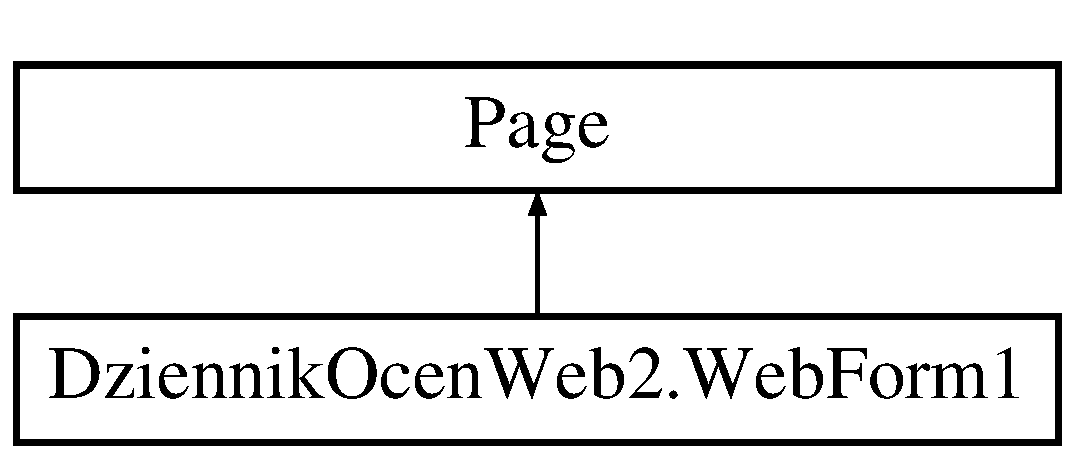
\includegraphics[height=2.000000cm]{class_dziennik_ocen_web2_1_1_web_form1}
\end{center}
\end{figure}
\subsection*{Public Member Functions}
\begin{DoxyCompactItemize}
\item 
\hyperlink{class_dziennik_ocen_web2_1_1_p_r_o_w_a_d_z_xC4_x84_c_y}{P\+R\+O\+W\+A\+D\+ZĄ\+CY} \hyperlink{class_dziennik_ocen_web2_1_1_web_form1_a2ba456de96b092f21e9a9a2d5a58f790}{Znajdz\+Prowadzacego} (string Email, string Haslo)
\item 
\hyperlink{class_dziennik_ocen_web2_1_1_s_t_u_d_e_n_t}{S\+T\+U\+D\+E\+NT} \hyperlink{class_dziennik_ocen_web2_1_1_web_form1_a2f9720fae025bfdbf899348616030c5c}{Znajdz\+Studenta} (string Email, string Haslo)
\item 
\hyperlink{class_dziennik_ocen_web2_1_1_p_r_o_j_e_k_t}{P\+R\+O\+J\+E\+KT} \hyperlink{class_dziennik_ocen_web2_1_1_web_form1_a5c395860f5810991b3791d6cfb099e67}{Znajdz\+Projekt} (int id)
\item 
\hyperlink{class_dziennik_ocen_web2_1_1_p_r_o_w_a_d_z_xC4_x84_c_y}{P\+R\+O\+W\+A\+D\+ZĄ\+CY} \hyperlink{class_dziennik_ocen_web2_1_1_web_form1_ade7bba3c68800a6cb44849abd379edc3}{Znajdz\+Prowadzacego} (int id\+\_\+przedmiotu)
\end{DoxyCompactItemize}
\subsection*{Protected Member Functions}
\begin{DoxyCompactItemize}
\item 
void \hyperlink{class_dziennik_ocen_web2_1_1_web_form1_ab279bd28af40dbba4b6c933af6666b27}{Page\+\_\+\+Load} (object sender, Event\+Args e)
\item 
void \hyperlink{class_dziennik_ocen_web2_1_1_web_form1_a51ab823b90323b205965fe55382e67e8}{Details\+View1\+\_\+\+Item\+Inserted} (object sender, Details\+View\+Inserted\+Event\+Args e)
\item 
void \hyperlink{class_dziennik_ocen_web2_1_1_web_form1_a231125238692401bbf89113d844e9e4b}{Button\+\_\+\+Dodaj\+Projekt\+\_\+\+Click} (object sender, Event\+Args e)
\item 
void \hyperlink{class_dziennik_ocen_web2_1_1_web_form1_a744c3c80bc4d8258797f13a886cd6087}{Button\+\_\+\+Dodaj\+Student\+\_\+\+Click} (object sender, Event\+Args e)
\item 
void \hyperlink{class_dziennik_ocen_web2_1_1_web_form1_aed94ee8575b41f7814a7955246d6ead4}{Button\+\_\+\+Dodaj\+Projekty\+\_\+\+Click} (object sender, Event\+Args e)
\item 
void \hyperlink{class_dziennik_ocen_web2_1_1_web_form1_a91c8516e0424804b520f798d112c6feb}{Button\+\_\+\+Dodaj\+Przedmioty\+\_\+\+Click} (object sender, Event\+Args e)
\item 
void \hyperlink{class_dziennik_ocen_web2_1_1_web_form1_a34bbbefe0677191a7a1927bbdfb52221}{Zaladuj\+Student} ()
\item 
void \hyperlink{class_dziennik_ocen_web2_1_1_web_form1_a1de7a96a7f82aeb38649a30c9fc9bb30}{Zaladuj\+Prowadzacy} ()
\item 
void \hyperlink{class_dziennik_ocen_web2_1_1_web_form1_a23f4a376efd1a0414fecdabc4457072b}{Zaladuj\+Admin} ()
\item 
void \hyperlink{class_dziennik_ocen_web2_1_1_web_form1_a42c9efde3f2521e876ec3e9ab6217b4f}{Button1\+\_\+\+Click} (object sender, Event\+Args e)
\item 
void \hyperlink{class_dziennik_ocen_web2_1_1_web_form1_aa743385735daea1ff89ee7942693aaec}{Button2\+\_\+\+Click} (object sender, Event\+Args e)
\item 
void \hyperlink{class_dziennik_ocen_web2_1_1_web_form1_aefb1ce8922cf82b4eb7e5e42e59b3f7d}{Button3\+\_\+\+Click} (object sender, Event\+Args e)
\item 
void \hyperlink{class_dziennik_ocen_web2_1_1_web_form1_a8b588699eca20966d75ba7e454ef01eb}{Button4\+\_\+\+Click} (object sender, Event\+Args e)
\item 
void \hyperlink{class_dziennik_ocen_web2_1_1_web_form1_a479205a9a82393a787866873176ab319}{Button\+\_\+\+Student\+\_\+zapiszsiedoprojektu\+\_\+\+Click} (object sender, Event\+Args e)
\end{DoxyCompactItemize}
\subsection*{Protected Attributes}
\begin{DoxyCompactItemize}
\item 
global\+::\+System.\+Web.\+U\+I.\+Html\+Controls.\+Html\+Form \hyperlink{class_dziennik_ocen_web2_1_1_web_form1_a38e3f99a2267a717e7772882a702c62c}{form1}
\begin{DoxyCompactList}\small\item\em form1 control. \end{DoxyCompactList}\item 
global\+::\+System.\+Web.\+U\+I.\+Web\+Controls.\+Text\+Box \hyperlink{class_dziennik_ocen_web2_1_1_web_form1_afd5c6cbba56f97163e3a77eacbe9f0c5}{Text\+Box\+Email}
\begin{DoxyCompactList}\small\item\em Text\+Box\+Email control. \end{DoxyCompactList}\item 
global\+::\+System.\+Web.\+U\+I.\+Web\+Controls.\+Text\+Box \hyperlink{class_dziennik_ocen_web2_1_1_web_form1_a243a5ae21436ccb946bb3e2e9bc4ae42}{Text\+Box\+Haslo}
\begin{DoxyCompactList}\small\item\em Text\+Box\+Haslo control. \end{DoxyCompactList}\item 
global\+::\+System.\+Web.\+U\+I.\+Web\+Controls.\+Button \hyperlink{class_dziennik_ocen_web2_1_1_web_form1_a14acc2b65cea9aecb77bb7d56ba12af6}{Button1}
\begin{DoxyCompactList}\small\item\em Button1 control. \end{DoxyCompactList}\item 
global\+::\+System.\+Web.\+U\+I.\+Web\+Controls.\+Button \hyperlink{class_dziennik_ocen_web2_1_1_web_form1_ae9c1f486a6ca18c24b98d8068c6a1414}{Button2}
\begin{DoxyCompactList}\small\item\em Button2 control. \end{DoxyCompactList}\item 
global\+::\+System.\+Web.\+U\+I.\+Web\+Controls.\+Button \hyperlink{class_dziennik_ocen_web2_1_1_web_form1_ad982d188e8e6201092bbafd8b038e81b}{Button3}
\begin{DoxyCompactList}\small\item\em Button3 control. \end{DoxyCompactList}\item 
global\+::\+System.\+Web.\+U\+I.\+Web\+Controls.\+Button \hyperlink{class_dziennik_ocen_web2_1_1_web_form1_aa4803d21f02860b91efc5823048e7ac4}{Button4}
\begin{DoxyCompactList}\small\item\em Button4 control. \end{DoxyCompactList}\item 
global\+::\+System.\+Web.\+U\+I.\+Html\+Controls.\+Html\+Table\+Row \hyperlink{class_dziennik_ocen_web2_1_1_web_form1_a5706de5be7075aed0566131920df6527}{Przedmiott}
\begin{DoxyCompactList}\small\item\em Przedmiott control. \end{DoxyCompactList}\item 
global\+::\+System.\+Web.\+U\+I.\+Web\+Controls.\+Grid\+View \hyperlink{class_dziennik_ocen_web2_1_1_web_form1_a33d6314fc2cc5c707fbc53f0ce93908e}{gv\+Przedmiot}
\begin{DoxyCompactList}\small\item\em gv\+Przedmiot control. \end{DoxyCompactList}\item 
global\+::\+System.\+Web.\+U\+I.\+Web\+Controls.\+Details\+View \hyperlink{class_dziennik_ocen_web2_1_1_web_form1_a1bae21a51b6446e066217e8a254a9cfc}{Details\+View1}
\begin{DoxyCompactList}\small\item\em Details\+View1 control. \end{DoxyCompactList}\item 
global\+::\+System.\+Web.\+U\+I.\+Html\+Controls.\+Html\+Table\+Row \hyperlink{class_dziennik_ocen_web2_1_1_web_form1_a6cf49628fc56b7e4e4078b13eef62dfd}{Projektt}
\begin{DoxyCompactList}\small\item\em Projektt control. \end{DoxyCompactList}\item 
global\+::\+System.\+Web.\+U\+I.\+Web\+Controls.\+Grid\+View \hyperlink{class_dziennik_ocen_web2_1_1_web_form1_ad32551b9a63fc02d922b608812673ccb}{gv\+Projekt}
\begin{DoxyCompactList}\small\item\em gv\+Projekt control. \end{DoxyCompactList}\item 
global\+::\+System.\+Web.\+U\+I.\+Html\+Controls.\+Html\+Table \hyperlink{class_dziennik_ocen_web2_1_1_web_form1_a3d1e1b225ea5a19d3331647f8f3a76ca}{Projekt\+Table}
\begin{DoxyCompactList}\small\item\em Projekt\+Table control. \end{DoxyCompactList}\item 
global\+::\+System.\+Web.\+U\+I.\+Html\+Controls.\+Html\+Table\+Row \hyperlink{class_dziennik_ocen_web2_1_1_web_form1_a9f87493b2d238e2f692040b0a55a87cc}{Projekt\+ID}
\begin{DoxyCompactList}\small\item\em Projekt\+ID control. \end{DoxyCompactList}\item 
global\+::\+System.\+Web.\+U\+I.\+Web\+Controls.\+Drop\+Down\+List \hyperlink{class_dziennik_ocen_web2_1_1_web_form1_aa1dcca0113aa3e8d239ef6fe3c91dadd}{Drop\+Down\+List\+\_\+\+Projekt\+\_\+id\+Przedmiotu}
\begin{DoxyCompactList}\small\item\em Drop\+Down\+List\+\_\+\+Projekt\+\_\+id\+Przedmiotu control. \end{DoxyCompactList}\item 
global\+::\+System.\+Web.\+U\+I.\+Html\+Controls.\+Html\+Table\+Row \hyperlink{class_dziennik_ocen_web2_1_1_web_form1_ad9257899086740c1e15537b8771eb526}{Projekt\+Nazwa}
\begin{DoxyCompactList}\small\item\em Projekt\+Nazwa control. \end{DoxyCompactList}\item 
global\+::\+System.\+Web.\+U\+I.\+Web\+Controls.\+Text\+Box \hyperlink{class_dziennik_ocen_web2_1_1_web_form1_a9ffad4170ae3c4a41c89ea8ff21f5c79}{Text\+Box\+\_\+\+Projekt\+\_\+nazwa\+Projektu}
\begin{DoxyCompactList}\small\item\em Text\+Box\+\_\+\+Projekt\+\_\+nazwa\+Projektu control. \end{DoxyCompactList}\item 
global\+::\+System.\+Web.\+U\+I.\+Html\+Controls.\+Html\+Table\+Row \hyperlink{class_dziennik_ocen_web2_1_1_web_form1_a3e54e8806cd16e24a83f6116805b5db1}{Projekt\+Opis}
\begin{DoxyCompactList}\small\item\em Projekt\+Opis control. \end{DoxyCompactList}\item 
global\+::\+System.\+Web.\+U\+I.\+Web\+Controls.\+Text\+Box \hyperlink{class_dziennik_ocen_web2_1_1_web_form1_a6ea6a10c6b9029ab3963c4032019257f}{Text\+Box\+\_\+\+Projekt\+\_\+opis\+Projektu}
\begin{DoxyCompactList}\small\item\em Text\+Box\+\_\+\+Projekt\+\_\+opis\+Projektu control. \end{DoxyCompactList}\item 
global\+::\+System.\+Web.\+U\+I.\+Web\+Controls.\+Button \hyperlink{class_dziennik_ocen_web2_1_1_web_form1_a9fce9205408b95c8ca305b3c235032d1}{Button\+\_\+\+Dodaj\+Projekt}
\begin{DoxyCompactList}\small\item\em Button\+\_\+\+Dodaj\+Projekt control. \end{DoxyCompactList}\item 
global\+::\+System.\+Web.\+U\+I.\+Web\+Controls.\+Drop\+Down\+List \hyperlink{class_dziennik_ocen_web2_1_1_web_form1_a4f4cb6542c912f6973422fe6db30d233}{Drop\+Down\+List\+\_\+\+Student\+\_\+zapiszsiedoprojektu}
\begin{DoxyCompactList}\small\item\em Drop\+Down\+List\+\_\+\+Student\+\_\+zapiszsiedoprojektu control. \end{DoxyCompactList}\item 
global\+::\+System.\+Web.\+U\+I.\+Web\+Controls.\+Button \hyperlink{class_dziennik_ocen_web2_1_1_web_form1_aa90a53487f082ae6c9124c782abd0678}{Button\+\_\+\+Student\+\_\+zapiszsiedoprojektu}
\begin{DoxyCompactList}\small\item\em Button\+\_\+\+Student\+\_\+zapiszsiedoprojektu control. \end{DoxyCompactList}\item 
global\+::\+System.\+Web.\+U\+I.\+Html\+Controls.\+Html\+Table\+Row \hyperlink{class_dziennik_ocen_web2_1_1_web_form1_a60e5d184ead042ff03cec6a6f956f9ba}{Grupaa}
\begin{DoxyCompactList}\small\item\em Grupaa control. \end{DoxyCompactList}\item 
global\+::\+System.\+Web.\+U\+I.\+Web\+Controls.\+Grid\+View \hyperlink{class_dziennik_ocen_web2_1_1_web_form1_a0c2630436cb78a1aa9de889b4961ea4f}{gv\+Grupa}
\begin{DoxyCompactList}\small\item\em gv\+Grupa control. \end{DoxyCompactList}\item 
global\+::\+System.\+Web.\+U\+I.\+Web\+Controls.\+Details\+View \hyperlink{class_dziennik_ocen_web2_1_1_web_form1_ac5d39d20de2956bae8ae9c23e148375f}{Details\+View2}
\begin{DoxyCompactList}\small\item\em Details\+View2 control. \end{DoxyCompactList}\item 
global\+::\+System.\+Web.\+U\+I.\+Html\+Controls.\+Html\+Table\+Row \hyperlink{class_dziennik_ocen_web2_1_1_web_form1_aea29c07bdcfe5faa4ec1cccba2cefdbc}{Studentt}
\begin{DoxyCompactList}\small\item\em Studentt control. \end{DoxyCompactList}\item 
global\+::\+System.\+Web.\+U\+I.\+Web\+Controls.\+Grid\+View \hyperlink{class_dziennik_ocen_web2_1_1_web_form1_a6d19631d031ec79157e86874ba97ba53}{gv\+Student}
\begin{DoxyCompactList}\small\item\em gv\+Student control. \end{DoxyCompactList}\item 
global\+::\+System.\+Web.\+U\+I.\+Web\+Controls.\+Drop\+Down\+List \hyperlink{class_dziennik_ocen_web2_1_1_web_form1_aadc0ea85a73c5483e41f6530a6bd63e5}{Drop\+Down\+List\+\_\+\+Student\+\_\+id\+Grupy}
\begin{DoxyCompactList}\small\item\em Drop\+Down\+List\+\_\+\+Student\+\_\+id\+Grupy control. \end{DoxyCompactList}\item 
global\+::\+System.\+Web.\+U\+I.\+Web\+Controls.\+Text\+Box \hyperlink{class_dziennik_ocen_web2_1_1_web_form1_a239f7a307a6f095d48231922986bb266}{Text\+Box\+\_\+\+Student\+\_\+imie}
\begin{DoxyCompactList}\small\item\em Text\+Box\+\_\+\+Student\+\_\+imie control. \end{DoxyCompactList}\item 
global\+::\+System.\+Web.\+U\+I.\+Web\+Controls.\+Text\+Box \hyperlink{class_dziennik_ocen_web2_1_1_web_form1_a161c5620ac7416db86706166470fd9f4}{Text\+Box\+\_\+\+Student\+\_\+nazwisko}
\begin{DoxyCompactList}\small\item\em Text\+Box\+\_\+\+Student\+\_\+nazwisko control. \end{DoxyCompactList}\item 
global\+::\+System.\+Web.\+U\+I.\+Web\+Controls.\+Text\+Box \hyperlink{class_dziennik_ocen_web2_1_1_web_form1_a21c07d34e93b30186e57f2a7e6786389}{Text\+Box\+\_\+\+Student\+\_\+telefon}
\begin{DoxyCompactList}\small\item\em Text\+Box\+\_\+\+Student\+\_\+telefon control. \end{DoxyCompactList}\item 
global\+::\+System.\+Web.\+U\+I.\+Web\+Controls.\+Text\+Box \hyperlink{class_dziennik_ocen_web2_1_1_web_form1_a36396ec2cf6138ceca37d487ee5b3bd0}{Text\+Box\+\_\+\+Student\+\_\+adres}
\begin{DoxyCompactList}\small\item\em Text\+Box\+\_\+\+Student\+\_\+adres control. \end{DoxyCompactList}\item 
global\+::\+System.\+Web.\+U\+I.\+Web\+Controls.\+Text\+Box \hyperlink{class_dziennik_ocen_web2_1_1_web_form1_afee4730e92c30198c0ed19d8fcfbe9a7}{Text\+Box\+\_\+\+Student\+\_\+email}
\begin{DoxyCompactList}\small\item\em Text\+Box\+\_\+\+Student\+\_\+email control. \end{DoxyCompactList}\item 
global\+::\+System.\+Web.\+U\+I.\+Web\+Controls.\+Text\+Box \hyperlink{class_dziennik_ocen_web2_1_1_web_form1_a0585ebb82159573ec49d9f45cb41e867}{Text\+Box\+\_\+\+Student\+\_\+haslo}
\begin{DoxyCompactList}\small\item\em Text\+Box\+\_\+\+Student\+\_\+haslo control. \end{DoxyCompactList}\item 
global\+::\+System.\+Web.\+U\+I.\+Web\+Controls.\+Button \hyperlink{class_dziennik_ocen_web2_1_1_web_form1_a4edf892602856b446ff7faa57b3cd60d}{Button\+\_\+\+Dodaj\+Student}
\begin{DoxyCompactList}\small\item\em Button\+\_\+\+Dodaj\+Student control. \end{DoxyCompactList}\item 
global\+::\+System.\+Web.\+U\+I.\+Html\+Controls.\+Html\+Table\+Row \hyperlink{class_dziennik_ocen_web2_1_1_web_form1_a09925c3ffc18a518cf5b176db72f0d6a}{Prowadzacyy}
\begin{DoxyCompactList}\small\item\em Prowadzacyy control. \end{DoxyCompactList}\item 
global\+::\+System.\+Web.\+U\+I.\+Web\+Controls.\+Grid\+View \hyperlink{class_dziennik_ocen_web2_1_1_web_form1_a9ee1e1f33472450888de9bbc4834a8bf}{gv\+Prowadzacy}
\begin{DoxyCompactList}\small\item\em gv\+Prowadzacy control. \end{DoxyCompactList}\item 
global\+::\+System.\+Web.\+U\+I.\+Web\+Controls.\+Details\+View \hyperlink{class_dziennik_ocen_web2_1_1_web_form1_a443cb784237ae454b881943bac17f87c}{Details\+View3}
\begin{DoxyCompactList}\small\item\em Details\+View3 control. \end{DoxyCompactList}\item 
global\+::\+System.\+Web.\+U\+I.\+Html\+Controls.\+Html\+Table\+Row \hyperlink{class_dziennik_ocen_web2_1_1_web_form1_abf93e1b3c58fc95ac0713ccadd807ef5}{Projektyy}
\begin{DoxyCompactList}\small\item\em Projektyy control. \end{DoxyCompactList}\item 
global\+::\+System.\+Web.\+U\+I.\+Web\+Controls.\+Grid\+View \hyperlink{class_dziennik_ocen_web2_1_1_web_form1_a75d645f4e2a139ccb924f8f131652e6d}{gv\+Projekty}
\begin{DoxyCompactList}\small\item\em gv\+Projekty control. \end{DoxyCompactList}\item 
global\+::\+System.\+Web.\+U\+I.\+Html\+Controls.\+Html\+Table \hyperlink{class_dziennik_ocen_web2_1_1_web_form1_a99d8f4908b7fce78eec0a83fa6752ad3}{Projekty\+Table}
\begin{DoxyCompactList}\small\item\em Projekty\+Table control. \end{DoxyCompactList}\item 
global\+::\+System.\+Web.\+U\+I.\+Html\+Controls.\+Html\+Table\+Row \hyperlink{class_dziennik_ocen_web2_1_1_web_form1_a32a9ef95539a282ca16273742f9e5b7e}{Projekty\+I\+D\+Studenta}
\begin{DoxyCompactList}\small\item\em Projekty\+I\+D\+Studenta control. \end{DoxyCompactList}\item 
global\+::\+System.\+Web.\+U\+I.\+Web\+Controls.\+Drop\+Down\+List \hyperlink{class_dziennik_ocen_web2_1_1_web_form1_a69b23baf7f1d15ffcf03150e8fa133bd}{Drop\+Down\+List\+\_\+\+Projekty\+\_\+id\+Studenta}
\begin{DoxyCompactList}\small\item\em Drop\+Down\+List\+\_\+\+Projekty\+\_\+id\+Studenta control. \end{DoxyCompactList}\item 
global\+::\+System.\+Web.\+U\+I.\+Html\+Controls.\+Html\+Table\+Row \hyperlink{class_dziennik_ocen_web2_1_1_web_form1_a2d974557e638f29db410389b93af4cf3}{Projekty\+I\+D\+Projektu}
\begin{DoxyCompactList}\small\item\em Projekty\+I\+D\+Projektu control. \end{DoxyCompactList}\item 
global\+::\+System.\+Web.\+U\+I.\+Web\+Controls.\+Drop\+Down\+List \hyperlink{class_dziennik_ocen_web2_1_1_web_form1_a5a3d84b013408bc386a35d766eb2afdf}{Drop\+Down\+List\+\_\+\+Projekty\+\_\+id\+Projektu}
\begin{DoxyCompactList}\small\item\em Drop\+Down\+List\+\_\+\+Projekty\+\_\+id\+Projektu control. \end{DoxyCompactList}\item 
global\+::\+System.\+Web.\+U\+I.\+Html\+Controls.\+Html\+Table\+Row \hyperlink{class_dziennik_ocen_web2_1_1_web_form1_a7863d38f63d7d921beeadd58950adcbf}{Projekty\+I\+D\+Prowadzacego}
\begin{DoxyCompactList}\small\item\em Projekty\+I\+D\+Prowadzacego control. \end{DoxyCompactList}\item 
global\+::\+System.\+Web.\+U\+I.\+Web\+Controls.\+Drop\+Down\+List \hyperlink{class_dziennik_ocen_web2_1_1_web_form1_acd84cc06850f05e526a1aee42c1a72c5}{Drop\+Down\+List\+\_\+\+Projekty\+\_\+id\+Prowadzacego}
\begin{DoxyCompactList}\small\item\em Drop\+Down\+List\+\_\+\+Projekty\+\_\+id\+Prowadzacego control. \end{DoxyCompactList}\item 
global\+::\+System.\+Web.\+U\+I.\+Html\+Controls.\+Html\+Table\+Row \hyperlink{class_dziennik_ocen_web2_1_1_web_form1_ab0ee54e545af71912658fe0b23a3cdd9}{Projekty\+Ocena}
\begin{DoxyCompactList}\small\item\em Projekty\+Ocena control. \end{DoxyCompactList}\item 
global\+::\+System.\+Web.\+U\+I.\+Web\+Controls.\+Text\+Box \hyperlink{class_dziennik_ocen_web2_1_1_web_form1_aa4ba06f7e833012a4b33e57bc3850a5b}{Text\+Box\+\_\+\+Projekty\+\_\+ocena}
\begin{DoxyCompactList}\small\item\em Text\+Box\+\_\+\+Projekty\+\_\+ocena control. \end{DoxyCompactList}\item 
global\+::\+System.\+Web.\+U\+I.\+Html\+Controls.\+Html\+Table\+Row \hyperlink{class_dziennik_ocen_web2_1_1_web_form1_a9aa72d2cb06ee8300309d0965ec7cea2}{Projekty\+Data}
\begin{DoxyCompactList}\small\item\em Projekty\+Data control. \end{DoxyCompactList}\item 
global\+::\+System.\+Web.\+U\+I.\+Web\+Controls.\+Text\+Box \hyperlink{class_dziennik_ocen_web2_1_1_web_form1_a2f98d4ead21263b9c611a81eecbcbd24}{Text\+Box\+\_\+\+Projekty\+\_\+data\+Projektu}
\begin{DoxyCompactList}\small\item\em Text\+Box\+\_\+\+Projekty\+\_\+data\+Projektu control. \end{DoxyCompactList}\item 
global\+::\+System.\+Web.\+U\+I.\+Html\+Controls.\+Html\+Table\+Row \hyperlink{class_dziennik_ocen_web2_1_1_web_form1_a27e330c18393285c8f2e61279dee5106}{Projekty\+Uwagi}
\begin{DoxyCompactList}\small\item\em Projekty\+Uwagi control. \end{DoxyCompactList}\item 
global\+::\+System.\+Web.\+U\+I.\+Web\+Controls.\+Text\+Box \hyperlink{class_dziennik_ocen_web2_1_1_web_form1_a43df52d8c914980d8f9a8b377884aa09}{Text\+Box\+\_\+\+Projekty\+\_\+uwagi}
\begin{DoxyCompactList}\small\item\em Text\+Box\+\_\+\+Projekty\+\_\+uwagi control. \end{DoxyCompactList}\item 
global\+::\+System.\+Web.\+U\+I.\+Web\+Controls.\+Button \hyperlink{class_dziennik_ocen_web2_1_1_web_form1_a9ed89f06b0fd85c351236961f0a4a353}{Button\+\_\+\+Dodaj\+Projekty}
\begin{DoxyCompactList}\small\item\em Button\+\_\+\+Dodaj\+Projekty control. \end{DoxyCompactList}\item 
global\+::\+System.\+Web.\+U\+I.\+Html\+Controls.\+Html\+Table\+Row \hyperlink{class_dziennik_ocen_web2_1_1_web_form1_a61d033c16d4ca718f004f15f153463dd}{Przedmiotyy}
\begin{DoxyCompactList}\small\item\em Przedmiotyy control. \end{DoxyCompactList}\item 
global\+::\+System.\+Web.\+U\+I.\+Web\+Controls.\+Grid\+View \hyperlink{class_dziennik_ocen_web2_1_1_web_form1_ab823c042dbbcc237618e27b8734413cb}{gv\+Przedmioty}
\begin{DoxyCompactList}\small\item\em gv\+Przedmioty control. \end{DoxyCompactList}\item 
global\+::\+System.\+Web.\+U\+I.\+Html\+Controls.\+Html\+Table \hyperlink{class_dziennik_ocen_web2_1_1_web_form1_a1a76555165dbd95e98b2ca9324e5b4e7}{Przedmioty\+Table}
\begin{DoxyCompactList}\small\item\em Przedmioty\+Table control. \end{DoxyCompactList}\item 
global\+::\+System.\+Web.\+U\+I.\+Web\+Controls.\+Drop\+Down\+List \hyperlink{class_dziennik_ocen_web2_1_1_web_form1_aaf6a4d83bf0fcef855ca4a3efcf7461d}{Drop\+Down\+List\+\_\+\+Przedmioty\+\_\+id\+Studenta}
\begin{DoxyCompactList}\small\item\em Drop\+Down\+List\+\_\+\+Przedmioty\+\_\+id\+Studenta control. \end{DoxyCompactList}\item 
global\+::\+System.\+Web.\+U\+I.\+Web\+Controls.\+Drop\+Down\+List \hyperlink{class_dziennik_ocen_web2_1_1_web_form1_ac8114888f1541e455e45ae638204aefd}{Drop\+Down\+List\+\_\+\+Przedmioty\+\_\+id\+Prowadzacego}
\begin{DoxyCompactList}\small\item\em Drop\+Down\+List\+\_\+\+Przedmioty\+\_\+id\+Prowadzacego control. \end{DoxyCompactList}\item 
global\+::\+System.\+Web.\+U\+I.\+Web\+Controls.\+Drop\+Down\+List \hyperlink{class_dziennik_ocen_web2_1_1_web_form1_a94670ac4f330ade51b5796c88a5e7129}{Drop\+Down\+List\+\_\+\+Przedmioty\+\_\+id\+Przedmiotu}
\begin{DoxyCompactList}\small\item\em Drop\+Down\+List\+\_\+\+Przedmioty\+\_\+id\+Przedmiotu control. \end{DoxyCompactList}\item 
global\+::\+System.\+Web.\+U\+I.\+Html\+Controls.\+Html\+Table\+Row \hyperlink{class_dziennik_ocen_web2_1_1_web_form1_a5d9a4c5708b84c0eb5cb2de5b8eed5c9}{Przedmioty\+Ocena}
\begin{DoxyCompactList}\small\item\em Przedmioty\+Ocena control. \end{DoxyCompactList}\item 
global\+::\+System.\+Web.\+U\+I.\+Web\+Controls.\+Text\+Box \hyperlink{class_dziennik_ocen_web2_1_1_web_form1_acd1f8459612e926ade2856e75348ea7c}{Text\+Box\+\_\+\+Przedmioty\+\_\+ocena\+Przedmiotu}
\begin{DoxyCompactList}\small\item\em Text\+Box\+\_\+\+Przedmioty\+\_\+ocena\+Przedmiotu control. \end{DoxyCompactList}\item 
global\+::\+System.\+Web.\+U\+I.\+Html\+Controls.\+Html\+Table\+Row \hyperlink{class_dziennik_ocen_web2_1_1_web_form1_aaf454ed1f421284f7248d2428b442739}{Przedmioty\+Data}
\begin{DoxyCompactList}\small\item\em Przedmioty\+Data control. \end{DoxyCompactList}\item 
global\+::\+System.\+Web.\+U\+I.\+Web\+Controls.\+Text\+Box \hyperlink{class_dziennik_ocen_web2_1_1_web_form1_a53cf39cd0712712d4a869bd5c846aad7}{Text\+Box\+\_\+\+Przedmioty\+\_\+data\+Zaliczenia}
\begin{DoxyCompactList}\small\item\em Text\+Box\+\_\+\+Przedmioty\+\_\+data\+Zaliczenia control. \end{DoxyCompactList}\item 
global\+::\+System.\+Web.\+U\+I.\+Html\+Controls.\+Html\+Table\+Row \hyperlink{class_dziennik_ocen_web2_1_1_web_form1_af38d3b4fdef8737b1b414b0bf6ca6b60}{Przedmioty\+Uwagi}
\begin{DoxyCompactList}\small\item\em Przedmioty\+Uwagi control. \end{DoxyCompactList}\item 
global\+::\+System.\+Web.\+U\+I.\+Web\+Controls.\+Text\+Box \hyperlink{class_dziennik_ocen_web2_1_1_web_form1_ab9368c26118387c8cd81c23f679b2974}{Text\+Box\+\_\+\+Przedmioty\+\_\+uwagi}
\begin{DoxyCompactList}\small\item\em Text\+Box\+\_\+\+Przedmioty\+\_\+uwagi control. \end{DoxyCompactList}\item 
global\+::\+System.\+Web.\+U\+I.\+Web\+Controls.\+Button \hyperlink{class_dziennik_ocen_web2_1_1_web_form1_a71e8b22e9d07253f09658420f9cd762d}{Button\+\_\+\+Dodaj\+Przedmioty}
\begin{DoxyCompactList}\small\item\em Button\+\_\+\+Dodaj\+Przedmioty control. \end{DoxyCompactList}\item 
global\+::\+System.\+Web.\+U\+I.\+Html\+Controls.\+Html\+Table\+Row \hyperlink{class_dziennik_ocen_web2_1_1_web_form1_ab1eb7a8ef1345e0e57b0f969dfa07e85}{Przedmiotyy\+Konkretny}
\begin{DoxyCompactList}\small\item\em Przedmiotyy\+Konkretny control. \end{DoxyCompactList}\item 
global\+::\+System.\+Web.\+U\+I.\+Web\+Controls.\+Grid\+View \hyperlink{class_dziennik_ocen_web2_1_1_web_form1_abf211c7946ad1b40a27598c4ad2cbed2}{Grid\+View1}
\begin{DoxyCompactList}\small\item\em Grid\+View1 control. \end{DoxyCompactList}\item 
global\+::\+System.\+Web.\+U\+I.\+Html\+Controls.\+Html\+Table \hyperlink{class_dziennik_ocen_web2_1_1_web_form1_ae07ff54c565a4fd8deaa4b074af896cf}{Przedmioty\+Table0}
\begin{DoxyCompactList}\small\item\em Przedmioty\+Table0 control. \end{DoxyCompactList}\item 
global\+::\+System.\+Web.\+U\+I.\+Web\+Controls.\+Drop\+Down\+List \hyperlink{class_dziennik_ocen_web2_1_1_web_form1_aeb8404dae73cca5377a5bc6e86629837}{Drop\+Down\+List\+\_\+\+Przedmioty\+\_\+id\+Studenta0}
\begin{DoxyCompactList}\small\item\em Drop\+Down\+List\+\_\+\+Przedmioty\+\_\+id\+Studenta0 control. \end{DoxyCompactList}\item 
global\+::\+System.\+Web.\+U\+I.\+Web\+Controls.\+Drop\+Down\+List \hyperlink{class_dziennik_ocen_web2_1_1_web_form1_aa5510d7e77e936fa64b1f15ee29388ea}{Drop\+Down\+List\+\_\+\+Przedmioty\+\_\+id\+Prowadzacego0}
\begin{DoxyCompactList}\small\item\em Drop\+Down\+List\+\_\+\+Przedmioty\+\_\+id\+Prowadzacego0 control. \end{DoxyCompactList}\item 
global\+::\+System.\+Web.\+U\+I.\+Web\+Controls.\+Drop\+Down\+List \hyperlink{class_dziennik_ocen_web2_1_1_web_form1_a1db4ed91510910999787a86606986523}{Drop\+Down\+List\+\_\+\+Przedmioty\+\_\+id\+Przedmiotu0}
\begin{DoxyCompactList}\small\item\em Drop\+Down\+List\+\_\+\+Przedmioty\+\_\+id\+Przedmiotu0 control. \end{DoxyCompactList}\item 
global\+::\+System.\+Web.\+U\+I.\+Html\+Controls.\+Html\+Table\+Row \hyperlink{class_dziennik_ocen_web2_1_1_web_form1_a3060dcb1eb46e02e1f02ecfa2700129c}{Przedmioty\+Ocena0}
\begin{DoxyCompactList}\small\item\em Przedmioty\+Ocena0 control. \end{DoxyCompactList}\item 
global\+::\+System.\+Web.\+U\+I.\+Web\+Controls.\+Text\+Box \hyperlink{class_dziennik_ocen_web2_1_1_web_form1_a302ee9498b9e5c0bcf7fe1b8f81f3c5e}{Text\+Box\+\_\+\+Przedmioty\+\_\+ocena\+Przedmiotu0}
\begin{DoxyCompactList}\small\item\em Text\+Box\+\_\+\+Przedmioty\+\_\+ocena\+Przedmiotu0 control. \end{DoxyCompactList}\item 
global\+::\+System.\+Web.\+U\+I.\+Html\+Controls.\+Html\+Table\+Row \hyperlink{class_dziennik_ocen_web2_1_1_web_form1_a94d86e7b2aaea0179abc87aa43c3bbde}{Przedmioty\+Data0}
\begin{DoxyCompactList}\small\item\em Przedmioty\+Data0 control. \end{DoxyCompactList}\item 
global\+::\+System.\+Web.\+U\+I.\+Web\+Controls.\+Text\+Box \hyperlink{class_dziennik_ocen_web2_1_1_web_form1_ae72a9bfae3378226ad33914e0b3ae263}{Text\+Box\+\_\+\+Przedmioty\+\_\+data\+Zaliczenia0}
\begin{DoxyCompactList}\small\item\em Text\+Box\+\_\+\+Przedmioty\+\_\+data\+Zaliczenia0 control. \end{DoxyCompactList}\item 
global\+::\+System.\+Web.\+U\+I.\+Html\+Controls.\+Html\+Table\+Row \hyperlink{class_dziennik_ocen_web2_1_1_web_form1_ae0f27438f74a07309842a272e9010e1b}{Przedmioty\+Uwagi0}
\begin{DoxyCompactList}\small\item\em Przedmioty\+Uwagi0 control. \end{DoxyCompactList}\item 
global\+::\+System.\+Web.\+U\+I.\+Web\+Controls.\+Text\+Box \hyperlink{class_dziennik_ocen_web2_1_1_web_form1_adee12d3b9fb7aed5f516c70ce4d5a114}{Text\+Box\+\_\+\+Przedmioty\+\_\+uwagi0}
\begin{DoxyCompactList}\small\item\em Text\+Box\+\_\+\+Przedmioty\+\_\+uwagi0 control. \end{DoxyCompactList}\item 
global\+::\+System.\+Web.\+U\+I.\+Web\+Controls.\+Button \hyperlink{class_dziennik_ocen_web2_1_1_web_form1_a8c864c9ae0eb563508b3b1a87612b8f0}{Button\+\_\+\+Dodaj\+Przedmioty0}
\begin{DoxyCompactList}\small\item\em Button\+\_\+\+Dodaj\+Przedmioty0 control. \end{DoxyCompactList}\item 
global\+::\+System.\+Web.\+U\+I.\+Html\+Controls.\+Html\+Table\+Row \hyperlink{class_dziennik_ocen_web2_1_1_web_form1_a236a0340a0cdd4be0cb04f8231c70c79}{Projektyy\+Konkretny}
\begin{DoxyCompactList}\small\item\em Projektyy\+Konkretny control. \end{DoxyCompactList}\item 
global\+::\+System.\+Web.\+U\+I.\+Web\+Controls.\+Grid\+View \hyperlink{class_dziennik_ocen_web2_1_1_web_form1_a835a3a863f668e7f4d1b9f8d1e82a933}{Grid\+View2}
\begin{DoxyCompactList}\small\item\em Grid\+View2 control. \end{DoxyCompactList}\item 
global\+::\+System.\+Web.\+U\+I.\+Html\+Controls.\+Html\+Table \hyperlink{class_dziennik_ocen_web2_1_1_web_form1_a218e50105cfbf5e9c4c218f1098e2e00}{Projekty\+Table0}
\begin{DoxyCompactList}\small\item\em Projekty\+Table0 control. \end{DoxyCompactList}\item 
global\+::\+System.\+Web.\+U\+I.\+Html\+Controls.\+Html\+Table\+Row \hyperlink{class_dziennik_ocen_web2_1_1_web_form1_a1a4e38055cff20b9c979b9a72608f5d7}{Projekty\+I\+D\+Studenta0}
\begin{DoxyCompactList}\small\item\em Projekty\+I\+D\+Studenta0 control. \end{DoxyCompactList}\item 
global\+::\+System.\+Web.\+U\+I.\+Web\+Controls.\+Drop\+Down\+List \hyperlink{class_dziennik_ocen_web2_1_1_web_form1_a56263d1234f7811a3793deae16255be1}{Drop\+Down\+List\+\_\+\+Projekty\+\_\+id\+Studenta0}
\begin{DoxyCompactList}\small\item\em Drop\+Down\+List\+\_\+\+Projekty\+\_\+id\+Studenta0 control. \end{DoxyCompactList}\item 
global\+::\+System.\+Web.\+U\+I.\+Html\+Controls.\+Html\+Table\+Row \hyperlink{class_dziennik_ocen_web2_1_1_web_form1_a2c3f09e98eb048a17c692bf0589e5035}{Projekty\+I\+D\+Projektu0}
\begin{DoxyCompactList}\small\item\em Projekty\+I\+D\+Projektu0 control. \end{DoxyCompactList}\item 
global\+::\+System.\+Web.\+U\+I.\+Web\+Controls.\+Drop\+Down\+List \hyperlink{class_dziennik_ocen_web2_1_1_web_form1_a533bb90bea691dda0884d9d977e0af55}{Drop\+Down\+List\+\_\+\+Projekty\+\_\+id\+Projektu0}
\begin{DoxyCompactList}\small\item\em Drop\+Down\+List\+\_\+\+Projekty\+\_\+id\+Projektu0 control. \end{DoxyCompactList}\item 
global\+::\+System.\+Web.\+U\+I.\+Html\+Controls.\+Html\+Table\+Row \hyperlink{class_dziennik_ocen_web2_1_1_web_form1_a2cf2d616a26c3cc1b02d3e0b8aa47690}{Projekty\+I\+D\+Prowadzacego0}
\begin{DoxyCompactList}\small\item\em Projekty\+I\+D\+Prowadzacego0 control. \end{DoxyCompactList}\item 
global\+::\+System.\+Web.\+U\+I.\+Web\+Controls.\+Drop\+Down\+List \hyperlink{class_dziennik_ocen_web2_1_1_web_form1_a48e6225cc66d43f62efa99625485d3db}{Drop\+Down\+List\+\_\+\+Projekty\+\_\+id\+Prowadzacego0}
\begin{DoxyCompactList}\small\item\em Drop\+Down\+List\+\_\+\+Projekty\+\_\+id\+Prowadzacego0 control. \end{DoxyCompactList}\item 
global\+::\+System.\+Web.\+U\+I.\+Html\+Controls.\+Html\+Table\+Row \hyperlink{class_dziennik_ocen_web2_1_1_web_form1_a55cb47e538e27de5daac8a1f325eed64}{Projekty\+Ocena0}
\begin{DoxyCompactList}\small\item\em Projekty\+Ocena0 control. \end{DoxyCompactList}\item 
global\+::\+System.\+Web.\+U\+I.\+Web\+Controls.\+Text\+Box \hyperlink{class_dziennik_ocen_web2_1_1_web_form1_a5a77cbbbe25b39b4f8a5639be94ac841}{Text\+Box\+\_\+\+Projekty\+\_\+ocena0}
\begin{DoxyCompactList}\small\item\em Text\+Box\+\_\+\+Projekty\+\_\+ocena0 control. \end{DoxyCompactList}\item 
global\+::\+System.\+Web.\+U\+I.\+Html\+Controls.\+Html\+Table\+Row \hyperlink{class_dziennik_ocen_web2_1_1_web_form1_a041f44ddf339d8b10a89bfcad55a58a7}{Projekty\+Data0}
\begin{DoxyCompactList}\small\item\em Projekty\+Data0 control. \end{DoxyCompactList}\item 
global\+::\+System.\+Web.\+U\+I.\+Web\+Controls.\+Text\+Box \hyperlink{class_dziennik_ocen_web2_1_1_web_form1_aebb640122d0045069b76a51dd72d86be}{Text\+Box\+\_\+\+Projekty\+\_\+data\+Projektu0}
\begin{DoxyCompactList}\small\item\em Text\+Box\+\_\+\+Projekty\+\_\+data\+Projektu0 control. \end{DoxyCompactList}\item 
global\+::\+System.\+Web.\+U\+I.\+Html\+Controls.\+Html\+Table\+Row \hyperlink{class_dziennik_ocen_web2_1_1_web_form1_a7242c14fa14fc26f3f1413d95e986d4f}{Projekty\+Uwagi0}
\begin{DoxyCompactList}\small\item\em Projekty\+Uwagi0 control. \end{DoxyCompactList}\item 
global\+::\+System.\+Web.\+U\+I.\+Web\+Controls.\+Text\+Box \hyperlink{class_dziennik_ocen_web2_1_1_web_form1_a8816d59dd0d3387f0bc5f4b22df7e73d}{Text\+Box\+\_\+\+Projekty\+\_\+uwagi0}
\begin{DoxyCompactList}\small\item\em Text\+Box\+\_\+\+Projekty\+\_\+uwagi0 control. \end{DoxyCompactList}\item 
global\+::\+System.\+Web.\+U\+I.\+Web\+Controls.\+Button \hyperlink{class_dziennik_ocen_web2_1_1_web_form1_a116551ad032492cd511786a64b19b21c}{Button\+\_\+\+Dodaj\+Projekty0}
\begin{DoxyCompactList}\small\item\em Button\+\_\+\+Dodaj\+Projekty0 control. \end{DoxyCompactList}\item 
global\+::\+System.\+Web.\+U\+I.\+Web\+Controls.\+Entity\+Data\+Source \hyperlink{class_dziennik_ocen_web2_1_1_web_form1_a24319b93de14462cd162625f5e6fc97e}{eds\+Przedmiot}
\begin{DoxyCompactList}\small\item\em eds\+Przedmiot control. \end{DoxyCompactList}\item 
global\+::\+System.\+Web.\+U\+I.\+Web\+Controls.\+Entity\+Data\+Source \hyperlink{class_dziennik_ocen_web2_1_1_web_form1_a6e12616cfa2c7a68fae19a52ae8ff00d}{eds\+Projekt}
\begin{DoxyCompactList}\small\item\em eds\+Projekt control. \end{DoxyCompactList}\item 
global\+::\+System.\+Web.\+U\+I.\+Web\+Controls.\+Entity\+Data\+Source \hyperlink{class_dziennik_ocen_web2_1_1_web_form1_aff2babfe7a3e4024805e43082cb63817}{eds\+Grupa}
\begin{DoxyCompactList}\small\item\em eds\+Grupa control. \end{DoxyCompactList}\item 
global\+::\+System.\+Web.\+U\+I.\+Web\+Controls.\+Entity\+Data\+Source \hyperlink{class_dziennik_ocen_web2_1_1_web_form1_a24e676704e911424646f8dcf6da4168a}{eds\+Student}
\begin{DoxyCompactList}\small\item\em eds\+Student control. \end{DoxyCompactList}\item 
global\+::\+System.\+Web.\+U\+I.\+Web\+Controls.\+Entity\+Data\+Source \hyperlink{class_dziennik_ocen_web2_1_1_web_form1_a7e32f1f4686ffa1bbafd6ddbd4cfade3}{eds\+Prowadzacy}
\begin{DoxyCompactList}\small\item\em eds\+Prowadzacy control. \end{DoxyCompactList}\item 
global\+::\+System.\+Web.\+U\+I.\+Web\+Controls.\+Entity\+Data\+Source \hyperlink{class_dziennik_ocen_web2_1_1_web_form1_a32e1d11a35d684b6ab04cae7227c87f9}{eds\+Projekty}
\begin{DoxyCompactList}\small\item\em eds\+Projekty control. \end{DoxyCompactList}\item 
global\+::\+System.\+Web.\+U\+I.\+Web\+Controls.\+Entity\+Data\+Source \hyperlink{class_dziennik_ocen_web2_1_1_web_form1_ada8b054b3125429b79a37e9b7fd56e0b}{eds\+Przedmioty}
\begin{DoxyCompactList}\small\item\em eds\+Przedmioty control. \end{DoxyCompactList}\item 
global\+::\+System.\+Web.\+U\+I.\+Web\+Controls.\+Entity\+Data\+Source \hyperlink{class_dziennik_ocen_web2_1_1_web_form1_a33092eb5bfd56d84a256312d7c6e1b49}{eds\+Przedmioty\+Konkretny}
\begin{DoxyCompactList}\small\item\em eds\+Przedmioty\+Konkretny control. \end{DoxyCompactList}\item 
global\+::\+System.\+Web.\+U\+I.\+Web\+Controls.\+Entity\+Data\+Source \hyperlink{class_dziennik_ocen_web2_1_1_web_form1_a6a1fedb3c8893198f5063d95b0996840}{eds\+Projekty\+Konkretny}
\begin{DoxyCompactList}\small\item\em eds\+Projekty\+Konkretny control. \end{DoxyCompactList}\end{DoxyCompactItemize}
\subsection*{Private Attributes}
\begin{DoxyCompactItemize}
\item 
\hyperlink{class_dziennik_ocen_web2_1_1_dziennik_ocen_entities}{Dziennik\+Ocen\+Entities} \hyperlink{class_dziennik_ocen_web2_1_1_web_form1_a8247555bffb3698fe1d03a15b2253840}{db} = new \hyperlink{class_dziennik_ocen_web2_1_1_dziennik_ocen_entities}{Dziennik\+Ocen\+Entities}()
\item 
\hyperlink{class_dziennik_ocen_web2_1_1projekty}{projekty} \hyperlink{class_dziennik_ocen_web2_1_1_web_form1_a74f7f160ce70c171580e9b402519ef0c}{projekty}
\item 
\hyperlink{class_dziennik_ocen_web2_1_1_p_r_o_j_e_k_t}{P\+R\+O\+J\+E\+KT} \hyperlink{class_dziennik_ocen_web2_1_1_web_form1_a562d751bd052452a169239c1445f196c}{projekt}
\item 
\hyperlink{class_dziennik_ocen_web2_1_1_p_r_o_w_a_d_z_xC4_x84_c_y}{P\+R\+O\+W\+A\+D\+ZĄ\+CY} \hyperlink{class_dziennik_ocen_web2_1_1_web_form1_a85d951a7def4f525c11c98d11725712d}{prowadzacy}
\item 
\hyperlink{class_dziennik_ocen_web2_1_1_s_t_u_d_e_n_t}{S\+T\+U\+D\+E\+NT} \hyperlink{class_dziennik_ocen_web2_1_1_web_form1_a91ac405a6d3e3a700685501c6ea67fb0}{student}
\end{DoxyCompactItemize}


\subsection{Member Function Documentation}
\mbox{\Hypertarget{class_dziennik_ocen_web2_1_1_web_form1_a42c9efde3f2521e876ec3e9ab6217b4f}\label{class_dziennik_ocen_web2_1_1_web_form1_a42c9efde3f2521e876ec3e9ab6217b4f}} 
\index{Dziennik\+Ocen\+Web2\+::\+Web\+Form1@{Dziennik\+Ocen\+Web2\+::\+Web\+Form1}!Button1\+\_\+\+Click@{Button1\+\_\+\+Click}}
\index{Button1\+\_\+\+Click@{Button1\+\_\+\+Click}!Dziennik\+Ocen\+Web2\+::\+Web\+Form1@{Dziennik\+Ocen\+Web2\+::\+Web\+Form1}}
\subsubsection{\texorpdfstring{Button1\+\_\+\+Click()}{Button1\_Click()}}
{\footnotesize\ttfamily void Dziennik\+Ocen\+Web2.\+Web\+Form1.\+Button1\+\_\+\+Click (\begin{DoxyParamCaption}\item[{object}]{sender,  }\item[{Event\+Args}]{e }\end{DoxyParamCaption})\hspace{0.3cm}{\ttfamily [inline]}, {\ttfamily [protected]}}

\mbox{\Hypertarget{class_dziennik_ocen_web2_1_1_web_form1_aa743385735daea1ff89ee7942693aaec}\label{class_dziennik_ocen_web2_1_1_web_form1_aa743385735daea1ff89ee7942693aaec}} 
\index{Dziennik\+Ocen\+Web2\+::\+Web\+Form1@{Dziennik\+Ocen\+Web2\+::\+Web\+Form1}!Button2\+\_\+\+Click@{Button2\+\_\+\+Click}}
\index{Button2\+\_\+\+Click@{Button2\+\_\+\+Click}!Dziennik\+Ocen\+Web2\+::\+Web\+Form1@{Dziennik\+Ocen\+Web2\+::\+Web\+Form1}}
\subsubsection{\texorpdfstring{Button2\+\_\+\+Click()}{Button2\_Click()}}
{\footnotesize\ttfamily void Dziennik\+Ocen\+Web2.\+Web\+Form1.\+Button2\+\_\+\+Click (\begin{DoxyParamCaption}\item[{object}]{sender,  }\item[{Event\+Args}]{e }\end{DoxyParamCaption})\hspace{0.3cm}{\ttfamily [inline]}, {\ttfamily [protected]}}

\mbox{\Hypertarget{class_dziennik_ocen_web2_1_1_web_form1_aefb1ce8922cf82b4eb7e5e42e59b3f7d}\label{class_dziennik_ocen_web2_1_1_web_form1_aefb1ce8922cf82b4eb7e5e42e59b3f7d}} 
\index{Dziennik\+Ocen\+Web2\+::\+Web\+Form1@{Dziennik\+Ocen\+Web2\+::\+Web\+Form1}!Button3\+\_\+\+Click@{Button3\+\_\+\+Click}}
\index{Button3\+\_\+\+Click@{Button3\+\_\+\+Click}!Dziennik\+Ocen\+Web2\+::\+Web\+Form1@{Dziennik\+Ocen\+Web2\+::\+Web\+Form1}}
\subsubsection{\texorpdfstring{Button3\+\_\+\+Click()}{Button3\_Click()}}
{\footnotesize\ttfamily void Dziennik\+Ocen\+Web2.\+Web\+Form1.\+Button3\+\_\+\+Click (\begin{DoxyParamCaption}\item[{object}]{sender,  }\item[{Event\+Args}]{e }\end{DoxyParamCaption})\hspace{0.3cm}{\ttfamily [inline]}, {\ttfamily [protected]}}

\mbox{\Hypertarget{class_dziennik_ocen_web2_1_1_web_form1_a8b588699eca20966d75ba7e454ef01eb}\label{class_dziennik_ocen_web2_1_1_web_form1_a8b588699eca20966d75ba7e454ef01eb}} 
\index{Dziennik\+Ocen\+Web2\+::\+Web\+Form1@{Dziennik\+Ocen\+Web2\+::\+Web\+Form1}!Button4\+\_\+\+Click@{Button4\+\_\+\+Click}}
\index{Button4\+\_\+\+Click@{Button4\+\_\+\+Click}!Dziennik\+Ocen\+Web2\+::\+Web\+Form1@{Dziennik\+Ocen\+Web2\+::\+Web\+Form1}}
\subsubsection{\texorpdfstring{Button4\+\_\+\+Click()}{Button4\_Click()}}
{\footnotesize\ttfamily void Dziennik\+Ocen\+Web2.\+Web\+Form1.\+Button4\+\_\+\+Click (\begin{DoxyParamCaption}\item[{object}]{sender,  }\item[{Event\+Args}]{e }\end{DoxyParamCaption})\hspace{0.3cm}{\ttfamily [inline]}, {\ttfamily [protected]}}

\mbox{\Hypertarget{class_dziennik_ocen_web2_1_1_web_form1_a231125238692401bbf89113d844e9e4b}\label{class_dziennik_ocen_web2_1_1_web_form1_a231125238692401bbf89113d844e9e4b}} 
\index{Dziennik\+Ocen\+Web2\+::\+Web\+Form1@{Dziennik\+Ocen\+Web2\+::\+Web\+Form1}!Button\+\_\+\+Dodaj\+Projekt\+\_\+\+Click@{Button\+\_\+\+Dodaj\+Projekt\+\_\+\+Click}}
\index{Button\+\_\+\+Dodaj\+Projekt\+\_\+\+Click@{Button\+\_\+\+Dodaj\+Projekt\+\_\+\+Click}!Dziennik\+Ocen\+Web2\+::\+Web\+Form1@{Dziennik\+Ocen\+Web2\+::\+Web\+Form1}}
\subsubsection{\texorpdfstring{Button\+\_\+\+Dodaj\+Projekt\+\_\+\+Click()}{Button\_DodajProjekt\_Click()}}
{\footnotesize\ttfamily void Dziennik\+Ocen\+Web2.\+Web\+Form1.\+Button\+\_\+\+Dodaj\+Projekt\+\_\+\+Click (\begin{DoxyParamCaption}\item[{object}]{sender,  }\item[{Event\+Args}]{e }\end{DoxyParamCaption})\hspace{0.3cm}{\ttfamily [inline]}, {\ttfamily [protected]}}

\mbox{\Hypertarget{class_dziennik_ocen_web2_1_1_web_form1_aed94ee8575b41f7814a7955246d6ead4}\label{class_dziennik_ocen_web2_1_1_web_form1_aed94ee8575b41f7814a7955246d6ead4}} 
\index{Dziennik\+Ocen\+Web2\+::\+Web\+Form1@{Dziennik\+Ocen\+Web2\+::\+Web\+Form1}!Button\+\_\+\+Dodaj\+Projekty\+\_\+\+Click@{Button\+\_\+\+Dodaj\+Projekty\+\_\+\+Click}}
\index{Button\+\_\+\+Dodaj\+Projekty\+\_\+\+Click@{Button\+\_\+\+Dodaj\+Projekty\+\_\+\+Click}!Dziennik\+Ocen\+Web2\+::\+Web\+Form1@{Dziennik\+Ocen\+Web2\+::\+Web\+Form1}}
\subsubsection{\texorpdfstring{Button\+\_\+\+Dodaj\+Projekty\+\_\+\+Click()}{Button\_DodajProjekty\_Click()}}
{\footnotesize\ttfamily void Dziennik\+Ocen\+Web2.\+Web\+Form1.\+Button\+\_\+\+Dodaj\+Projekty\+\_\+\+Click (\begin{DoxyParamCaption}\item[{object}]{sender,  }\item[{Event\+Args}]{e }\end{DoxyParamCaption})\hspace{0.3cm}{\ttfamily [inline]}, {\ttfamily [protected]}}

\mbox{\Hypertarget{class_dziennik_ocen_web2_1_1_web_form1_a91c8516e0424804b520f798d112c6feb}\label{class_dziennik_ocen_web2_1_1_web_form1_a91c8516e0424804b520f798d112c6feb}} 
\index{Dziennik\+Ocen\+Web2\+::\+Web\+Form1@{Dziennik\+Ocen\+Web2\+::\+Web\+Form1}!Button\+\_\+\+Dodaj\+Przedmioty\+\_\+\+Click@{Button\+\_\+\+Dodaj\+Przedmioty\+\_\+\+Click}}
\index{Button\+\_\+\+Dodaj\+Przedmioty\+\_\+\+Click@{Button\+\_\+\+Dodaj\+Przedmioty\+\_\+\+Click}!Dziennik\+Ocen\+Web2\+::\+Web\+Form1@{Dziennik\+Ocen\+Web2\+::\+Web\+Form1}}
\subsubsection{\texorpdfstring{Button\+\_\+\+Dodaj\+Przedmioty\+\_\+\+Click()}{Button\_DodajPrzedmioty\_Click()}}
{\footnotesize\ttfamily void Dziennik\+Ocen\+Web2.\+Web\+Form1.\+Button\+\_\+\+Dodaj\+Przedmioty\+\_\+\+Click (\begin{DoxyParamCaption}\item[{object}]{sender,  }\item[{Event\+Args}]{e }\end{DoxyParamCaption})\hspace{0.3cm}{\ttfamily [inline]}, {\ttfamily [protected]}}

\mbox{\Hypertarget{class_dziennik_ocen_web2_1_1_web_form1_a744c3c80bc4d8258797f13a886cd6087}\label{class_dziennik_ocen_web2_1_1_web_form1_a744c3c80bc4d8258797f13a886cd6087}} 
\index{Dziennik\+Ocen\+Web2\+::\+Web\+Form1@{Dziennik\+Ocen\+Web2\+::\+Web\+Form1}!Button\+\_\+\+Dodaj\+Student\+\_\+\+Click@{Button\+\_\+\+Dodaj\+Student\+\_\+\+Click}}
\index{Button\+\_\+\+Dodaj\+Student\+\_\+\+Click@{Button\+\_\+\+Dodaj\+Student\+\_\+\+Click}!Dziennik\+Ocen\+Web2\+::\+Web\+Form1@{Dziennik\+Ocen\+Web2\+::\+Web\+Form1}}
\subsubsection{\texorpdfstring{Button\+\_\+\+Dodaj\+Student\+\_\+\+Click()}{Button\_DodajStudent\_Click()}}
{\footnotesize\ttfamily void Dziennik\+Ocen\+Web2.\+Web\+Form1.\+Button\+\_\+\+Dodaj\+Student\+\_\+\+Click (\begin{DoxyParamCaption}\item[{object}]{sender,  }\item[{Event\+Args}]{e }\end{DoxyParamCaption})\hspace{0.3cm}{\ttfamily [inline]}, {\ttfamily [protected]}}

\mbox{\Hypertarget{class_dziennik_ocen_web2_1_1_web_form1_a479205a9a82393a787866873176ab319}\label{class_dziennik_ocen_web2_1_1_web_form1_a479205a9a82393a787866873176ab319}} 
\index{Dziennik\+Ocen\+Web2\+::\+Web\+Form1@{Dziennik\+Ocen\+Web2\+::\+Web\+Form1}!Button\+\_\+\+Student\+\_\+zapiszsiedoprojektu\+\_\+\+Click@{Button\+\_\+\+Student\+\_\+zapiszsiedoprojektu\+\_\+\+Click}}
\index{Button\+\_\+\+Student\+\_\+zapiszsiedoprojektu\+\_\+\+Click@{Button\+\_\+\+Student\+\_\+zapiszsiedoprojektu\+\_\+\+Click}!Dziennik\+Ocen\+Web2\+::\+Web\+Form1@{Dziennik\+Ocen\+Web2\+::\+Web\+Form1}}
\subsubsection{\texorpdfstring{Button\+\_\+\+Student\+\_\+zapiszsiedoprojektu\+\_\+\+Click()}{Button\_Student\_zapiszsiedoprojektu\_Click()}}
{\footnotesize\ttfamily void Dziennik\+Ocen\+Web2.\+Web\+Form1.\+Button\+\_\+\+Student\+\_\+zapiszsiedoprojektu\+\_\+\+Click (\begin{DoxyParamCaption}\item[{object}]{sender,  }\item[{Event\+Args}]{e }\end{DoxyParamCaption})\hspace{0.3cm}{\ttfamily [inline]}, {\ttfamily [protected]}}

\mbox{\Hypertarget{class_dziennik_ocen_web2_1_1_web_form1_a51ab823b90323b205965fe55382e67e8}\label{class_dziennik_ocen_web2_1_1_web_form1_a51ab823b90323b205965fe55382e67e8}} 
\index{Dziennik\+Ocen\+Web2\+::\+Web\+Form1@{Dziennik\+Ocen\+Web2\+::\+Web\+Form1}!Details\+View1\+\_\+\+Item\+Inserted@{Details\+View1\+\_\+\+Item\+Inserted}}
\index{Details\+View1\+\_\+\+Item\+Inserted@{Details\+View1\+\_\+\+Item\+Inserted}!Dziennik\+Ocen\+Web2\+::\+Web\+Form1@{Dziennik\+Ocen\+Web2\+::\+Web\+Form1}}
\subsubsection{\texorpdfstring{Details\+View1\+\_\+\+Item\+Inserted()}{DetailsView1\_ItemInserted()}}
{\footnotesize\ttfamily void Dziennik\+Ocen\+Web2.\+Web\+Form1.\+Details\+View1\+\_\+\+Item\+Inserted (\begin{DoxyParamCaption}\item[{object}]{sender,  }\item[{Details\+View\+Inserted\+Event\+Args}]{e }\end{DoxyParamCaption})\hspace{0.3cm}{\ttfamily [inline]}, {\ttfamily [protected]}}

\mbox{\Hypertarget{class_dziennik_ocen_web2_1_1_web_form1_ab279bd28af40dbba4b6c933af6666b27}\label{class_dziennik_ocen_web2_1_1_web_form1_ab279bd28af40dbba4b6c933af6666b27}} 
\index{Dziennik\+Ocen\+Web2\+::\+Web\+Form1@{Dziennik\+Ocen\+Web2\+::\+Web\+Form1}!Page\+\_\+\+Load@{Page\+\_\+\+Load}}
\index{Page\+\_\+\+Load@{Page\+\_\+\+Load}!Dziennik\+Ocen\+Web2\+::\+Web\+Form1@{Dziennik\+Ocen\+Web2\+::\+Web\+Form1}}
\subsubsection{\texorpdfstring{Page\+\_\+\+Load()}{Page\_Load()}}
{\footnotesize\ttfamily void Dziennik\+Ocen\+Web2.\+Web\+Form1.\+Page\+\_\+\+Load (\begin{DoxyParamCaption}\item[{object}]{sender,  }\item[{Event\+Args}]{e }\end{DoxyParamCaption})\hspace{0.3cm}{\ttfamily [inline]}, {\ttfamily [protected]}}

\mbox{\Hypertarget{class_dziennik_ocen_web2_1_1_web_form1_a23f4a376efd1a0414fecdabc4457072b}\label{class_dziennik_ocen_web2_1_1_web_form1_a23f4a376efd1a0414fecdabc4457072b}} 
\index{Dziennik\+Ocen\+Web2\+::\+Web\+Form1@{Dziennik\+Ocen\+Web2\+::\+Web\+Form1}!Zaladuj\+Admin@{Zaladuj\+Admin}}
\index{Zaladuj\+Admin@{Zaladuj\+Admin}!Dziennik\+Ocen\+Web2\+::\+Web\+Form1@{Dziennik\+Ocen\+Web2\+::\+Web\+Form1}}
\subsubsection{\texorpdfstring{Zaladuj\+Admin()}{ZaladujAdmin()}}
{\footnotesize\ttfamily void Dziennik\+Ocen\+Web2.\+Web\+Form1.\+Zaladuj\+Admin (\begin{DoxyParamCaption}{ }\end{DoxyParamCaption})\hspace{0.3cm}{\ttfamily [inline]}, {\ttfamily [protected]}}

\mbox{\Hypertarget{class_dziennik_ocen_web2_1_1_web_form1_a1de7a96a7f82aeb38649a30c9fc9bb30}\label{class_dziennik_ocen_web2_1_1_web_form1_a1de7a96a7f82aeb38649a30c9fc9bb30}} 
\index{Dziennik\+Ocen\+Web2\+::\+Web\+Form1@{Dziennik\+Ocen\+Web2\+::\+Web\+Form1}!Zaladuj\+Prowadzacy@{Zaladuj\+Prowadzacy}}
\index{Zaladuj\+Prowadzacy@{Zaladuj\+Prowadzacy}!Dziennik\+Ocen\+Web2\+::\+Web\+Form1@{Dziennik\+Ocen\+Web2\+::\+Web\+Form1}}
\subsubsection{\texorpdfstring{Zaladuj\+Prowadzacy()}{ZaladujProwadzacy()}}
{\footnotesize\ttfamily void Dziennik\+Ocen\+Web2.\+Web\+Form1.\+Zaladuj\+Prowadzacy (\begin{DoxyParamCaption}{ }\end{DoxyParamCaption})\hspace{0.3cm}{\ttfamily [inline]}, {\ttfamily [protected]}}

\mbox{\Hypertarget{class_dziennik_ocen_web2_1_1_web_form1_a34bbbefe0677191a7a1927bbdfb52221}\label{class_dziennik_ocen_web2_1_1_web_form1_a34bbbefe0677191a7a1927bbdfb52221}} 
\index{Dziennik\+Ocen\+Web2\+::\+Web\+Form1@{Dziennik\+Ocen\+Web2\+::\+Web\+Form1}!Zaladuj\+Student@{Zaladuj\+Student}}
\index{Zaladuj\+Student@{Zaladuj\+Student}!Dziennik\+Ocen\+Web2\+::\+Web\+Form1@{Dziennik\+Ocen\+Web2\+::\+Web\+Form1}}
\subsubsection{\texorpdfstring{Zaladuj\+Student()}{ZaladujStudent()}}
{\footnotesize\ttfamily void Dziennik\+Ocen\+Web2.\+Web\+Form1.\+Zaladuj\+Student (\begin{DoxyParamCaption}{ }\end{DoxyParamCaption})\hspace{0.3cm}{\ttfamily [inline]}, {\ttfamily [protected]}}

\mbox{\Hypertarget{class_dziennik_ocen_web2_1_1_web_form1_a5c395860f5810991b3791d6cfb099e67}\label{class_dziennik_ocen_web2_1_1_web_form1_a5c395860f5810991b3791d6cfb099e67}} 
\index{Dziennik\+Ocen\+Web2\+::\+Web\+Form1@{Dziennik\+Ocen\+Web2\+::\+Web\+Form1}!Znajdz\+Projekt@{Znajdz\+Projekt}}
\index{Znajdz\+Projekt@{Znajdz\+Projekt}!Dziennik\+Ocen\+Web2\+::\+Web\+Form1@{Dziennik\+Ocen\+Web2\+::\+Web\+Form1}}
\subsubsection{\texorpdfstring{Znajdz\+Projekt()}{ZnajdzProjekt()}}
{\footnotesize\ttfamily \hyperlink{class_dziennik_ocen_web2_1_1_p_r_o_j_e_k_t}{P\+R\+O\+J\+E\+KT} Dziennik\+Ocen\+Web2.\+Web\+Form1.\+Znajdz\+Projekt (\begin{DoxyParamCaption}\item[{int}]{id }\end{DoxyParamCaption})\hspace{0.3cm}{\ttfamily [inline]}}

\mbox{\Hypertarget{class_dziennik_ocen_web2_1_1_web_form1_a2ba456de96b092f21e9a9a2d5a58f790}\label{class_dziennik_ocen_web2_1_1_web_form1_a2ba456de96b092f21e9a9a2d5a58f790}} 
\index{Dziennik\+Ocen\+Web2\+::\+Web\+Form1@{Dziennik\+Ocen\+Web2\+::\+Web\+Form1}!Znajdz\+Prowadzacego@{Znajdz\+Prowadzacego}}
\index{Znajdz\+Prowadzacego@{Znajdz\+Prowadzacego}!Dziennik\+Ocen\+Web2\+::\+Web\+Form1@{Dziennik\+Ocen\+Web2\+::\+Web\+Form1}}
\subsubsection{\texorpdfstring{Znajdz\+Prowadzacego()}{ZnajdzProwadzacego()}\hspace{0.1cm}{\footnotesize\ttfamily [1/2]}}
{\footnotesize\ttfamily \hyperlink{class_dziennik_ocen_web2_1_1_p_r_o_w_a_d_z_xC4_x84_c_y}{P\+R\+O\+W\+A\+D\+ZĄ\+CY} Dziennik\+Ocen\+Web2.\+Web\+Form1.\+Znajdz\+Prowadzacego (\begin{DoxyParamCaption}\item[{string}]{Email,  }\item[{string}]{Haslo }\end{DoxyParamCaption})\hspace{0.3cm}{\ttfamily [inline]}}

\mbox{\Hypertarget{class_dziennik_ocen_web2_1_1_web_form1_ade7bba3c68800a6cb44849abd379edc3}\label{class_dziennik_ocen_web2_1_1_web_form1_ade7bba3c68800a6cb44849abd379edc3}} 
\index{Dziennik\+Ocen\+Web2\+::\+Web\+Form1@{Dziennik\+Ocen\+Web2\+::\+Web\+Form1}!Znajdz\+Prowadzacego@{Znajdz\+Prowadzacego}}
\index{Znajdz\+Prowadzacego@{Znajdz\+Prowadzacego}!Dziennik\+Ocen\+Web2\+::\+Web\+Form1@{Dziennik\+Ocen\+Web2\+::\+Web\+Form1}}
\subsubsection{\texorpdfstring{Znajdz\+Prowadzacego()}{ZnajdzProwadzacego()}\hspace{0.1cm}{\footnotesize\ttfamily [2/2]}}
{\footnotesize\ttfamily \hyperlink{class_dziennik_ocen_web2_1_1_p_r_o_w_a_d_z_xC4_x84_c_y}{P\+R\+O\+W\+A\+D\+ZĄ\+CY} Dziennik\+Ocen\+Web2.\+Web\+Form1.\+Znajdz\+Prowadzacego (\begin{DoxyParamCaption}\item[{int}]{id\+\_\+przedmiotu }\end{DoxyParamCaption})\hspace{0.3cm}{\ttfamily [inline]}}

\mbox{\Hypertarget{class_dziennik_ocen_web2_1_1_web_form1_a2f9720fae025bfdbf899348616030c5c}\label{class_dziennik_ocen_web2_1_1_web_form1_a2f9720fae025bfdbf899348616030c5c}} 
\index{Dziennik\+Ocen\+Web2\+::\+Web\+Form1@{Dziennik\+Ocen\+Web2\+::\+Web\+Form1}!Znajdz\+Studenta@{Znajdz\+Studenta}}
\index{Znajdz\+Studenta@{Znajdz\+Studenta}!Dziennik\+Ocen\+Web2\+::\+Web\+Form1@{Dziennik\+Ocen\+Web2\+::\+Web\+Form1}}
\subsubsection{\texorpdfstring{Znajdz\+Studenta()}{ZnajdzStudenta()}}
{\footnotesize\ttfamily \hyperlink{class_dziennik_ocen_web2_1_1_s_t_u_d_e_n_t}{S\+T\+U\+D\+E\+NT} Dziennik\+Ocen\+Web2.\+Web\+Form1.\+Znajdz\+Studenta (\begin{DoxyParamCaption}\item[{string}]{Email,  }\item[{string}]{Haslo }\end{DoxyParamCaption})\hspace{0.3cm}{\ttfamily [inline]}}



\subsection{Member Data Documentation}
\mbox{\Hypertarget{class_dziennik_ocen_web2_1_1_web_form1_a14acc2b65cea9aecb77bb7d56ba12af6}\label{class_dziennik_ocen_web2_1_1_web_form1_a14acc2b65cea9aecb77bb7d56ba12af6}} 
\index{Dziennik\+Ocen\+Web2\+::\+Web\+Form1@{Dziennik\+Ocen\+Web2\+::\+Web\+Form1}!Button1@{Button1}}
\index{Button1@{Button1}!Dziennik\+Ocen\+Web2\+::\+Web\+Form1@{Dziennik\+Ocen\+Web2\+::\+Web\+Form1}}
\subsubsection{\texorpdfstring{Button1}{Button1}}
{\footnotesize\ttfamily global.\+System.\+Web.\+U\+I.\+Web\+Controls.\+Button Dziennik\+Ocen\+Web2.\+Web\+Form1.\+Button1\hspace{0.3cm}{\ttfamily [protected]}}



Button1 control. 

Auto-\/generated field. To modify move field declaration from designer file to code-\/behind file. \mbox{\Hypertarget{class_dziennik_ocen_web2_1_1_web_form1_ae9c1f486a6ca18c24b98d8068c6a1414}\label{class_dziennik_ocen_web2_1_1_web_form1_ae9c1f486a6ca18c24b98d8068c6a1414}} 
\index{Dziennik\+Ocen\+Web2\+::\+Web\+Form1@{Dziennik\+Ocen\+Web2\+::\+Web\+Form1}!Button2@{Button2}}
\index{Button2@{Button2}!Dziennik\+Ocen\+Web2\+::\+Web\+Form1@{Dziennik\+Ocen\+Web2\+::\+Web\+Form1}}
\subsubsection{\texorpdfstring{Button2}{Button2}}
{\footnotesize\ttfamily global.\+System.\+Web.\+U\+I.\+Web\+Controls.\+Button Dziennik\+Ocen\+Web2.\+Web\+Form1.\+Button2\hspace{0.3cm}{\ttfamily [protected]}}



Button2 control. 

Auto-\/generated field. To modify move field declaration from designer file to code-\/behind file. \mbox{\Hypertarget{class_dziennik_ocen_web2_1_1_web_form1_ad982d188e8e6201092bbafd8b038e81b}\label{class_dziennik_ocen_web2_1_1_web_form1_ad982d188e8e6201092bbafd8b038e81b}} 
\index{Dziennik\+Ocen\+Web2\+::\+Web\+Form1@{Dziennik\+Ocen\+Web2\+::\+Web\+Form1}!Button3@{Button3}}
\index{Button3@{Button3}!Dziennik\+Ocen\+Web2\+::\+Web\+Form1@{Dziennik\+Ocen\+Web2\+::\+Web\+Form1}}
\subsubsection{\texorpdfstring{Button3}{Button3}}
{\footnotesize\ttfamily global.\+System.\+Web.\+U\+I.\+Web\+Controls.\+Button Dziennik\+Ocen\+Web2.\+Web\+Form1.\+Button3\hspace{0.3cm}{\ttfamily [protected]}}



Button3 control. 

Auto-\/generated field. To modify move field declaration from designer file to code-\/behind file. \mbox{\Hypertarget{class_dziennik_ocen_web2_1_1_web_form1_aa4803d21f02860b91efc5823048e7ac4}\label{class_dziennik_ocen_web2_1_1_web_form1_aa4803d21f02860b91efc5823048e7ac4}} 
\index{Dziennik\+Ocen\+Web2\+::\+Web\+Form1@{Dziennik\+Ocen\+Web2\+::\+Web\+Form1}!Button4@{Button4}}
\index{Button4@{Button4}!Dziennik\+Ocen\+Web2\+::\+Web\+Form1@{Dziennik\+Ocen\+Web2\+::\+Web\+Form1}}
\subsubsection{\texorpdfstring{Button4}{Button4}}
{\footnotesize\ttfamily global.\+System.\+Web.\+U\+I.\+Web\+Controls.\+Button Dziennik\+Ocen\+Web2.\+Web\+Form1.\+Button4\hspace{0.3cm}{\ttfamily [protected]}}



Button4 control. 

Auto-\/generated field. To modify move field declaration from designer file to code-\/behind file. \mbox{\Hypertarget{class_dziennik_ocen_web2_1_1_web_form1_a9fce9205408b95c8ca305b3c235032d1}\label{class_dziennik_ocen_web2_1_1_web_form1_a9fce9205408b95c8ca305b3c235032d1}} 
\index{Dziennik\+Ocen\+Web2\+::\+Web\+Form1@{Dziennik\+Ocen\+Web2\+::\+Web\+Form1}!Button\+\_\+\+Dodaj\+Projekt@{Button\+\_\+\+Dodaj\+Projekt}}
\index{Button\+\_\+\+Dodaj\+Projekt@{Button\+\_\+\+Dodaj\+Projekt}!Dziennik\+Ocen\+Web2\+::\+Web\+Form1@{Dziennik\+Ocen\+Web2\+::\+Web\+Form1}}
\subsubsection{\texorpdfstring{Button\+\_\+\+Dodaj\+Projekt}{Button\_DodajProjekt}}
{\footnotesize\ttfamily global.\+System.\+Web.\+U\+I.\+Web\+Controls.\+Button Dziennik\+Ocen\+Web2.\+Web\+Form1.\+Button\+\_\+\+Dodaj\+Projekt\hspace{0.3cm}{\ttfamily [protected]}}



Button\+\_\+\+Dodaj\+Projekt control. 

Auto-\/generated field. To modify move field declaration from designer file to code-\/behind file. \mbox{\Hypertarget{class_dziennik_ocen_web2_1_1_web_form1_a9ed89f06b0fd85c351236961f0a4a353}\label{class_dziennik_ocen_web2_1_1_web_form1_a9ed89f06b0fd85c351236961f0a4a353}} 
\index{Dziennik\+Ocen\+Web2\+::\+Web\+Form1@{Dziennik\+Ocen\+Web2\+::\+Web\+Form1}!Button\+\_\+\+Dodaj\+Projekty@{Button\+\_\+\+Dodaj\+Projekty}}
\index{Button\+\_\+\+Dodaj\+Projekty@{Button\+\_\+\+Dodaj\+Projekty}!Dziennik\+Ocen\+Web2\+::\+Web\+Form1@{Dziennik\+Ocen\+Web2\+::\+Web\+Form1}}
\subsubsection{\texorpdfstring{Button\+\_\+\+Dodaj\+Projekty}{Button\_DodajProjekty}}
{\footnotesize\ttfamily global.\+System.\+Web.\+U\+I.\+Web\+Controls.\+Button Dziennik\+Ocen\+Web2.\+Web\+Form1.\+Button\+\_\+\+Dodaj\+Projekty\hspace{0.3cm}{\ttfamily [protected]}}



Button\+\_\+\+Dodaj\+Projekty control. 

Auto-\/generated field. To modify move field declaration from designer file to code-\/behind file. \mbox{\Hypertarget{class_dziennik_ocen_web2_1_1_web_form1_a116551ad032492cd511786a64b19b21c}\label{class_dziennik_ocen_web2_1_1_web_form1_a116551ad032492cd511786a64b19b21c}} 
\index{Dziennik\+Ocen\+Web2\+::\+Web\+Form1@{Dziennik\+Ocen\+Web2\+::\+Web\+Form1}!Button\+\_\+\+Dodaj\+Projekty0@{Button\+\_\+\+Dodaj\+Projekty0}}
\index{Button\+\_\+\+Dodaj\+Projekty0@{Button\+\_\+\+Dodaj\+Projekty0}!Dziennik\+Ocen\+Web2\+::\+Web\+Form1@{Dziennik\+Ocen\+Web2\+::\+Web\+Form1}}
\subsubsection{\texorpdfstring{Button\+\_\+\+Dodaj\+Projekty0}{Button\_DodajProjekty0}}
{\footnotesize\ttfamily global.\+System.\+Web.\+U\+I.\+Web\+Controls.\+Button Dziennik\+Ocen\+Web2.\+Web\+Form1.\+Button\+\_\+\+Dodaj\+Projekty0\hspace{0.3cm}{\ttfamily [protected]}}



Button\+\_\+\+Dodaj\+Projekty0 control. 

Auto-\/generated field. To modify move field declaration from designer file to code-\/behind file. \mbox{\Hypertarget{class_dziennik_ocen_web2_1_1_web_form1_a71e8b22e9d07253f09658420f9cd762d}\label{class_dziennik_ocen_web2_1_1_web_form1_a71e8b22e9d07253f09658420f9cd762d}} 
\index{Dziennik\+Ocen\+Web2\+::\+Web\+Form1@{Dziennik\+Ocen\+Web2\+::\+Web\+Form1}!Button\+\_\+\+Dodaj\+Przedmioty@{Button\+\_\+\+Dodaj\+Przedmioty}}
\index{Button\+\_\+\+Dodaj\+Przedmioty@{Button\+\_\+\+Dodaj\+Przedmioty}!Dziennik\+Ocen\+Web2\+::\+Web\+Form1@{Dziennik\+Ocen\+Web2\+::\+Web\+Form1}}
\subsubsection{\texorpdfstring{Button\+\_\+\+Dodaj\+Przedmioty}{Button\_DodajPrzedmioty}}
{\footnotesize\ttfamily global.\+System.\+Web.\+U\+I.\+Web\+Controls.\+Button Dziennik\+Ocen\+Web2.\+Web\+Form1.\+Button\+\_\+\+Dodaj\+Przedmioty\hspace{0.3cm}{\ttfamily [protected]}}



Button\+\_\+\+Dodaj\+Przedmioty control. 

Auto-\/generated field. To modify move field declaration from designer file to code-\/behind file. \mbox{\Hypertarget{class_dziennik_ocen_web2_1_1_web_form1_a8c864c9ae0eb563508b3b1a87612b8f0}\label{class_dziennik_ocen_web2_1_1_web_form1_a8c864c9ae0eb563508b3b1a87612b8f0}} 
\index{Dziennik\+Ocen\+Web2\+::\+Web\+Form1@{Dziennik\+Ocen\+Web2\+::\+Web\+Form1}!Button\+\_\+\+Dodaj\+Przedmioty0@{Button\+\_\+\+Dodaj\+Przedmioty0}}
\index{Button\+\_\+\+Dodaj\+Przedmioty0@{Button\+\_\+\+Dodaj\+Przedmioty0}!Dziennik\+Ocen\+Web2\+::\+Web\+Form1@{Dziennik\+Ocen\+Web2\+::\+Web\+Form1}}
\subsubsection{\texorpdfstring{Button\+\_\+\+Dodaj\+Przedmioty0}{Button\_DodajPrzedmioty0}}
{\footnotesize\ttfamily global.\+System.\+Web.\+U\+I.\+Web\+Controls.\+Button Dziennik\+Ocen\+Web2.\+Web\+Form1.\+Button\+\_\+\+Dodaj\+Przedmioty0\hspace{0.3cm}{\ttfamily [protected]}}



Button\+\_\+\+Dodaj\+Przedmioty0 control. 

Auto-\/generated field. To modify move field declaration from designer file to code-\/behind file. \mbox{\Hypertarget{class_dziennik_ocen_web2_1_1_web_form1_a4edf892602856b446ff7faa57b3cd60d}\label{class_dziennik_ocen_web2_1_1_web_form1_a4edf892602856b446ff7faa57b3cd60d}} 
\index{Dziennik\+Ocen\+Web2\+::\+Web\+Form1@{Dziennik\+Ocen\+Web2\+::\+Web\+Form1}!Button\+\_\+\+Dodaj\+Student@{Button\+\_\+\+Dodaj\+Student}}
\index{Button\+\_\+\+Dodaj\+Student@{Button\+\_\+\+Dodaj\+Student}!Dziennik\+Ocen\+Web2\+::\+Web\+Form1@{Dziennik\+Ocen\+Web2\+::\+Web\+Form1}}
\subsubsection{\texorpdfstring{Button\+\_\+\+Dodaj\+Student}{Button\_DodajStudent}}
{\footnotesize\ttfamily global.\+System.\+Web.\+U\+I.\+Web\+Controls.\+Button Dziennik\+Ocen\+Web2.\+Web\+Form1.\+Button\+\_\+\+Dodaj\+Student\hspace{0.3cm}{\ttfamily [protected]}}



Button\+\_\+\+Dodaj\+Student control. 

Auto-\/generated field. To modify move field declaration from designer file to code-\/behind file. \mbox{\Hypertarget{class_dziennik_ocen_web2_1_1_web_form1_aa90a53487f082ae6c9124c782abd0678}\label{class_dziennik_ocen_web2_1_1_web_form1_aa90a53487f082ae6c9124c782abd0678}} 
\index{Dziennik\+Ocen\+Web2\+::\+Web\+Form1@{Dziennik\+Ocen\+Web2\+::\+Web\+Form1}!Button\+\_\+\+Student\+\_\+zapiszsiedoprojektu@{Button\+\_\+\+Student\+\_\+zapiszsiedoprojektu}}
\index{Button\+\_\+\+Student\+\_\+zapiszsiedoprojektu@{Button\+\_\+\+Student\+\_\+zapiszsiedoprojektu}!Dziennik\+Ocen\+Web2\+::\+Web\+Form1@{Dziennik\+Ocen\+Web2\+::\+Web\+Form1}}
\subsubsection{\texorpdfstring{Button\+\_\+\+Student\+\_\+zapiszsiedoprojektu}{Button\_Student\_zapiszsiedoprojektu}}
{\footnotesize\ttfamily global.\+System.\+Web.\+U\+I.\+Web\+Controls.\+Button Dziennik\+Ocen\+Web2.\+Web\+Form1.\+Button\+\_\+\+Student\+\_\+zapiszsiedoprojektu\hspace{0.3cm}{\ttfamily [protected]}}



Button\+\_\+\+Student\+\_\+zapiszsiedoprojektu control. 

Auto-\/generated field. To modify move field declaration from designer file to code-\/behind file. \mbox{\Hypertarget{class_dziennik_ocen_web2_1_1_web_form1_a8247555bffb3698fe1d03a15b2253840}\label{class_dziennik_ocen_web2_1_1_web_form1_a8247555bffb3698fe1d03a15b2253840}} 
\index{Dziennik\+Ocen\+Web2\+::\+Web\+Form1@{Dziennik\+Ocen\+Web2\+::\+Web\+Form1}!db@{db}}
\index{db@{db}!Dziennik\+Ocen\+Web2\+::\+Web\+Form1@{Dziennik\+Ocen\+Web2\+::\+Web\+Form1}}
\subsubsection{\texorpdfstring{db}{db}}
{\footnotesize\ttfamily \hyperlink{class_dziennik_ocen_web2_1_1_dziennik_ocen_entities}{Dziennik\+Ocen\+Entities} Dziennik\+Ocen\+Web2.\+Web\+Form1.\+db = new \hyperlink{class_dziennik_ocen_web2_1_1_dziennik_ocen_entities}{Dziennik\+Ocen\+Entities}()\hspace{0.3cm}{\ttfamily [private]}}

\mbox{\Hypertarget{class_dziennik_ocen_web2_1_1_web_form1_a1bae21a51b6446e066217e8a254a9cfc}\label{class_dziennik_ocen_web2_1_1_web_form1_a1bae21a51b6446e066217e8a254a9cfc}} 
\index{Dziennik\+Ocen\+Web2\+::\+Web\+Form1@{Dziennik\+Ocen\+Web2\+::\+Web\+Form1}!Details\+View1@{Details\+View1}}
\index{Details\+View1@{Details\+View1}!Dziennik\+Ocen\+Web2\+::\+Web\+Form1@{Dziennik\+Ocen\+Web2\+::\+Web\+Form1}}
\subsubsection{\texorpdfstring{Details\+View1}{DetailsView1}}
{\footnotesize\ttfamily global.\+System.\+Web.\+U\+I.\+Web\+Controls.\+Details\+View Dziennik\+Ocen\+Web2.\+Web\+Form1.\+Details\+View1\hspace{0.3cm}{\ttfamily [protected]}}



Details\+View1 control. 

Auto-\/generated field. To modify move field declaration from designer file to code-\/behind file. \mbox{\Hypertarget{class_dziennik_ocen_web2_1_1_web_form1_ac5d39d20de2956bae8ae9c23e148375f}\label{class_dziennik_ocen_web2_1_1_web_form1_ac5d39d20de2956bae8ae9c23e148375f}} 
\index{Dziennik\+Ocen\+Web2\+::\+Web\+Form1@{Dziennik\+Ocen\+Web2\+::\+Web\+Form1}!Details\+View2@{Details\+View2}}
\index{Details\+View2@{Details\+View2}!Dziennik\+Ocen\+Web2\+::\+Web\+Form1@{Dziennik\+Ocen\+Web2\+::\+Web\+Form1}}
\subsubsection{\texorpdfstring{Details\+View2}{DetailsView2}}
{\footnotesize\ttfamily global.\+System.\+Web.\+U\+I.\+Web\+Controls.\+Details\+View Dziennik\+Ocen\+Web2.\+Web\+Form1.\+Details\+View2\hspace{0.3cm}{\ttfamily [protected]}}



Details\+View2 control. 

Auto-\/generated field. To modify move field declaration from designer file to code-\/behind file. \mbox{\Hypertarget{class_dziennik_ocen_web2_1_1_web_form1_a443cb784237ae454b881943bac17f87c}\label{class_dziennik_ocen_web2_1_1_web_form1_a443cb784237ae454b881943bac17f87c}} 
\index{Dziennik\+Ocen\+Web2\+::\+Web\+Form1@{Dziennik\+Ocen\+Web2\+::\+Web\+Form1}!Details\+View3@{Details\+View3}}
\index{Details\+View3@{Details\+View3}!Dziennik\+Ocen\+Web2\+::\+Web\+Form1@{Dziennik\+Ocen\+Web2\+::\+Web\+Form1}}
\subsubsection{\texorpdfstring{Details\+View3}{DetailsView3}}
{\footnotesize\ttfamily global.\+System.\+Web.\+U\+I.\+Web\+Controls.\+Details\+View Dziennik\+Ocen\+Web2.\+Web\+Form1.\+Details\+View3\hspace{0.3cm}{\ttfamily [protected]}}



Details\+View3 control. 

Auto-\/generated field. To modify move field declaration from designer file to code-\/behind file. \mbox{\Hypertarget{class_dziennik_ocen_web2_1_1_web_form1_aa1dcca0113aa3e8d239ef6fe3c91dadd}\label{class_dziennik_ocen_web2_1_1_web_form1_aa1dcca0113aa3e8d239ef6fe3c91dadd}} 
\index{Dziennik\+Ocen\+Web2\+::\+Web\+Form1@{Dziennik\+Ocen\+Web2\+::\+Web\+Form1}!Drop\+Down\+List\+\_\+\+Projekt\+\_\+id\+Przedmiotu@{Drop\+Down\+List\+\_\+\+Projekt\+\_\+id\+Przedmiotu}}
\index{Drop\+Down\+List\+\_\+\+Projekt\+\_\+id\+Przedmiotu@{Drop\+Down\+List\+\_\+\+Projekt\+\_\+id\+Przedmiotu}!Dziennik\+Ocen\+Web2\+::\+Web\+Form1@{Dziennik\+Ocen\+Web2\+::\+Web\+Form1}}
\subsubsection{\texorpdfstring{Drop\+Down\+List\+\_\+\+Projekt\+\_\+id\+Przedmiotu}{DropDownList\_Projekt\_idPrzedmiotu}}
{\footnotesize\ttfamily global.\+System.\+Web.\+U\+I.\+Web\+Controls.\+Drop\+Down\+List Dziennik\+Ocen\+Web2.\+Web\+Form1.\+Drop\+Down\+List\+\_\+\+Projekt\+\_\+id\+Przedmiotu\hspace{0.3cm}{\ttfamily [protected]}}



Drop\+Down\+List\+\_\+\+Projekt\+\_\+id\+Przedmiotu control. 

Auto-\/generated field. To modify move field declaration from designer file to code-\/behind file. \mbox{\Hypertarget{class_dziennik_ocen_web2_1_1_web_form1_a5a3d84b013408bc386a35d766eb2afdf}\label{class_dziennik_ocen_web2_1_1_web_form1_a5a3d84b013408bc386a35d766eb2afdf}} 
\index{Dziennik\+Ocen\+Web2\+::\+Web\+Form1@{Dziennik\+Ocen\+Web2\+::\+Web\+Form1}!Drop\+Down\+List\+\_\+\+Projekty\+\_\+id\+Projektu@{Drop\+Down\+List\+\_\+\+Projekty\+\_\+id\+Projektu}}
\index{Drop\+Down\+List\+\_\+\+Projekty\+\_\+id\+Projektu@{Drop\+Down\+List\+\_\+\+Projekty\+\_\+id\+Projektu}!Dziennik\+Ocen\+Web2\+::\+Web\+Form1@{Dziennik\+Ocen\+Web2\+::\+Web\+Form1}}
\subsubsection{\texorpdfstring{Drop\+Down\+List\+\_\+\+Projekty\+\_\+id\+Projektu}{DropDownList\_Projekty\_idProjektu}}
{\footnotesize\ttfamily global.\+System.\+Web.\+U\+I.\+Web\+Controls.\+Drop\+Down\+List Dziennik\+Ocen\+Web2.\+Web\+Form1.\+Drop\+Down\+List\+\_\+\+Projekty\+\_\+id\+Projektu\hspace{0.3cm}{\ttfamily [protected]}}



Drop\+Down\+List\+\_\+\+Projekty\+\_\+id\+Projektu control. 

Auto-\/generated field. To modify move field declaration from designer file to code-\/behind file. \mbox{\Hypertarget{class_dziennik_ocen_web2_1_1_web_form1_a533bb90bea691dda0884d9d977e0af55}\label{class_dziennik_ocen_web2_1_1_web_form1_a533bb90bea691dda0884d9d977e0af55}} 
\index{Dziennik\+Ocen\+Web2\+::\+Web\+Form1@{Dziennik\+Ocen\+Web2\+::\+Web\+Form1}!Drop\+Down\+List\+\_\+\+Projekty\+\_\+id\+Projektu0@{Drop\+Down\+List\+\_\+\+Projekty\+\_\+id\+Projektu0}}
\index{Drop\+Down\+List\+\_\+\+Projekty\+\_\+id\+Projektu0@{Drop\+Down\+List\+\_\+\+Projekty\+\_\+id\+Projektu0}!Dziennik\+Ocen\+Web2\+::\+Web\+Form1@{Dziennik\+Ocen\+Web2\+::\+Web\+Form1}}
\subsubsection{\texorpdfstring{Drop\+Down\+List\+\_\+\+Projekty\+\_\+id\+Projektu0}{DropDownList\_Projekty\_idProjektu0}}
{\footnotesize\ttfamily global.\+System.\+Web.\+U\+I.\+Web\+Controls.\+Drop\+Down\+List Dziennik\+Ocen\+Web2.\+Web\+Form1.\+Drop\+Down\+List\+\_\+\+Projekty\+\_\+id\+Projektu0\hspace{0.3cm}{\ttfamily [protected]}}



Drop\+Down\+List\+\_\+\+Projekty\+\_\+id\+Projektu0 control. 

Auto-\/generated field. To modify move field declaration from designer file to code-\/behind file. \mbox{\Hypertarget{class_dziennik_ocen_web2_1_1_web_form1_acd84cc06850f05e526a1aee42c1a72c5}\label{class_dziennik_ocen_web2_1_1_web_form1_acd84cc06850f05e526a1aee42c1a72c5}} 
\index{Dziennik\+Ocen\+Web2\+::\+Web\+Form1@{Dziennik\+Ocen\+Web2\+::\+Web\+Form1}!Drop\+Down\+List\+\_\+\+Projekty\+\_\+id\+Prowadzacego@{Drop\+Down\+List\+\_\+\+Projekty\+\_\+id\+Prowadzacego}}
\index{Drop\+Down\+List\+\_\+\+Projekty\+\_\+id\+Prowadzacego@{Drop\+Down\+List\+\_\+\+Projekty\+\_\+id\+Prowadzacego}!Dziennik\+Ocen\+Web2\+::\+Web\+Form1@{Dziennik\+Ocen\+Web2\+::\+Web\+Form1}}
\subsubsection{\texorpdfstring{Drop\+Down\+List\+\_\+\+Projekty\+\_\+id\+Prowadzacego}{DropDownList\_Projekty\_idProwadzacego}}
{\footnotesize\ttfamily global.\+System.\+Web.\+U\+I.\+Web\+Controls.\+Drop\+Down\+List Dziennik\+Ocen\+Web2.\+Web\+Form1.\+Drop\+Down\+List\+\_\+\+Projekty\+\_\+id\+Prowadzacego\hspace{0.3cm}{\ttfamily [protected]}}



Drop\+Down\+List\+\_\+\+Projekty\+\_\+id\+Prowadzacego control. 

Auto-\/generated field. To modify move field declaration from designer file to code-\/behind file. \mbox{\Hypertarget{class_dziennik_ocen_web2_1_1_web_form1_a48e6225cc66d43f62efa99625485d3db}\label{class_dziennik_ocen_web2_1_1_web_form1_a48e6225cc66d43f62efa99625485d3db}} 
\index{Dziennik\+Ocen\+Web2\+::\+Web\+Form1@{Dziennik\+Ocen\+Web2\+::\+Web\+Form1}!Drop\+Down\+List\+\_\+\+Projekty\+\_\+id\+Prowadzacego0@{Drop\+Down\+List\+\_\+\+Projekty\+\_\+id\+Prowadzacego0}}
\index{Drop\+Down\+List\+\_\+\+Projekty\+\_\+id\+Prowadzacego0@{Drop\+Down\+List\+\_\+\+Projekty\+\_\+id\+Prowadzacego0}!Dziennik\+Ocen\+Web2\+::\+Web\+Form1@{Dziennik\+Ocen\+Web2\+::\+Web\+Form1}}
\subsubsection{\texorpdfstring{Drop\+Down\+List\+\_\+\+Projekty\+\_\+id\+Prowadzacego0}{DropDownList\_Projekty\_idProwadzacego0}}
{\footnotesize\ttfamily global.\+System.\+Web.\+U\+I.\+Web\+Controls.\+Drop\+Down\+List Dziennik\+Ocen\+Web2.\+Web\+Form1.\+Drop\+Down\+List\+\_\+\+Projekty\+\_\+id\+Prowadzacego0\hspace{0.3cm}{\ttfamily [protected]}}



Drop\+Down\+List\+\_\+\+Projekty\+\_\+id\+Prowadzacego0 control. 

Auto-\/generated field. To modify move field declaration from designer file to code-\/behind file. \mbox{\Hypertarget{class_dziennik_ocen_web2_1_1_web_form1_a69b23baf7f1d15ffcf03150e8fa133bd}\label{class_dziennik_ocen_web2_1_1_web_form1_a69b23baf7f1d15ffcf03150e8fa133bd}} 
\index{Dziennik\+Ocen\+Web2\+::\+Web\+Form1@{Dziennik\+Ocen\+Web2\+::\+Web\+Form1}!Drop\+Down\+List\+\_\+\+Projekty\+\_\+id\+Studenta@{Drop\+Down\+List\+\_\+\+Projekty\+\_\+id\+Studenta}}
\index{Drop\+Down\+List\+\_\+\+Projekty\+\_\+id\+Studenta@{Drop\+Down\+List\+\_\+\+Projekty\+\_\+id\+Studenta}!Dziennik\+Ocen\+Web2\+::\+Web\+Form1@{Dziennik\+Ocen\+Web2\+::\+Web\+Form1}}
\subsubsection{\texorpdfstring{Drop\+Down\+List\+\_\+\+Projekty\+\_\+id\+Studenta}{DropDownList\_Projekty\_idStudenta}}
{\footnotesize\ttfamily global.\+System.\+Web.\+U\+I.\+Web\+Controls.\+Drop\+Down\+List Dziennik\+Ocen\+Web2.\+Web\+Form1.\+Drop\+Down\+List\+\_\+\+Projekty\+\_\+id\+Studenta\hspace{0.3cm}{\ttfamily [protected]}}



Drop\+Down\+List\+\_\+\+Projekty\+\_\+id\+Studenta control. 

Auto-\/generated field. To modify move field declaration from designer file to code-\/behind file. \mbox{\Hypertarget{class_dziennik_ocen_web2_1_1_web_form1_a56263d1234f7811a3793deae16255be1}\label{class_dziennik_ocen_web2_1_1_web_form1_a56263d1234f7811a3793deae16255be1}} 
\index{Dziennik\+Ocen\+Web2\+::\+Web\+Form1@{Dziennik\+Ocen\+Web2\+::\+Web\+Form1}!Drop\+Down\+List\+\_\+\+Projekty\+\_\+id\+Studenta0@{Drop\+Down\+List\+\_\+\+Projekty\+\_\+id\+Studenta0}}
\index{Drop\+Down\+List\+\_\+\+Projekty\+\_\+id\+Studenta0@{Drop\+Down\+List\+\_\+\+Projekty\+\_\+id\+Studenta0}!Dziennik\+Ocen\+Web2\+::\+Web\+Form1@{Dziennik\+Ocen\+Web2\+::\+Web\+Form1}}
\subsubsection{\texorpdfstring{Drop\+Down\+List\+\_\+\+Projekty\+\_\+id\+Studenta0}{DropDownList\_Projekty\_idStudenta0}}
{\footnotesize\ttfamily global.\+System.\+Web.\+U\+I.\+Web\+Controls.\+Drop\+Down\+List Dziennik\+Ocen\+Web2.\+Web\+Form1.\+Drop\+Down\+List\+\_\+\+Projekty\+\_\+id\+Studenta0\hspace{0.3cm}{\ttfamily [protected]}}



Drop\+Down\+List\+\_\+\+Projekty\+\_\+id\+Studenta0 control. 

Auto-\/generated field. To modify move field declaration from designer file to code-\/behind file. \mbox{\Hypertarget{class_dziennik_ocen_web2_1_1_web_form1_ac8114888f1541e455e45ae638204aefd}\label{class_dziennik_ocen_web2_1_1_web_form1_ac8114888f1541e455e45ae638204aefd}} 
\index{Dziennik\+Ocen\+Web2\+::\+Web\+Form1@{Dziennik\+Ocen\+Web2\+::\+Web\+Form1}!Drop\+Down\+List\+\_\+\+Przedmioty\+\_\+id\+Prowadzacego@{Drop\+Down\+List\+\_\+\+Przedmioty\+\_\+id\+Prowadzacego}}
\index{Drop\+Down\+List\+\_\+\+Przedmioty\+\_\+id\+Prowadzacego@{Drop\+Down\+List\+\_\+\+Przedmioty\+\_\+id\+Prowadzacego}!Dziennik\+Ocen\+Web2\+::\+Web\+Form1@{Dziennik\+Ocen\+Web2\+::\+Web\+Form1}}
\subsubsection{\texorpdfstring{Drop\+Down\+List\+\_\+\+Przedmioty\+\_\+id\+Prowadzacego}{DropDownList\_Przedmioty\_idProwadzacego}}
{\footnotesize\ttfamily global.\+System.\+Web.\+U\+I.\+Web\+Controls.\+Drop\+Down\+List Dziennik\+Ocen\+Web2.\+Web\+Form1.\+Drop\+Down\+List\+\_\+\+Przedmioty\+\_\+id\+Prowadzacego\hspace{0.3cm}{\ttfamily [protected]}}



Drop\+Down\+List\+\_\+\+Przedmioty\+\_\+id\+Prowadzacego control. 

Auto-\/generated field. To modify move field declaration from designer file to code-\/behind file. \mbox{\Hypertarget{class_dziennik_ocen_web2_1_1_web_form1_aa5510d7e77e936fa64b1f15ee29388ea}\label{class_dziennik_ocen_web2_1_1_web_form1_aa5510d7e77e936fa64b1f15ee29388ea}} 
\index{Dziennik\+Ocen\+Web2\+::\+Web\+Form1@{Dziennik\+Ocen\+Web2\+::\+Web\+Form1}!Drop\+Down\+List\+\_\+\+Przedmioty\+\_\+id\+Prowadzacego0@{Drop\+Down\+List\+\_\+\+Przedmioty\+\_\+id\+Prowadzacego0}}
\index{Drop\+Down\+List\+\_\+\+Przedmioty\+\_\+id\+Prowadzacego0@{Drop\+Down\+List\+\_\+\+Przedmioty\+\_\+id\+Prowadzacego0}!Dziennik\+Ocen\+Web2\+::\+Web\+Form1@{Dziennik\+Ocen\+Web2\+::\+Web\+Form1}}
\subsubsection{\texorpdfstring{Drop\+Down\+List\+\_\+\+Przedmioty\+\_\+id\+Prowadzacego0}{DropDownList\_Przedmioty\_idProwadzacego0}}
{\footnotesize\ttfamily global.\+System.\+Web.\+U\+I.\+Web\+Controls.\+Drop\+Down\+List Dziennik\+Ocen\+Web2.\+Web\+Form1.\+Drop\+Down\+List\+\_\+\+Przedmioty\+\_\+id\+Prowadzacego0\hspace{0.3cm}{\ttfamily [protected]}}



Drop\+Down\+List\+\_\+\+Przedmioty\+\_\+id\+Prowadzacego0 control. 

Auto-\/generated field. To modify move field declaration from designer file to code-\/behind file. \mbox{\Hypertarget{class_dziennik_ocen_web2_1_1_web_form1_a94670ac4f330ade51b5796c88a5e7129}\label{class_dziennik_ocen_web2_1_1_web_form1_a94670ac4f330ade51b5796c88a5e7129}} 
\index{Dziennik\+Ocen\+Web2\+::\+Web\+Form1@{Dziennik\+Ocen\+Web2\+::\+Web\+Form1}!Drop\+Down\+List\+\_\+\+Przedmioty\+\_\+id\+Przedmiotu@{Drop\+Down\+List\+\_\+\+Przedmioty\+\_\+id\+Przedmiotu}}
\index{Drop\+Down\+List\+\_\+\+Przedmioty\+\_\+id\+Przedmiotu@{Drop\+Down\+List\+\_\+\+Przedmioty\+\_\+id\+Przedmiotu}!Dziennik\+Ocen\+Web2\+::\+Web\+Form1@{Dziennik\+Ocen\+Web2\+::\+Web\+Form1}}
\subsubsection{\texorpdfstring{Drop\+Down\+List\+\_\+\+Przedmioty\+\_\+id\+Przedmiotu}{DropDownList\_Przedmioty\_idPrzedmiotu}}
{\footnotesize\ttfamily global.\+System.\+Web.\+U\+I.\+Web\+Controls.\+Drop\+Down\+List Dziennik\+Ocen\+Web2.\+Web\+Form1.\+Drop\+Down\+List\+\_\+\+Przedmioty\+\_\+id\+Przedmiotu\hspace{0.3cm}{\ttfamily [protected]}}



Drop\+Down\+List\+\_\+\+Przedmioty\+\_\+id\+Przedmiotu control. 

Auto-\/generated field. To modify move field declaration from designer file to code-\/behind file. \mbox{\Hypertarget{class_dziennik_ocen_web2_1_1_web_form1_a1db4ed91510910999787a86606986523}\label{class_dziennik_ocen_web2_1_1_web_form1_a1db4ed91510910999787a86606986523}} 
\index{Dziennik\+Ocen\+Web2\+::\+Web\+Form1@{Dziennik\+Ocen\+Web2\+::\+Web\+Form1}!Drop\+Down\+List\+\_\+\+Przedmioty\+\_\+id\+Przedmiotu0@{Drop\+Down\+List\+\_\+\+Przedmioty\+\_\+id\+Przedmiotu0}}
\index{Drop\+Down\+List\+\_\+\+Przedmioty\+\_\+id\+Przedmiotu0@{Drop\+Down\+List\+\_\+\+Przedmioty\+\_\+id\+Przedmiotu0}!Dziennik\+Ocen\+Web2\+::\+Web\+Form1@{Dziennik\+Ocen\+Web2\+::\+Web\+Form1}}
\subsubsection{\texorpdfstring{Drop\+Down\+List\+\_\+\+Przedmioty\+\_\+id\+Przedmiotu0}{DropDownList\_Przedmioty\_idPrzedmiotu0}}
{\footnotesize\ttfamily global.\+System.\+Web.\+U\+I.\+Web\+Controls.\+Drop\+Down\+List Dziennik\+Ocen\+Web2.\+Web\+Form1.\+Drop\+Down\+List\+\_\+\+Przedmioty\+\_\+id\+Przedmiotu0\hspace{0.3cm}{\ttfamily [protected]}}



Drop\+Down\+List\+\_\+\+Przedmioty\+\_\+id\+Przedmiotu0 control. 

Auto-\/generated field. To modify move field declaration from designer file to code-\/behind file. \mbox{\Hypertarget{class_dziennik_ocen_web2_1_1_web_form1_aaf6a4d83bf0fcef855ca4a3efcf7461d}\label{class_dziennik_ocen_web2_1_1_web_form1_aaf6a4d83bf0fcef855ca4a3efcf7461d}} 
\index{Dziennik\+Ocen\+Web2\+::\+Web\+Form1@{Dziennik\+Ocen\+Web2\+::\+Web\+Form1}!Drop\+Down\+List\+\_\+\+Przedmioty\+\_\+id\+Studenta@{Drop\+Down\+List\+\_\+\+Przedmioty\+\_\+id\+Studenta}}
\index{Drop\+Down\+List\+\_\+\+Przedmioty\+\_\+id\+Studenta@{Drop\+Down\+List\+\_\+\+Przedmioty\+\_\+id\+Studenta}!Dziennik\+Ocen\+Web2\+::\+Web\+Form1@{Dziennik\+Ocen\+Web2\+::\+Web\+Form1}}
\subsubsection{\texorpdfstring{Drop\+Down\+List\+\_\+\+Przedmioty\+\_\+id\+Studenta}{DropDownList\_Przedmioty\_idStudenta}}
{\footnotesize\ttfamily global.\+System.\+Web.\+U\+I.\+Web\+Controls.\+Drop\+Down\+List Dziennik\+Ocen\+Web2.\+Web\+Form1.\+Drop\+Down\+List\+\_\+\+Przedmioty\+\_\+id\+Studenta\hspace{0.3cm}{\ttfamily [protected]}}



Drop\+Down\+List\+\_\+\+Przedmioty\+\_\+id\+Studenta control. 

Auto-\/generated field. To modify move field declaration from designer file to code-\/behind file. \mbox{\Hypertarget{class_dziennik_ocen_web2_1_1_web_form1_aeb8404dae73cca5377a5bc6e86629837}\label{class_dziennik_ocen_web2_1_1_web_form1_aeb8404dae73cca5377a5bc6e86629837}} 
\index{Dziennik\+Ocen\+Web2\+::\+Web\+Form1@{Dziennik\+Ocen\+Web2\+::\+Web\+Form1}!Drop\+Down\+List\+\_\+\+Przedmioty\+\_\+id\+Studenta0@{Drop\+Down\+List\+\_\+\+Przedmioty\+\_\+id\+Studenta0}}
\index{Drop\+Down\+List\+\_\+\+Przedmioty\+\_\+id\+Studenta0@{Drop\+Down\+List\+\_\+\+Przedmioty\+\_\+id\+Studenta0}!Dziennik\+Ocen\+Web2\+::\+Web\+Form1@{Dziennik\+Ocen\+Web2\+::\+Web\+Form1}}
\subsubsection{\texorpdfstring{Drop\+Down\+List\+\_\+\+Przedmioty\+\_\+id\+Studenta0}{DropDownList\_Przedmioty\_idStudenta0}}
{\footnotesize\ttfamily global.\+System.\+Web.\+U\+I.\+Web\+Controls.\+Drop\+Down\+List Dziennik\+Ocen\+Web2.\+Web\+Form1.\+Drop\+Down\+List\+\_\+\+Przedmioty\+\_\+id\+Studenta0\hspace{0.3cm}{\ttfamily [protected]}}



Drop\+Down\+List\+\_\+\+Przedmioty\+\_\+id\+Studenta0 control. 

Auto-\/generated field. To modify move field declaration from designer file to code-\/behind file. \mbox{\Hypertarget{class_dziennik_ocen_web2_1_1_web_form1_aadc0ea85a73c5483e41f6530a6bd63e5}\label{class_dziennik_ocen_web2_1_1_web_form1_aadc0ea85a73c5483e41f6530a6bd63e5}} 
\index{Dziennik\+Ocen\+Web2\+::\+Web\+Form1@{Dziennik\+Ocen\+Web2\+::\+Web\+Form1}!Drop\+Down\+List\+\_\+\+Student\+\_\+id\+Grupy@{Drop\+Down\+List\+\_\+\+Student\+\_\+id\+Grupy}}
\index{Drop\+Down\+List\+\_\+\+Student\+\_\+id\+Grupy@{Drop\+Down\+List\+\_\+\+Student\+\_\+id\+Grupy}!Dziennik\+Ocen\+Web2\+::\+Web\+Form1@{Dziennik\+Ocen\+Web2\+::\+Web\+Form1}}
\subsubsection{\texorpdfstring{Drop\+Down\+List\+\_\+\+Student\+\_\+id\+Grupy}{DropDownList\_Student\_idGrupy}}
{\footnotesize\ttfamily global.\+System.\+Web.\+U\+I.\+Web\+Controls.\+Drop\+Down\+List Dziennik\+Ocen\+Web2.\+Web\+Form1.\+Drop\+Down\+List\+\_\+\+Student\+\_\+id\+Grupy\hspace{0.3cm}{\ttfamily [protected]}}



Drop\+Down\+List\+\_\+\+Student\+\_\+id\+Grupy control. 

Auto-\/generated field. To modify move field declaration from designer file to code-\/behind file. \mbox{\Hypertarget{class_dziennik_ocen_web2_1_1_web_form1_a4f4cb6542c912f6973422fe6db30d233}\label{class_dziennik_ocen_web2_1_1_web_form1_a4f4cb6542c912f6973422fe6db30d233}} 
\index{Dziennik\+Ocen\+Web2\+::\+Web\+Form1@{Dziennik\+Ocen\+Web2\+::\+Web\+Form1}!Drop\+Down\+List\+\_\+\+Student\+\_\+zapiszsiedoprojektu@{Drop\+Down\+List\+\_\+\+Student\+\_\+zapiszsiedoprojektu}}
\index{Drop\+Down\+List\+\_\+\+Student\+\_\+zapiszsiedoprojektu@{Drop\+Down\+List\+\_\+\+Student\+\_\+zapiszsiedoprojektu}!Dziennik\+Ocen\+Web2\+::\+Web\+Form1@{Dziennik\+Ocen\+Web2\+::\+Web\+Form1}}
\subsubsection{\texorpdfstring{Drop\+Down\+List\+\_\+\+Student\+\_\+zapiszsiedoprojektu}{DropDownList\_Student\_zapiszsiedoprojektu}}
{\footnotesize\ttfamily global.\+System.\+Web.\+U\+I.\+Web\+Controls.\+Drop\+Down\+List Dziennik\+Ocen\+Web2.\+Web\+Form1.\+Drop\+Down\+List\+\_\+\+Student\+\_\+zapiszsiedoprojektu\hspace{0.3cm}{\ttfamily [protected]}}



Drop\+Down\+List\+\_\+\+Student\+\_\+zapiszsiedoprojektu control. 

Auto-\/generated field. To modify move field declaration from designer file to code-\/behind file. \mbox{\Hypertarget{class_dziennik_ocen_web2_1_1_web_form1_aff2babfe7a3e4024805e43082cb63817}\label{class_dziennik_ocen_web2_1_1_web_form1_aff2babfe7a3e4024805e43082cb63817}} 
\index{Dziennik\+Ocen\+Web2\+::\+Web\+Form1@{Dziennik\+Ocen\+Web2\+::\+Web\+Form1}!eds\+Grupa@{eds\+Grupa}}
\index{eds\+Grupa@{eds\+Grupa}!Dziennik\+Ocen\+Web2\+::\+Web\+Form1@{Dziennik\+Ocen\+Web2\+::\+Web\+Form1}}
\subsubsection{\texorpdfstring{eds\+Grupa}{edsGrupa}}
{\footnotesize\ttfamily global.\+System.\+Web.\+U\+I.\+Web\+Controls.\+Entity\+Data\+Source Dziennik\+Ocen\+Web2.\+Web\+Form1.\+eds\+Grupa\hspace{0.3cm}{\ttfamily [protected]}}



eds\+Grupa control. 

Auto-\/generated field. To modify move field declaration from designer file to code-\/behind file. \mbox{\Hypertarget{class_dziennik_ocen_web2_1_1_web_form1_a6e12616cfa2c7a68fae19a52ae8ff00d}\label{class_dziennik_ocen_web2_1_1_web_form1_a6e12616cfa2c7a68fae19a52ae8ff00d}} 
\index{Dziennik\+Ocen\+Web2\+::\+Web\+Form1@{Dziennik\+Ocen\+Web2\+::\+Web\+Form1}!eds\+Projekt@{eds\+Projekt}}
\index{eds\+Projekt@{eds\+Projekt}!Dziennik\+Ocen\+Web2\+::\+Web\+Form1@{Dziennik\+Ocen\+Web2\+::\+Web\+Form1}}
\subsubsection{\texorpdfstring{eds\+Projekt}{edsProjekt}}
{\footnotesize\ttfamily global.\+System.\+Web.\+U\+I.\+Web\+Controls.\+Entity\+Data\+Source Dziennik\+Ocen\+Web2.\+Web\+Form1.\+eds\+Projekt\hspace{0.3cm}{\ttfamily [protected]}}



eds\+Projekt control. 

Auto-\/generated field. To modify move field declaration from designer file to code-\/behind file. \mbox{\Hypertarget{class_dziennik_ocen_web2_1_1_web_form1_a32e1d11a35d684b6ab04cae7227c87f9}\label{class_dziennik_ocen_web2_1_1_web_form1_a32e1d11a35d684b6ab04cae7227c87f9}} 
\index{Dziennik\+Ocen\+Web2\+::\+Web\+Form1@{Dziennik\+Ocen\+Web2\+::\+Web\+Form1}!eds\+Projekty@{eds\+Projekty}}
\index{eds\+Projekty@{eds\+Projekty}!Dziennik\+Ocen\+Web2\+::\+Web\+Form1@{Dziennik\+Ocen\+Web2\+::\+Web\+Form1}}
\subsubsection{\texorpdfstring{eds\+Projekty}{edsProjekty}}
{\footnotesize\ttfamily global.\+System.\+Web.\+U\+I.\+Web\+Controls.\+Entity\+Data\+Source Dziennik\+Ocen\+Web2.\+Web\+Form1.\+eds\+Projekty\hspace{0.3cm}{\ttfamily [protected]}}



eds\+Projekty control. 

Auto-\/generated field. To modify move field declaration from designer file to code-\/behind file. \mbox{\Hypertarget{class_dziennik_ocen_web2_1_1_web_form1_a6a1fedb3c8893198f5063d95b0996840}\label{class_dziennik_ocen_web2_1_1_web_form1_a6a1fedb3c8893198f5063d95b0996840}} 
\index{Dziennik\+Ocen\+Web2\+::\+Web\+Form1@{Dziennik\+Ocen\+Web2\+::\+Web\+Form1}!eds\+Projekty\+Konkretny@{eds\+Projekty\+Konkretny}}
\index{eds\+Projekty\+Konkretny@{eds\+Projekty\+Konkretny}!Dziennik\+Ocen\+Web2\+::\+Web\+Form1@{Dziennik\+Ocen\+Web2\+::\+Web\+Form1}}
\subsubsection{\texorpdfstring{eds\+Projekty\+Konkretny}{edsProjektyKonkretny}}
{\footnotesize\ttfamily global.\+System.\+Web.\+U\+I.\+Web\+Controls.\+Entity\+Data\+Source Dziennik\+Ocen\+Web2.\+Web\+Form1.\+eds\+Projekty\+Konkretny\hspace{0.3cm}{\ttfamily [protected]}}



eds\+Projekty\+Konkretny control. 

Auto-\/generated field. To modify move field declaration from designer file to code-\/behind file. \mbox{\Hypertarget{class_dziennik_ocen_web2_1_1_web_form1_a7e32f1f4686ffa1bbafd6ddbd4cfade3}\label{class_dziennik_ocen_web2_1_1_web_form1_a7e32f1f4686ffa1bbafd6ddbd4cfade3}} 
\index{Dziennik\+Ocen\+Web2\+::\+Web\+Form1@{Dziennik\+Ocen\+Web2\+::\+Web\+Form1}!eds\+Prowadzacy@{eds\+Prowadzacy}}
\index{eds\+Prowadzacy@{eds\+Prowadzacy}!Dziennik\+Ocen\+Web2\+::\+Web\+Form1@{Dziennik\+Ocen\+Web2\+::\+Web\+Form1}}
\subsubsection{\texorpdfstring{eds\+Prowadzacy}{edsProwadzacy}}
{\footnotesize\ttfamily global.\+System.\+Web.\+U\+I.\+Web\+Controls.\+Entity\+Data\+Source Dziennik\+Ocen\+Web2.\+Web\+Form1.\+eds\+Prowadzacy\hspace{0.3cm}{\ttfamily [protected]}}



eds\+Prowadzacy control. 

Auto-\/generated field. To modify move field declaration from designer file to code-\/behind file. \mbox{\Hypertarget{class_dziennik_ocen_web2_1_1_web_form1_a24319b93de14462cd162625f5e6fc97e}\label{class_dziennik_ocen_web2_1_1_web_form1_a24319b93de14462cd162625f5e6fc97e}} 
\index{Dziennik\+Ocen\+Web2\+::\+Web\+Form1@{Dziennik\+Ocen\+Web2\+::\+Web\+Form1}!eds\+Przedmiot@{eds\+Przedmiot}}
\index{eds\+Przedmiot@{eds\+Przedmiot}!Dziennik\+Ocen\+Web2\+::\+Web\+Form1@{Dziennik\+Ocen\+Web2\+::\+Web\+Form1}}
\subsubsection{\texorpdfstring{eds\+Przedmiot}{edsPrzedmiot}}
{\footnotesize\ttfamily global.\+System.\+Web.\+U\+I.\+Web\+Controls.\+Entity\+Data\+Source Dziennik\+Ocen\+Web2.\+Web\+Form1.\+eds\+Przedmiot\hspace{0.3cm}{\ttfamily [protected]}}



eds\+Przedmiot control. 

Auto-\/generated field. To modify move field declaration from designer file to code-\/behind file. \mbox{\Hypertarget{class_dziennik_ocen_web2_1_1_web_form1_ada8b054b3125429b79a37e9b7fd56e0b}\label{class_dziennik_ocen_web2_1_1_web_form1_ada8b054b3125429b79a37e9b7fd56e0b}} 
\index{Dziennik\+Ocen\+Web2\+::\+Web\+Form1@{Dziennik\+Ocen\+Web2\+::\+Web\+Form1}!eds\+Przedmioty@{eds\+Przedmioty}}
\index{eds\+Przedmioty@{eds\+Przedmioty}!Dziennik\+Ocen\+Web2\+::\+Web\+Form1@{Dziennik\+Ocen\+Web2\+::\+Web\+Form1}}
\subsubsection{\texorpdfstring{eds\+Przedmioty}{edsPrzedmioty}}
{\footnotesize\ttfamily global.\+System.\+Web.\+U\+I.\+Web\+Controls.\+Entity\+Data\+Source Dziennik\+Ocen\+Web2.\+Web\+Form1.\+eds\+Przedmioty\hspace{0.3cm}{\ttfamily [protected]}}



eds\+Przedmioty control. 

Auto-\/generated field. To modify move field declaration from designer file to code-\/behind file. \mbox{\Hypertarget{class_dziennik_ocen_web2_1_1_web_form1_a33092eb5bfd56d84a256312d7c6e1b49}\label{class_dziennik_ocen_web2_1_1_web_form1_a33092eb5bfd56d84a256312d7c6e1b49}} 
\index{Dziennik\+Ocen\+Web2\+::\+Web\+Form1@{Dziennik\+Ocen\+Web2\+::\+Web\+Form1}!eds\+Przedmioty\+Konkretny@{eds\+Przedmioty\+Konkretny}}
\index{eds\+Przedmioty\+Konkretny@{eds\+Przedmioty\+Konkretny}!Dziennik\+Ocen\+Web2\+::\+Web\+Form1@{Dziennik\+Ocen\+Web2\+::\+Web\+Form1}}
\subsubsection{\texorpdfstring{eds\+Przedmioty\+Konkretny}{edsPrzedmiotyKonkretny}}
{\footnotesize\ttfamily global.\+System.\+Web.\+U\+I.\+Web\+Controls.\+Entity\+Data\+Source Dziennik\+Ocen\+Web2.\+Web\+Form1.\+eds\+Przedmioty\+Konkretny\hspace{0.3cm}{\ttfamily [protected]}}



eds\+Przedmioty\+Konkretny control. 

Auto-\/generated field. To modify move field declaration from designer file to code-\/behind file. \mbox{\Hypertarget{class_dziennik_ocen_web2_1_1_web_form1_a24e676704e911424646f8dcf6da4168a}\label{class_dziennik_ocen_web2_1_1_web_form1_a24e676704e911424646f8dcf6da4168a}} 
\index{Dziennik\+Ocen\+Web2\+::\+Web\+Form1@{Dziennik\+Ocen\+Web2\+::\+Web\+Form1}!eds\+Student@{eds\+Student}}
\index{eds\+Student@{eds\+Student}!Dziennik\+Ocen\+Web2\+::\+Web\+Form1@{Dziennik\+Ocen\+Web2\+::\+Web\+Form1}}
\subsubsection{\texorpdfstring{eds\+Student}{edsStudent}}
{\footnotesize\ttfamily global.\+System.\+Web.\+U\+I.\+Web\+Controls.\+Entity\+Data\+Source Dziennik\+Ocen\+Web2.\+Web\+Form1.\+eds\+Student\hspace{0.3cm}{\ttfamily [protected]}}



eds\+Student control. 

Auto-\/generated field. To modify move field declaration from designer file to code-\/behind file. \mbox{\Hypertarget{class_dziennik_ocen_web2_1_1_web_form1_a38e3f99a2267a717e7772882a702c62c}\label{class_dziennik_ocen_web2_1_1_web_form1_a38e3f99a2267a717e7772882a702c62c}} 
\index{Dziennik\+Ocen\+Web2\+::\+Web\+Form1@{Dziennik\+Ocen\+Web2\+::\+Web\+Form1}!form1@{form1}}
\index{form1@{form1}!Dziennik\+Ocen\+Web2\+::\+Web\+Form1@{Dziennik\+Ocen\+Web2\+::\+Web\+Form1}}
\subsubsection{\texorpdfstring{form1}{form1}}
{\footnotesize\ttfamily global.\+System.\+Web.\+U\+I.\+Html\+Controls.\+Html\+Form Dziennik\+Ocen\+Web2.\+Web\+Form1.\+form1\hspace{0.3cm}{\ttfamily [protected]}}



form1 control. 

Auto-\/generated field. To modify move field declaration from designer file to code-\/behind file. \mbox{\Hypertarget{class_dziennik_ocen_web2_1_1_web_form1_abf211c7946ad1b40a27598c4ad2cbed2}\label{class_dziennik_ocen_web2_1_1_web_form1_abf211c7946ad1b40a27598c4ad2cbed2}} 
\index{Dziennik\+Ocen\+Web2\+::\+Web\+Form1@{Dziennik\+Ocen\+Web2\+::\+Web\+Form1}!Grid\+View1@{Grid\+View1}}
\index{Grid\+View1@{Grid\+View1}!Dziennik\+Ocen\+Web2\+::\+Web\+Form1@{Dziennik\+Ocen\+Web2\+::\+Web\+Form1}}
\subsubsection{\texorpdfstring{Grid\+View1}{GridView1}}
{\footnotesize\ttfamily global.\+System.\+Web.\+U\+I.\+Web\+Controls.\+Grid\+View Dziennik\+Ocen\+Web2.\+Web\+Form1.\+Grid\+View1\hspace{0.3cm}{\ttfamily [protected]}}



Grid\+View1 control. 

Auto-\/generated field. To modify move field declaration from designer file to code-\/behind file. \mbox{\Hypertarget{class_dziennik_ocen_web2_1_1_web_form1_a835a3a863f668e7f4d1b9f8d1e82a933}\label{class_dziennik_ocen_web2_1_1_web_form1_a835a3a863f668e7f4d1b9f8d1e82a933}} 
\index{Dziennik\+Ocen\+Web2\+::\+Web\+Form1@{Dziennik\+Ocen\+Web2\+::\+Web\+Form1}!Grid\+View2@{Grid\+View2}}
\index{Grid\+View2@{Grid\+View2}!Dziennik\+Ocen\+Web2\+::\+Web\+Form1@{Dziennik\+Ocen\+Web2\+::\+Web\+Form1}}
\subsubsection{\texorpdfstring{Grid\+View2}{GridView2}}
{\footnotesize\ttfamily global.\+System.\+Web.\+U\+I.\+Web\+Controls.\+Grid\+View Dziennik\+Ocen\+Web2.\+Web\+Form1.\+Grid\+View2\hspace{0.3cm}{\ttfamily [protected]}}



Grid\+View2 control. 

Auto-\/generated field. To modify move field declaration from designer file to code-\/behind file. \mbox{\Hypertarget{class_dziennik_ocen_web2_1_1_web_form1_a60e5d184ead042ff03cec6a6f956f9ba}\label{class_dziennik_ocen_web2_1_1_web_form1_a60e5d184ead042ff03cec6a6f956f9ba}} 
\index{Dziennik\+Ocen\+Web2\+::\+Web\+Form1@{Dziennik\+Ocen\+Web2\+::\+Web\+Form1}!Grupaa@{Grupaa}}
\index{Grupaa@{Grupaa}!Dziennik\+Ocen\+Web2\+::\+Web\+Form1@{Dziennik\+Ocen\+Web2\+::\+Web\+Form1}}
\subsubsection{\texorpdfstring{Grupaa}{Grupaa}}
{\footnotesize\ttfamily global.\+System.\+Web.\+U\+I.\+Html\+Controls.\+Html\+Table\+Row Dziennik\+Ocen\+Web2.\+Web\+Form1.\+Grupaa\hspace{0.3cm}{\ttfamily [protected]}}



Grupaa control. 

Auto-\/generated field. To modify move field declaration from designer file to code-\/behind file. \mbox{\Hypertarget{class_dziennik_ocen_web2_1_1_web_form1_a0c2630436cb78a1aa9de889b4961ea4f}\label{class_dziennik_ocen_web2_1_1_web_form1_a0c2630436cb78a1aa9de889b4961ea4f}} 
\index{Dziennik\+Ocen\+Web2\+::\+Web\+Form1@{Dziennik\+Ocen\+Web2\+::\+Web\+Form1}!gv\+Grupa@{gv\+Grupa}}
\index{gv\+Grupa@{gv\+Grupa}!Dziennik\+Ocen\+Web2\+::\+Web\+Form1@{Dziennik\+Ocen\+Web2\+::\+Web\+Form1}}
\subsubsection{\texorpdfstring{gv\+Grupa}{gvGrupa}}
{\footnotesize\ttfamily global.\+System.\+Web.\+U\+I.\+Web\+Controls.\+Grid\+View Dziennik\+Ocen\+Web2.\+Web\+Form1.\+gv\+Grupa\hspace{0.3cm}{\ttfamily [protected]}}



gv\+Grupa control. 

Auto-\/generated field. To modify move field declaration from designer file to code-\/behind file. \mbox{\Hypertarget{class_dziennik_ocen_web2_1_1_web_form1_ad32551b9a63fc02d922b608812673ccb}\label{class_dziennik_ocen_web2_1_1_web_form1_ad32551b9a63fc02d922b608812673ccb}} 
\index{Dziennik\+Ocen\+Web2\+::\+Web\+Form1@{Dziennik\+Ocen\+Web2\+::\+Web\+Form1}!gv\+Projekt@{gv\+Projekt}}
\index{gv\+Projekt@{gv\+Projekt}!Dziennik\+Ocen\+Web2\+::\+Web\+Form1@{Dziennik\+Ocen\+Web2\+::\+Web\+Form1}}
\subsubsection{\texorpdfstring{gv\+Projekt}{gvProjekt}}
{\footnotesize\ttfamily global.\+System.\+Web.\+U\+I.\+Web\+Controls.\+Grid\+View Dziennik\+Ocen\+Web2.\+Web\+Form1.\+gv\+Projekt\hspace{0.3cm}{\ttfamily [protected]}}



gv\+Projekt control. 

Auto-\/generated field. To modify move field declaration from designer file to code-\/behind file. \mbox{\Hypertarget{class_dziennik_ocen_web2_1_1_web_form1_a75d645f4e2a139ccb924f8f131652e6d}\label{class_dziennik_ocen_web2_1_1_web_form1_a75d645f4e2a139ccb924f8f131652e6d}} 
\index{Dziennik\+Ocen\+Web2\+::\+Web\+Form1@{Dziennik\+Ocen\+Web2\+::\+Web\+Form1}!gv\+Projekty@{gv\+Projekty}}
\index{gv\+Projekty@{gv\+Projekty}!Dziennik\+Ocen\+Web2\+::\+Web\+Form1@{Dziennik\+Ocen\+Web2\+::\+Web\+Form1}}
\subsubsection{\texorpdfstring{gv\+Projekty}{gvProjekty}}
{\footnotesize\ttfamily global.\+System.\+Web.\+U\+I.\+Web\+Controls.\+Grid\+View Dziennik\+Ocen\+Web2.\+Web\+Form1.\+gv\+Projekty\hspace{0.3cm}{\ttfamily [protected]}}



gv\+Projekty control. 

Auto-\/generated field. To modify move field declaration from designer file to code-\/behind file. \mbox{\Hypertarget{class_dziennik_ocen_web2_1_1_web_form1_a9ee1e1f33472450888de9bbc4834a8bf}\label{class_dziennik_ocen_web2_1_1_web_form1_a9ee1e1f33472450888de9bbc4834a8bf}} 
\index{Dziennik\+Ocen\+Web2\+::\+Web\+Form1@{Dziennik\+Ocen\+Web2\+::\+Web\+Form1}!gv\+Prowadzacy@{gv\+Prowadzacy}}
\index{gv\+Prowadzacy@{gv\+Prowadzacy}!Dziennik\+Ocen\+Web2\+::\+Web\+Form1@{Dziennik\+Ocen\+Web2\+::\+Web\+Form1}}
\subsubsection{\texorpdfstring{gv\+Prowadzacy}{gvProwadzacy}}
{\footnotesize\ttfamily global.\+System.\+Web.\+U\+I.\+Web\+Controls.\+Grid\+View Dziennik\+Ocen\+Web2.\+Web\+Form1.\+gv\+Prowadzacy\hspace{0.3cm}{\ttfamily [protected]}}



gv\+Prowadzacy control. 

Auto-\/generated field. To modify move field declaration from designer file to code-\/behind file. \mbox{\Hypertarget{class_dziennik_ocen_web2_1_1_web_form1_a33d6314fc2cc5c707fbc53f0ce93908e}\label{class_dziennik_ocen_web2_1_1_web_form1_a33d6314fc2cc5c707fbc53f0ce93908e}} 
\index{Dziennik\+Ocen\+Web2\+::\+Web\+Form1@{Dziennik\+Ocen\+Web2\+::\+Web\+Form1}!gv\+Przedmiot@{gv\+Przedmiot}}
\index{gv\+Przedmiot@{gv\+Przedmiot}!Dziennik\+Ocen\+Web2\+::\+Web\+Form1@{Dziennik\+Ocen\+Web2\+::\+Web\+Form1}}
\subsubsection{\texorpdfstring{gv\+Przedmiot}{gvPrzedmiot}}
{\footnotesize\ttfamily global.\+System.\+Web.\+U\+I.\+Web\+Controls.\+Grid\+View Dziennik\+Ocen\+Web2.\+Web\+Form1.\+gv\+Przedmiot\hspace{0.3cm}{\ttfamily [protected]}}



gv\+Przedmiot control. 

Auto-\/generated field. To modify move field declaration from designer file to code-\/behind file. \mbox{\Hypertarget{class_dziennik_ocen_web2_1_1_web_form1_ab823c042dbbcc237618e27b8734413cb}\label{class_dziennik_ocen_web2_1_1_web_form1_ab823c042dbbcc237618e27b8734413cb}} 
\index{Dziennik\+Ocen\+Web2\+::\+Web\+Form1@{Dziennik\+Ocen\+Web2\+::\+Web\+Form1}!gv\+Przedmioty@{gv\+Przedmioty}}
\index{gv\+Przedmioty@{gv\+Przedmioty}!Dziennik\+Ocen\+Web2\+::\+Web\+Form1@{Dziennik\+Ocen\+Web2\+::\+Web\+Form1}}
\subsubsection{\texorpdfstring{gv\+Przedmioty}{gvPrzedmioty}}
{\footnotesize\ttfamily global.\+System.\+Web.\+U\+I.\+Web\+Controls.\+Grid\+View Dziennik\+Ocen\+Web2.\+Web\+Form1.\+gv\+Przedmioty\hspace{0.3cm}{\ttfamily [protected]}}



gv\+Przedmioty control. 

Auto-\/generated field. To modify move field declaration from designer file to code-\/behind file. \mbox{\Hypertarget{class_dziennik_ocen_web2_1_1_web_form1_a6d19631d031ec79157e86874ba97ba53}\label{class_dziennik_ocen_web2_1_1_web_form1_a6d19631d031ec79157e86874ba97ba53}} 
\index{Dziennik\+Ocen\+Web2\+::\+Web\+Form1@{Dziennik\+Ocen\+Web2\+::\+Web\+Form1}!gv\+Student@{gv\+Student}}
\index{gv\+Student@{gv\+Student}!Dziennik\+Ocen\+Web2\+::\+Web\+Form1@{Dziennik\+Ocen\+Web2\+::\+Web\+Form1}}
\subsubsection{\texorpdfstring{gv\+Student}{gvStudent}}
{\footnotesize\ttfamily global.\+System.\+Web.\+U\+I.\+Web\+Controls.\+Grid\+View Dziennik\+Ocen\+Web2.\+Web\+Form1.\+gv\+Student\hspace{0.3cm}{\ttfamily [protected]}}



gv\+Student control. 

Auto-\/generated field. To modify move field declaration from designer file to code-\/behind file. \mbox{\Hypertarget{class_dziennik_ocen_web2_1_1_web_form1_a562d751bd052452a169239c1445f196c}\label{class_dziennik_ocen_web2_1_1_web_form1_a562d751bd052452a169239c1445f196c}} 
\index{Dziennik\+Ocen\+Web2\+::\+Web\+Form1@{Dziennik\+Ocen\+Web2\+::\+Web\+Form1}!projekt@{projekt}}
\index{projekt@{projekt}!Dziennik\+Ocen\+Web2\+::\+Web\+Form1@{Dziennik\+Ocen\+Web2\+::\+Web\+Form1}}
\subsubsection{\texorpdfstring{projekt}{projekt}}
{\footnotesize\ttfamily \hyperlink{class_dziennik_ocen_web2_1_1_p_r_o_j_e_k_t}{P\+R\+O\+J\+E\+KT} Dziennik\+Ocen\+Web2.\+Web\+Form1.\+projekt\hspace{0.3cm}{\ttfamily [private]}}

\mbox{\Hypertarget{class_dziennik_ocen_web2_1_1_web_form1_a9f87493b2d238e2f692040b0a55a87cc}\label{class_dziennik_ocen_web2_1_1_web_form1_a9f87493b2d238e2f692040b0a55a87cc}} 
\index{Dziennik\+Ocen\+Web2\+::\+Web\+Form1@{Dziennik\+Ocen\+Web2\+::\+Web\+Form1}!Projekt\+ID@{Projekt\+ID}}
\index{Projekt\+ID@{Projekt\+ID}!Dziennik\+Ocen\+Web2\+::\+Web\+Form1@{Dziennik\+Ocen\+Web2\+::\+Web\+Form1}}
\subsubsection{\texorpdfstring{Projekt\+ID}{ProjektID}}
{\footnotesize\ttfamily global.\+System.\+Web.\+U\+I.\+Html\+Controls.\+Html\+Table\+Row Dziennik\+Ocen\+Web2.\+Web\+Form1.\+Projekt\+ID\hspace{0.3cm}{\ttfamily [protected]}}



Projekt\+ID control. 

Auto-\/generated field. To modify move field declaration from designer file to code-\/behind file. \mbox{\Hypertarget{class_dziennik_ocen_web2_1_1_web_form1_ad9257899086740c1e15537b8771eb526}\label{class_dziennik_ocen_web2_1_1_web_form1_ad9257899086740c1e15537b8771eb526}} 
\index{Dziennik\+Ocen\+Web2\+::\+Web\+Form1@{Dziennik\+Ocen\+Web2\+::\+Web\+Form1}!Projekt\+Nazwa@{Projekt\+Nazwa}}
\index{Projekt\+Nazwa@{Projekt\+Nazwa}!Dziennik\+Ocen\+Web2\+::\+Web\+Form1@{Dziennik\+Ocen\+Web2\+::\+Web\+Form1}}
\subsubsection{\texorpdfstring{Projekt\+Nazwa}{ProjektNazwa}}
{\footnotesize\ttfamily global.\+System.\+Web.\+U\+I.\+Html\+Controls.\+Html\+Table\+Row Dziennik\+Ocen\+Web2.\+Web\+Form1.\+Projekt\+Nazwa\hspace{0.3cm}{\ttfamily [protected]}}



Projekt\+Nazwa control. 

Auto-\/generated field. To modify move field declaration from designer file to code-\/behind file. \mbox{\Hypertarget{class_dziennik_ocen_web2_1_1_web_form1_a3e54e8806cd16e24a83f6116805b5db1}\label{class_dziennik_ocen_web2_1_1_web_form1_a3e54e8806cd16e24a83f6116805b5db1}} 
\index{Dziennik\+Ocen\+Web2\+::\+Web\+Form1@{Dziennik\+Ocen\+Web2\+::\+Web\+Form1}!Projekt\+Opis@{Projekt\+Opis}}
\index{Projekt\+Opis@{Projekt\+Opis}!Dziennik\+Ocen\+Web2\+::\+Web\+Form1@{Dziennik\+Ocen\+Web2\+::\+Web\+Form1}}
\subsubsection{\texorpdfstring{Projekt\+Opis}{ProjektOpis}}
{\footnotesize\ttfamily global.\+System.\+Web.\+U\+I.\+Html\+Controls.\+Html\+Table\+Row Dziennik\+Ocen\+Web2.\+Web\+Form1.\+Projekt\+Opis\hspace{0.3cm}{\ttfamily [protected]}}



Projekt\+Opis control. 

Auto-\/generated field. To modify move field declaration from designer file to code-\/behind file. \mbox{\Hypertarget{class_dziennik_ocen_web2_1_1_web_form1_a6cf49628fc56b7e4e4078b13eef62dfd}\label{class_dziennik_ocen_web2_1_1_web_form1_a6cf49628fc56b7e4e4078b13eef62dfd}} 
\index{Dziennik\+Ocen\+Web2\+::\+Web\+Form1@{Dziennik\+Ocen\+Web2\+::\+Web\+Form1}!Projektt@{Projektt}}
\index{Projektt@{Projektt}!Dziennik\+Ocen\+Web2\+::\+Web\+Form1@{Dziennik\+Ocen\+Web2\+::\+Web\+Form1}}
\subsubsection{\texorpdfstring{Projektt}{Projektt}}
{\footnotesize\ttfamily global.\+System.\+Web.\+U\+I.\+Html\+Controls.\+Html\+Table\+Row Dziennik\+Ocen\+Web2.\+Web\+Form1.\+Projektt\hspace{0.3cm}{\ttfamily [protected]}}



Projektt control. 

Auto-\/generated field. To modify move field declaration from designer file to code-\/behind file. \mbox{\Hypertarget{class_dziennik_ocen_web2_1_1_web_form1_a3d1e1b225ea5a19d3331647f8f3a76ca}\label{class_dziennik_ocen_web2_1_1_web_form1_a3d1e1b225ea5a19d3331647f8f3a76ca}} 
\index{Dziennik\+Ocen\+Web2\+::\+Web\+Form1@{Dziennik\+Ocen\+Web2\+::\+Web\+Form1}!Projekt\+Table@{Projekt\+Table}}
\index{Projekt\+Table@{Projekt\+Table}!Dziennik\+Ocen\+Web2\+::\+Web\+Form1@{Dziennik\+Ocen\+Web2\+::\+Web\+Form1}}
\subsubsection{\texorpdfstring{Projekt\+Table}{ProjektTable}}
{\footnotesize\ttfamily global.\+System.\+Web.\+U\+I.\+Html\+Controls.\+Html\+Table Dziennik\+Ocen\+Web2.\+Web\+Form1.\+Projekt\+Table\hspace{0.3cm}{\ttfamily [protected]}}



Projekt\+Table control. 

Auto-\/generated field. To modify move field declaration from designer file to code-\/behind file. \mbox{\Hypertarget{class_dziennik_ocen_web2_1_1_web_form1_a74f7f160ce70c171580e9b402519ef0c}\label{class_dziennik_ocen_web2_1_1_web_form1_a74f7f160ce70c171580e9b402519ef0c}} 
\index{Dziennik\+Ocen\+Web2\+::\+Web\+Form1@{Dziennik\+Ocen\+Web2\+::\+Web\+Form1}!projekty@{projekty}}
\index{projekty@{projekty}!Dziennik\+Ocen\+Web2\+::\+Web\+Form1@{Dziennik\+Ocen\+Web2\+::\+Web\+Form1}}
\subsubsection{\texorpdfstring{projekty}{projekty}}
{\footnotesize\ttfamily \hyperlink{class_dziennik_ocen_web2_1_1projekty}{projekty} Dziennik\+Ocen\+Web2.\+Web\+Form1.\+projekty\hspace{0.3cm}{\ttfamily [private]}}

\mbox{\Hypertarget{class_dziennik_ocen_web2_1_1_web_form1_a9aa72d2cb06ee8300309d0965ec7cea2}\label{class_dziennik_ocen_web2_1_1_web_form1_a9aa72d2cb06ee8300309d0965ec7cea2}} 
\index{Dziennik\+Ocen\+Web2\+::\+Web\+Form1@{Dziennik\+Ocen\+Web2\+::\+Web\+Form1}!Projekty\+Data@{Projekty\+Data}}
\index{Projekty\+Data@{Projekty\+Data}!Dziennik\+Ocen\+Web2\+::\+Web\+Form1@{Dziennik\+Ocen\+Web2\+::\+Web\+Form1}}
\subsubsection{\texorpdfstring{Projekty\+Data}{ProjektyData}}
{\footnotesize\ttfamily global.\+System.\+Web.\+U\+I.\+Html\+Controls.\+Html\+Table\+Row Dziennik\+Ocen\+Web2.\+Web\+Form1.\+Projekty\+Data\hspace{0.3cm}{\ttfamily [protected]}}



Projekty\+Data control. 

Auto-\/generated field. To modify move field declaration from designer file to code-\/behind file. \mbox{\Hypertarget{class_dziennik_ocen_web2_1_1_web_form1_a041f44ddf339d8b10a89bfcad55a58a7}\label{class_dziennik_ocen_web2_1_1_web_form1_a041f44ddf339d8b10a89bfcad55a58a7}} 
\index{Dziennik\+Ocen\+Web2\+::\+Web\+Form1@{Dziennik\+Ocen\+Web2\+::\+Web\+Form1}!Projekty\+Data0@{Projekty\+Data0}}
\index{Projekty\+Data0@{Projekty\+Data0}!Dziennik\+Ocen\+Web2\+::\+Web\+Form1@{Dziennik\+Ocen\+Web2\+::\+Web\+Form1}}
\subsubsection{\texorpdfstring{Projekty\+Data0}{ProjektyData0}}
{\footnotesize\ttfamily global.\+System.\+Web.\+U\+I.\+Html\+Controls.\+Html\+Table\+Row Dziennik\+Ocen\+Web2.\+Web\+Form1.\+Projekty\+Data0\hspace{0.3cm}{\ttfamily [protected]}}



Projekty\+Data0 control. 

Auto-\/generated field. To modify move field declaration from designer file to code-\/behind file. \mbox{\Hypertarget{class_dziennik_ocen_web2_1_1_web_form1_a2d974557e638f29db410389b93af4cf3}\label{class_dziennik_ocen_web2_1_1_web_form1_a2d974557e638f29db410389b93af4cf3}} 
\index{Dziennik\+Ocen\+Web2\+::\+Web\+Form1@{Dziennik\+Ocen\+Web2\+::\+Web\+Form1}!Projekty\+I\+D\+Projektu@{Projekty\+I\+D\+Projektu}}
\index{Projekty\+I\+D\+Projektu@{Projekty\+I\+D\+Projektu}!Dziennik\+Ocen\+Web2\+::\+Web\+Form1@{Dziennik\+Ocen\+Web2\+::\+Web\+Form1}}
\subsubsection{\texorpdfstring{Projekty\+I\+D\+Projektu}{ProjektyIDProjektu}}
{\footnotesize\ttfamily global.\+System.\+Web.\+U\+I.\+Html\+Controls.\+Html\+Table\+Row Dziennik\+Ocen\+Web2.\+Web\+Form1.\+Projekty\+I\+D\+Projektu\hspace{0.3cm}{\ttfamily [protected]}}



Projekty\+I\+D\+Projektu control. 

Auto-\/generated field. To modify move field declaration from designer file to code-\/behind file. \mbox{\Hypertarget{class_dziennik_ocen_web2_1_1_web_form1_a2c3f09e98eb048a17c692bf0589e5035}\label{class_dziennik_ocen_web2_1_1_web_form1_a2c3f09e98eb048a17c692bf0589e5035}} 
\index{Dziennik\+Ocen\+Web2\+::\+Web\+Form1@{Dziennik\+Ocen\+Web2\+::\+Web\+Form1}!Projekty\+I\+D\+Projektu0@{Projekty\+I\+D\+Projektu0}}
\index{Projekty\+I\+D\+Projektu0@{Projekty\+I\+D\+Projektu0}!Dziennik\+Ocen\+Web2\+::\+Web\+Form1@{Dziennik\+Ocen\+Web2\+::\+Web\+Form1}}
\subsubsection{\texorpdfstring{Projekty\+I\+D\+Projektu0}{ProjektyIDProjektu0}}
{\footnotesize\ttfamily global.\+System.\+Web.\+U\+I.\+Html\+Controls.\+Html\+Table\+Row Dziennik\+Ocen\+Web2.\+Web\+Form1.\+Projekty\+I\+D\+Projektu0\hspace{0.3cm}{\ttfamily [protected]}}



Projekty\+I\+D\+Projektu0 control. 

Auto-\/generated field. To modify move field declaration from designer file to code-\/behind file. \mbox{\Hypertarget{class_dziennik_ocen_web2_1_1_web_form1_a7863d38f63d7d921beeadd58950adcbf}\label{class_dziennik_ocen_web2_1_1_web_form1_a7863d38f63d7d921beeadd58950adcbf}} 
\index{Dziennik\+Ocen\+Web2\+::\+Web\+Form1@{Dziennik\+Ocen\+Web2\+::\+Web\+Form1}!Projekty\+I\+D\+Prowadzacego@{Projekty\+I\+D\+Prowadzacego}}
\index{Projekty\+I\+D\+Prowadzacego@{Projekty\+I\+D\+Prowadzacego}!Dziennik\+Ocen\+Web2\+::\+Web\+Form1@{Dziennik\+Ocen\+Web2\+::\+Web\+Form1}}
\subsubsection{\texorpdfstring{Projekty\+I\+D\+Prowadzacego}{ProjektyIDProwadzacego}}
{\footnotesize\ttfamily global.\+System.\+Web.\+U\+I.\+Html\+Controls.\+Html\+Table\+Row Dziennik\+Ocen\+Web2.\+Web\+Form1.\+Projekty\+I\+D\+Prowadzacego\hspace{0.3cm}{\ttfamily [protected]}}



Projekty\+I\+D\+Prowadzacego control. 

Auto-\/generated field. To modify move field declaration from designer file to code-\/behind file. \mbox{\Hypertarget{class_dziennik_ocen_web2_1_1_web_form1_a2cf2d616a26c3cc1b02d3e0b8aa47690}\label{class_dziennik_ocen_web2_1_1_web_form1_a2cf2d616a26c3cc1b02d3e0b8aa47690}} 
\index{Dziennik\+Ocen\+Web2\+::\+Web\+Form1@{Dziennik\+Ocen\+Web2\+::\+Web\+Form1}!Projekty\+I\+D\+Prowadzacego0@{Projekty\+I\+D\+Prowadzacego0}}
\index{Projekty\+I\+D\+Prowadzacego0@{Projekty\+I\+D\+Prowadzacego0}!Dziennik\+Ocen\+Web2\+::\+Web\+Form1@{Dziennik\+Ocen\+Web2\+::\+Web\+Form1}}
\subsubsection{\texorpdfstring{Projekty\+I\+D\+Prowadzacego0}{ProjektyIDProwadzacego0}}
{\footnotesize\ttfamily global.\+System.\+Web.\+U\+I.\+Html\+Controls.\+Html\+Table\+Row Dziennik\+Ocen\+Web2.\+Web\+Form1.\+Projekty\+I\+D\+Prowadzacego0\hspace{0.3cm}{\ttfamily [protected]}}



Projekty\+I\+D\+Prowadzacego0 control. 

Auto-\/generated field. To modify move field declaration from designer file to code-\/behind file. \mbox{\Hypertarget{class_dziennik_ocen_web2_1_1_web_form1_a32a9ef95539a282ca16273742f9e5b7e}\label{class_dziennik_ocen_web2_1_1_web_form1_a32a9ef95539a282ca16273742f9e5b7e}} 
\index{Dziennik\+Ocen\+Web2\+::\+Web\+Form1@{Dziennik\+Ocen\+Web2\+::\+Web\+Form1}!Projekty\+I\+D\+Studenta@{Projekty\+I\+D\+Studenta}}
\index{Projekty\+I\+D\+Studenta@{Projekty\+I\+D\+Studenta}!Dziennik\+Ocen\+Web2\+::\+Web\+Form1@{Dziennik\+Ocen\+Web2\+::\+Web\+Form1}}
\subsubsection{\texorpdfstring{Projekty\+I\+D\+Studenta}{ProjektyIDStudenta}}
{\footnotesize\ttfamily global.\+System.\+Web.\+U\+I.\+Html\+Controls.\+Html\+Table\+Row Dziennik\+Ocen\+Web2.\+Web\+Form1.\+Projekty\+I\+D\+Studenta\hspace{0.3cm}{\ttfamily [protected]}}



Projekty\+I\+D\+Studenta control. 

Auto-\/generated field. To modify move field declaration from designer file to code-\/behind file. \mbox{\Hypertarget{class_dziennik_ocen_web2_1_1_web_form1_a1a4e38055cff20b9c979b9a72608f5d7}\label{class_dziennik_ocen_web2_1_1_web_form1_a1a4e38055cff20b9c979b9a72608f5d7}} 
\index{Dziennik\+Ocen\+Web2\+::\+Web\+Form1@{Dziennik\+Ocen\+Web2\+::\+Web\+Form1}!Projekty\+I\+D\+Studenta0@{Projekty\+I\+D\+Studenta0}}
\index{Projekty\+I\+D\+Studenta0@{Projekty\+I\+D\+Studenta0}!Dziennik\+Ocen\+Web2\+::\+Web\+Form1@{Dziennik\+Ocen\+Web2\+::\+Web\+Form1}}
\subsubsection{\texorpdfstring{Projekty\+I\+D\+Studenta0}{ProjektyIDStudenta0}}
{\footnotesize\ttfamily global.\+System.\+Web.\+U\+I.\+Html\+Controls.\+Html\+Table\+Row Dziennik\+Ocen\+Web2.\+Web\+Form1.\+Projekty\+I\+D\+Studenta0\hspace{0.3cm}{\ttfamily [protected]}}



Projekty\+I\+D\+Studenta0 control. 

Auto-\/generated field. To modify move field declaration from designer file to code-\/behind file. \mbox{\Hypertarget{class_dziennik_ocen_web2_1_1_web_form1_ab0ee54e545af71912658fe0b23a3cdd9}\label{class_dziennik_ocen_web2_1_1_web_form1_ab0ee54e545af71912658fe0b23a3cdd9}} 
\index{Dziennik\+Ocen\+Web2\+::\+Web\+Form1@{Dziennik\+Ocen\+Web2\+::\+Web\+Form1}!Projekty\+Ocena@{Projekty\+Ocena}}
\index{Projekty\+Ocena@{Projekty\+Ocena}!Dziennik\+Ocen\+Web2\+::\+Web\+Form1@{Dziennik\+Ocen\+Web2\+::\+Web\+Form1}}
\subsubsection{\texorpdfstring{Projekty\+Ocena}{ProjektyOcena}}
{\footnotesize\ttfamily global.\+System.\+Web.\+U\+I.\+Html\+Controls.\+Html\+Table\+Row Dziennik\+Ocen\+Web2.\+Web\+Form1.\+Projekty\+Ocena\hspace{0.3cm}{\ttfamily [protected]}}



Projekty\+Ocena control. 

Auto-\/generated field. To modify move field declaration from designer file to code-\/behind file. \mbox{\Hypertarget{class_dziennik_ocen_web2_1_1_web_form1_a55cb47e538e27de5daac8a1f325eed64}\label{class_dziennik_ocen_web2_1_1_web_form1_a55cb47e538e27de5daac8a1f325eed64}} 
\index{Dziennik\+Ocen\+Web2\+::\+Web\+Form1@{Dziennik\+Ocen\+Web2\+::\+Web\+Form1}!Projekty\+Ocena0@{Projekty\+Ocena0}}
\index{Projekty\+Ocena0@{Projekty\+Ocena0}!Dziennik\+Ocen\+Web2\+::\+Web\+Form1@{Dziennik\+Ocen\+Web2\+::\+Web\+Form1}}
\subsubsection{\texorpdfstring{Projekty\+Ocena0}{ProjektyOcena0}}
{\footnotesize\ttfamily global.\+System.\+Web.\+U\+I.\+Html\+Controls.\+Html\+Table\+Row Dziennik\+Ocen\+Web2.\+Web\+Form1.\+Projekty\+Ocena0\hspace{0.3cm}{\ttfamily [protected]}}



Projekty\+Ocena0 control. 

Auto-\/generated field. To modify move field declaration from designer file to code-\/behind file. \mbox{\Hypertarget{class_dziennik_ocen_web2_1_1_web_form1_a99d8f4908b7fce78eec0a83fa6752ad3}\label{class_dziennik_ocen_web2_1_1_web_form1_a99d8f4908b7fce78eec0a83fa6752ad3}} 
\index{Dziennik\+Ocen\+Web2\+::\+Web\+Form1@{Dziennik\+Ocen\+Web2\+::\+Web\+Form1}!Projekty\+Table@{Projekty\+Table}}
\index{Projekty\+Table@{Projekty\+Table}!Dziennik\+Ocen\+Web2\+::\+Web\+Form1@{Dziennik\+Ocen\+Web2\+::\+Web\+Form1}}
\subsubsection{\texorpdfstring{Projekty\+Table}{ProjektyTable}}
{\footnotesize\ttfamily global.\+System.\+Web.\+U\+I.\+Html\+Controls.\+Html\+Table Dziennik\+Ocen\+Web2.\+Web\+Form1.\+Projekty\+Table\hspace{0.3cm}{\ttfamily [protected]}}



Projekty\+Table control. 

Auto-\/generated field. To modify move field declaration from designer file to code-\/behind file. \mbox{\Hypertarget{class_dziennik_ocen_web2_1_1_web_form1_a218e50105cfbf5e9c4c218f1098e2e00}\label{class_dziennik_ocen_web2_1_1_web_form1_a218e50105cfbf5e9c4c218f1098e2e00}} 
\index{Dziennik\+Ocen\+Web2\+::\+Web\+Form1@{Dziennik\+Ocen\+Web2\+::\+Web\+Form1}!Projekty\+Table0@{Projekty\+Table0}}
\index{Projekty\+Table0@{Projekty\+Table0}!Dziennik\+Ocen\+Web2\+::\+Web\+Form1@{Dziennik\+Ocen\+Web2\+::\+Web\+Form1}}
\subsubsection{\texorpdfstring{Projekty\+Table0}{ProjektyTable0}}
{\footnotesize\ttfamily global.\+System.\+Web.\+U\+I.\+Html\+Controls.\+Html\+Table Dziennik\+Ocen\+Web2.\+Web\+Form1.\+Projekty\+Table0\hspace{0.3cm}{\ttfamily [protected]}}



Projekty\+Table0 control. 

Auto-\/generated field. To modify move field declaration from designer file to code-\/behind file. \mbox{\Hypertarget{class_dziennik_ocen_web2_1_1_web_form1_a27e330c18393285c8f2e61279dee5106}\label{class_dziennik_ocen_web2_1_1_web_form1_a27e330c18393285c8f2e61279dee5106}} 
\index{Dziennik\+Ocen\+Web2\+::\+Web\+Form1@{Dziennik\+Ocen\+Web2\+::\+Web\+Form1}!Projekty\+Uwagi@{Projekty\+Uwagi}}
\index{Projekty\+Uwagi@{Projekty\+Uwagi}!Dziennik\+Ocen\+Web2\+::\+Web\+Form1@{Dziennik\+Ocen\+Web2\+::\+Web\+Form1}}
\subsubsection{\texorpdfstring{Projekty\+Uwagi}{ProjektyUwagi}}
{\footnotesize\ttfamily global.\+System.\+Web.\+U\+I.\+Html\+Controls.\+Html\+Table\+Row Dziennik\+Ocen\+Web2.\+Web\+Form1.\+Projekty\+Uwagi\hspace{0.3cm}{\ttfamily [protected]}}



Projekty\+Uwagi control. 

Auto-\/generated field. To modify move field declaration from designer file to code-\/behind file. \mbox{\Hypertarget{class_dziennik_ocen_web2_1_1_web_form1_a7242c14fa14fc26f3f1413d95e986d4f}\label{class_dziennik_ocen_web2_1_1_web_form1_a7242c14fa14fc26f3f1413d95e986d4f}} 
\index{Dziennik\+Ocen\+Web2\+::\+Web\+Form1@{Dziennik\+Ocen\+Web2\+::\+Web\+Form1}!Projekty\+Uwagi0@{Projekty\+Uwagi0}}
\index{Projekty\+Uwagi0@{Projekty\+Uwagi0}!Dziennik\+Ocen\+Web2\+::\+Web\+Form1@{Dziennik\+Ocen\+Web2\+::\+Web\+Form1}}
\subsubsection{\texorpdfstring{Projekty\+Uwagi0}{ProjektyUwagi0}}
{\footnotesize\ttfamily global.\+System.\+Web.\+U\+I.\+Html\+Controls.\+Html\+Table\+Row Dziennik\+Ocen\+Web2.\+Web\+Form1.\+Projekty\+Uwagi0\hspace{0.3cm}{\ttfamily [protected]}}



Projekty\+Uwagi0 control. 

Auto-\/generated field. To modify move field declaration from designer file to code-\/behind file. \mbox{\Hypertarget{class_dziennik_ocen_web2_1_1_web_form1_abf93e1b3c58fc95ac0713ccadd807ef5}\label{class_dziennik_ocen_web2_1_1_web_form1_abf93e1b3c58fc95ac0713ccadd807ef5}} 
\index{Dziennik\+Ocen\+Web2\+::\+Web\+Form1@{Dziennik\+Ocen\+Web2\+::\+Web\+Form1}!Projektyy@{Projektyy}}
\index{Projektyy@{Projektyy}!Dziennik\+Ocen\+Web2\+::\+Web\+Form1@{Dziennik\+Ocen\+Web2\+::\+Web\+Form1}}
\subsubsection{\texorpdfstring{Projektyy}{Projektyy}}
{\footnotesize\ttfamily global.\+System.\+Web.\+U\+I.\+Html\+Controls.\+Html\+Table\+Row Dziennik\+Ocen\+Web2.\+Web\+Form1.\+Projektyy\hspace{0.3cm}{\ttfamily [protected]}}



Projektyy control. 

Auto-\/generated field. To modify move field declaration from designer file to code-\/behind file. \mbox{\Hypertarget{class_dziennik_ocen_web2_1_1_web_form1_a236a0340a0cdd4be0cb04f8231c70c79}\label{class_dziennik_ocen_web2_1_1_web_form1_a236a0340a0cdd4be0cb04f8231c70c79}} 
\index{Dziennik\+Ocen\+Web2\+::\+Web\+Form1@{Dziennik\+Ocen\+Web2\+::\+Web\+Form1}!Projektyy\+Konkretny@{Projektyy\+Konkretny}}
\index{Projektyy\+Konkretny@{Projektyy\+Konkretny}!Dziennik\+Ocen\+Web2\+::\+Web\+Form1@{Dziennik\+Ocen\+Web2\+::\+Web\+Form1}}
\subsubsection{\texorpdfstring{Projektyy\+Konkretny}{ProjektyyKonkretny}}
{\footnotesize\ttfamily global.\+System.\+Web.\+U\+I.\+Html\+Controls.\+Html\+Table\+Row Dziennik\+Ocen\+Web2.\+Web\+Form1.\+Projektyy\+Konkretny\hspace{0.3cm}{\ttfamily [protected]}}



Projektyy\+Konkretny control. 

Auto-\/generated field. To modify move field declaration from designer file to code-\/behind file. \mbox{\Hypertarget{class_dziennik_ocen_web2_1_1_web_form1_a85d951a7def4f525c11c98d11725712d}\label{class_dziennik_ocen_web2_1_1_web_form1_a85d951a7def4f525c11c98d11725712d}} 
\index{Dziennik\+Ocen\+Web2\+::\+Web\+Form1@{Dziennik\+Ocen\+Web2\+::\+Web\+Form1}!prowadzacy@{prowadzacy}}
\index{prowadzacy@{prowadzacy}!Dziennik\+Ocen\+Web2\+::\+Web\+Form1@{Dziennik\+Ocen\+Web2\+::\+Web\+Form1}}
\subsubsection{\texorpdfstring{prowadzacy}{prowadzacy}}
{\footnotesize\ttfamily \hyperlink{class_dziennik_ocen_web2_1_1_p_r_o_w_a_d_z_xC4_x84_c_y}{P\+R\+O\+W\+A\+D\+ZĄ\+CY} Dziennik\+Ocen\+Web2.\+Web\+Form1.\+prowadzacy\hspace{0.3cm}{\ttfamily [private]}}

\mbox{\Hypertarget{class_dziennik_ocen_web2_1_1_web_form1_a09925c3ffc18a518cf5b176db72f0d6a}\label{class_dziennik_ocen_web2_1_1_web_form1_a09925c3ffc18a518cf5b176db72f0d6a}} 
\index{Dziennik\+Ocen\+Web2\+::\+Web\+Form1@{Dziennik\+Ocen\+Web2\+::\+Web\+Form1}!Prowadzacyy@{Prowadzacyy}}
\index{Prowadzacyy@{Prowadzacyy}!Dziennik\+Ocen\+Web2\+::\+Web\+Form1@{Dziennik\+Ocen\+Web2\+::\+Web\+Form1}}
\subsubsection{\texorpdfstring{Prowadzacyy}{Prowadzacyy}}
{\footnotesize\ttfamily global.\+System.\+Web.\+U\+I.\+Html\+Controls.\+Html\+Table\+Row Dziennik\+Ocen\+Web2.\+Web\+Form1.\+Prowadzacyy\hspace{0.3cm}{\ttfamily [protected]}}



Prowadzacyy control. 

Auto-\/generated field. To modify move field declaration from designer file to code-\/behind file. \mbox{\Hypertarget{class_dziennik_ocen_web2_1_1_web_form1_a5706de5be7075aed0566131920df6527}\label{class_dziennik_ocen_web2_1_1_web_form1_a5706de5be7075aed0566131920df6527}} 
\index{Dziennik\+Ocen\+Web2\+::\+Web\+Form1@{Dziennik\+Ocen\+Web2\+::\+Web\+Form1}!Przedmiott@{Przedmiott}}
\index{Przedmiott@{Przedmiott}!Dziennik\+Ocen\+Web2\+::\+Web\+Form1@{Dziennik\+Ocen\+Web2\+::\+Web\+Form1}}
\subsubsection{\texorpdfstring{Przedmiott}{Przedmiott}}
{\footnotesize\ttfamily global.\+System.\+Web.\+U\+I.\+Html\+Controls.\+Html\+Table\+Row Dziennik\+Ocen\+Web2.\+Web\+Form1.\+Przedmiott\hspace{0.3cm}{\ttfamily [protected]}}



Przedmiott control. 

Auto-\/generated field. To modify move field declaration from designer file to code-\/behind file. \mbox{\Hypertarget{class_dziennik_ocen_web2_1_1_web_form1_aaf454ed1f421284f7248d2428b442739}\label{class_dziennik_ocen_web2_1_1_web_form1_aaf454ed1f421284f7248d2428b442739}} 
\index{Dziennik\+Ocen\+Web2\+::\+Web\+Form1@{Dziennik\+Ocen\+Web2\+::\+Web\+Form1}!Przedmioty\+Data@{Przedmioty\+Data}}
\index{Przedmioty\+Data@{Przedmioty\+Data}!Dziennik\+Ocen\+Web2\+::\+Web\+Form1@{Dziennik\+Ocen\+Web2\+::\+Web\+Form1}}
\subsubsection{\texorpdfstring{Przedmioty\+Data}{PrzedmiotyData}}
{\footnotesize\ttfamily global.\+System.\+Web.\+U\+I.\+Html\+Controls.\+Html\+Table\+Row Dziennik\+Ocen\+Web2.\+Web\+Form1.\+Przedmioty\+Data\hspace{0.3cm}{\ttfamily [protected]}}



Przedmioty\+Data control. 

Auto-\/generated field. To modify move field declaration from designer file to code-\/behind file. \mbox{\Hypertarget{class_dziennik_ocen_web2_1_1_web_form1_a94d86e7b2aaea0179abc87aa43c3bbde}\label{class_dziennik_ocen_web2_1_1_web_form1_a94d86e7b2aaea0179abc87aa43c3bbde}} 
\index{Dziennik\+Ocen\+Web2\+::\+Web\+Form1@{Dziennik\+Ocen\+Web2\+::\+Web\+Form1}!Przedmioty\+Data0@{Przedmioty\+Data0}}
\index{Przedmioty\+Data0@{Przedmioty\+Data0}!Dziennik\+Ocen\+Web2\+::\+Web\+Form1@{Dziennik\+Ocen\+Web2\+::\+Web\+Form1}}
\subsubsection{\texorpdfstring{Przedmioty\+Data0}{PrzedmiotyData0}}
{\footnotesize\ttfamily global.\+System.\+Web.\+U\+I.\+Html\+Controls.\+Html\+Table\+Row Dziennik\+Ocen\+Web2.\+Web\+Form1.\+Przedmioty\+Data0\hspace{0.3cm}{\ttfamily [protected]}}



Przedmioty\+Data0 control. 

Auto-\/generated field. To modify move field declaration from designer file to code-\/behind file. \mbox{\Hypertarget{class_dziennik_ocen_web2_1_1_web_form1_a5d9a4c5708b84c0eb5cb2de5b8eed5c9}\label{class_dziennik_ocen_web2_1_1_web_form1_a5d9a4c5708b84c0eb5cb2de5b8eed5c9}} 
\index{Dziennik\+Ocen\+Web2\+::\+Web\+Form1@{Dziennik\+Ocen\+Web2\+::\+Web\+Form1}!Przedmioty\+Ocena@{Przedmioty\+Ocena}}
\index{Przedmioty\+Ocena@{Przedmioty\+Ocena}!Dziennik\+Ocen\+Web2\+::\+Web\+Form1@{Dziennik\+Ocen\+Web2\+::\+Web\+Form1}}
\subsubsection{\texorpdfstring{Przedmioty\+Ocena}{PrzedmiotyOcena}}
{\footnotesize\ttfamily global.\+System.\+Web.\+U\+I.\+Html\+Controls.\+Html\+Table\+Row Dziennik\+Ocen\+Web2.\+Web\+Form1.\+Przedmioty\+Ocena\hspace{0.3cm}{\ttfamily [protected]}}



Przedmioty\+Ocena control. 

Auto-\/generated field. To modify move field declaration from designer file to code-\/behind file. \mbox{\Hypertarget{class_dziennik_ocen_web2_1_1_web_form1_a3060dcb1eb46e02e1f02ecfa2700129c}\label{class_dziennik_ocen_web2_1_1_web_form1_a3060dcb1eb46e02e1f02ecfa2700129c}} 
\index{Dziennik\+Ocen\+Web2\+::\+Web\+Form1@{Dziennik\+Ocen\+Web2\+::\+Web\+Form1}!Przedmioty\+Ocena0@{Przedmioty\+Ocena0}}
\index{Przedmioty\+Ocena0@{Przedmioty\+Ocena0}!Dziennik\+Ocen\+Web2\+::\+Web\+Form1@{Dziennik\+Ocen\+Web2\+::\+Web\+Form1}}
\subsubsection{\texorpdfstring{Przedmioty\+Ocena0}{PrzedmiotyOcena0}}
{\footnotesize\ttfamily global.\+System.\+Web.\+U\+I.\+Html\+Controls.\+Html\+Table\+Row Dziennik\+Ocen\+Web2.\+Web\+Form1.\+Przedmioty\+Ocena0\hspace{0.3cm}{\ttfamily [protected]}}



Przedmioty\+Ocena0 control. 

Auto-\/generated field. To modify move field declaration from designer file to code-\/behind file. \mbox{\Hypertarget{class_dziennik_ocen_web2_1_1_web_form1_a1a76555165dbd95e98b2ca9324e5b4e7}\label{class_dziennik_ocen_web2_1_1_web_form1_a1a76555165dbd95e98b2ca9324e5b4e7}} 
\index{Dziennik\+Ocen\+Web2\+::\+Web\+Form1@{Dziennik\+Ocen\+Web2\+::\+Web\+Form1}!Przedmioty\+Table@{Przedmioty\+Table}}
\index{Przedmioty\+Table@{Przedmioty\+Table}!Dziennik\+Ocen\+Web2\+::\+Web\+Form1@{Dziennik\+Ocen\+Web2\+::\+Web\+Form1}}
\subsubsection{\texorpdfstring{Przedmioty\+Table}{PrzedmiotyTable}}
{\footnotesize\ttfamily global.\+System.\+Web.\+U\+I.\+Html\+Controls.\+Html\+Table Dziennik\+Ocen\+Web2.\+Web\+Form1.\+Przedmioty\+Table\hspace{0.3cm}{\ttfamily [protected]}}



Przedmioty\+Table control. 

Auto-\/generated field. To modify move field declaration from designer file to code-\/behind file. \mbox{\Hypertarget{class_dziennik_ocen_web2_1_1_web_form1_ae07ff54c565a4fd8deaa4b074af896cf}\label{class_dziennik_ocen_web2_1_1_web_form1_ae07ff54c565a4fd8deaa4b074af896cf}} 
\index{Dziennik\+Ocen\+Web2\+::\+Web\+Form1@{Dziennik\+Ocen\+Web2\+::\+Web\+Form1}!Przedmioty\+Table0@{Przedmioty\+Table0}}
\index{Przedmioty\+Table0@{Przedmioty\+Table0}!Dziennik\+Ocen\+Web2\+::\+Web\+Form1@{Dziennik\+Ocen\+Web2\+::\+Web\+Form1}}
\subsubsection{\texorpdfstring{Przedmioty\+Table0}{PrzedmiotyTable0}}
{\footnotesize\ttfamily global.\+System.\+Web.\+U\+I.\+Html\+Controls.\+Html\+Table Dziennik\+Ocen\+Web2.\+Web\+Form1.\+Przedmioty\+Table0\hspace{0.3cm}{\ttfamily [protected]}}



Przedmioty\+Table0 control. 

Auto-\/generated field. To modify move field declaration from designer file to code-\/behind file. \mbox{\Hypertarget{class_dziennik_ocen_web2_1_1_web_form1_af38d3b4fdef8737b1b414b0bf6ca6b60}\label{class_dziennik_ocen_web2_1_1_web_form1_af38d3b4fdef8737b1b414b0bf6ca6b60}} 
\index{Dziennik\+Ocen\+Web2\+::\+Web\+Form1@{Dziennik\+Ocen\+Web2\+::\+Web\+Form1}!Przedmioty\+Uwagi@{Przedmioty\+Uwagi}}
\index{Przedmioty\+Uwagi@{Przedmioty\+Uwagi}!Dziennik\+Ocen\+Web2\+::\+Web\+Form1@{Dziennik\+Ocen\+Web2\+::\+Web\+Form1}}
\subsubsection{\texorpdfstring{Przedmioty\+Uwagi}{PrzedmiotyUwagi}}
{\footnotesize\ttfamily global.\+System.\+Web.\+U\+I.\+Html\+Controls.\+Html\+Table\+Row Dziennik\+Ocen\+Web2.\+Web\+Form1.\+Przedmioty\+Uwagi\hspace{0.3cm}{\ttfamily [protected]}}



Przedmioty\+Uwagi control. 

Auto-\/generated field. To modify move field declaration from designer file to code-\/behind file. \mbox{\Hypertarget{class_dziennik_ocen_web2_1_1_web_form1_ae0f27438f74a07309842a272e9010e1b}\label{class_dziennik_ocen_web2_1_1_web_form1_ae0f27438f74a07309842a272e9010e1b}} 
\index{Dziennik\+Ocen\+Web2\+::\+Web\+Form1@{Dziennik\+Ocen\+Web2\+::\+Web\+Form1}!Przedmioty\+Uwagi0@{Przedmioty\+Uwagi0}}
\index{Przedmioty\+Uwagi0@{Przedmioty\+Uwagi0}!Dziennik\+Ocen\+Web2\+::\+Web\+Form1@{Dziennik\+Ocen\+Web2\+::\+Web\+Form1}}
\subsubsection{\texorpdfstring{Przedmioty\+Uwagi0}{PrzedmiotyUwagi0}}
{\footnotesize\ttfamily global.\+System.\+Web.\+U\+I.\+Html\+Controls.\+Html\+Table\+Row Dziennik\+Ocen\+Web2.\+Web\+Form1.\+Przedmioty\+Uwagi0\hspace{0.3cm}{\ttfamily [protected]}}



Przedmioty\+Uwagi0 control. 

Auto-\/generated field. To modify move field declaration from designer file to code-\/behind file. \mbox{\Hypertarget{class_dziennik_ocen_web2_1_1_web_form1_a61d033c16d4ca718f004f15f153463dd}\label{class_dziennik_ocen_web2_1_1_web_form1_a61d033c16d4ca718f004f15f153463dd}} 
\index{Dziennik\+Ocen\+Web2\+::\+Web\+Form1@{Dziennik\+Ocen\+Web2\+::\+Web\+Form1}!Przedmiotyy@{Przedmiotyy}}
\index{Przedmiotyy@{Przedmiotyy}!Dziennik\+Ocen\+Web2\+::\+Web\+Form1@{Dziennik\+Ocen\+Web2\+::\+Web\+Form1}}
\subsubsection{\texorpdfstring{Przedmiotyy}{Przedmiotyy}}
{\footnotesize\ttfamily global.\+System.\+Web.\+U\+I.\+Html\+Controls.\+Html\+Table\+Row Dziennik\+Ocen\+Web2.\+Web\+Form1.\+Przedmiotyy\hspace{0.3cm}{\ttfamily [protected]}}



Przedmiotyy control. 

Auto-\/generated field. To modify move field declaration from designer file to code-\/behind file. \mbox{\Hypertarget{class_dziennik_ocen_web2_1_1_web_form1_ab1eb7a8ef1345e0e57b0f969dfa07e85}\label{class_dziennik_ocen_web2_1_1_web_form1_ab1eb7a8ef1345e0e57b0f969dfa07e85}} 
\index{Dziennik\+Ocen\+Web2\+::\+Web\+Form1@{Dziennik\+Ocen\+Web2\+::\+Web\+Form1}!Przedmiotyy\+Konkretny@{Przedmiotyy\+Konkretny}}
\index{Przedmiotyy\+Konkretny@{Przedmiotyy\+Konkretny}!Dziennik\+Ocen\+Web2\+::\+Web\+Form1@{Dziennik\+Ocen\+Web2\+::\+Web\+Form1}}
\subsubsection{\texorpdfstring{Przedmiotyy\+Konkretny}{PrzedmiotyyKonkretny}}
{\footnotesize\ttfamily global.\+System.\+Web.\+U\+I.\+Html\+Controls.\+Html\+Table\+Row Dziennik\+Ocen\+Web2.\+Web\+Form1.\+Przedmiotyy\+Konkretny\hspace{0.3cm}{\ttfamily [protected]}}



Przedmiotyy\+Konkretny control. 

Auto-\/generated field. To modify move field declaration from designer file to code-\/behind file. \mbox{\Hypertarget{class_dziennik_ocen_web2_1_1_web_form1_a91ac405a6d3e3a700685501c6ea67fb0}\label{class_dziennik_ocen_web2_1_1_web_form1_a91ac405a6d3e3a700685501c6ea67fb0}} 
\index{Dziennik\+Ocen\+Web2\+::\+Web\+Form1@{Dziennik\+Ocen\+Web2\+::\+Web\+Form1}!student@{student}}
\index{student@{student}!Dziennik\+Ocen\+Web2\+::\+Web\+Form1@{Dziennik\+Ocen\+Web2\+::\+Web\+Form1}}
\subsubsection{\texorpdfstring{student}{student}}
{\footnotesize\ttfamily \hyperlink{class_dziennik_ocen_web2_1_1_s_t_u_d_e_n_t}{S\+T\+U\+D\+E\+NT} Dziennik\+Ocen\+Web2.\+Web\+Form1.\+student\hspace{0.3cm}{\ttfamily [private]}}

\mbox{\Hypertarget{class_dziennik_ocen_web2_1_1_web_form1_aea29c07bdcfe5faa4ec1cccba2cefdbc}\label{class_dziennik_ocen_web2_1_1_web_form1_aea29c07bdcfe5faa4ec1cccba2cefdbc}} 
\index{Dziennik\+Ocen\+Web2\+::\+Web\+Form1@{Dziennik\+Ocen\+Web2\+::\+Web\+Form1}!Studentt@{Studentt}}
\index{Studentt@{Studentt}!Dziennik\+Ocen\+Web2\+::\+Web\+Form1@{Dziennik\+Ocen\+Web2\+::\+Web\+Form1}}
\subsubsection{\texorpdfstring{Studentt}{Studentt}}
{\footnotesize\ttfamily global.\+System.\+Web.\+U\+I.\+Html\+Controls.\+Html\+Table\+Row Dziennik\+Ocen\+Web2.\+Web\+Form1.\+Studentt\hspace{0.3cm}{\ttfamily [protected]}}



Studentt control. 

Auto-\/generated field. To modify move field declaration from designer file to code-\/behind file. \mbox{\Hypertarget{class_dziennik_ocen_web2_1_1_web_form1_a9ffad4170ae3c4a41c89ea8ff21f5c79}\label{class_dziennik_ocen_web2_1_1_web_form1_a9ffad4170ae3c4a41c89ea8ff21f5c79}} 
\index{Dziennik\+Ocen\+Web2\+::\+Web\+Form1@{Dziennik\+Ocen\+Web2\+::\+Web\+Form1}!Text\+Box\+\_\+\+Projekt\+\_\+nazwa\+Projektu@{Text\+Box\+\_\+\+Projekt\+\_\+nazwa\+Projektu}}
\index{Text\+Box\+\_\+\+Projekt\+\_\+nazwa\+Projektu@{Text\+Box\+\_\+\+Projekt\+\_\+nazwa\+Projektu}!Dziennik\+Ocen\+Web2\+::\+Web\+Form1@{Dziennik\+Ocen\+Web2\+::\+Web\+Form1}}
\subsubsection{\texorpdfstring{Text\+Box\+\_\+\+Projekt\+\_\+nazwa\+Projektu}{TextBox\_Projekt\_nazwaProjektu}}
{\footnotesize\ttfamily global.\+System.\+Web.\+U\+I.\+Web\+Controls.\+Text\+Box Dziennik\+Ocen\+Web2.\+Web\+Form1.\+Text\+Box\+\_\+\+Projekt\+\_\+nazwa\+Projektu\hspace{0.3cm}{\ttfamily [protected]}}



Text\+Box\+\_\+\+Projekt\+\_\+nazwa\+Projektu control. 

Auto-\/generated field. To modify move field declaration from designer file to code-\/behind file. \mbox{\Hypertarget{class_dziennik_ocen_web2_1_1_web_form1_a6ea6a10c6b9029ab3963c4032019257f}\label{class_dziennik_ocen_web2_1_1_web_form1_a6ea6a10c6b9029ab3963c4032019257f}} 
\index{Dziennik\+Ocen\+Web2\+::\+Web\+Form1@{Dziennik\+Ocen\+Web2\+::\+Web\+Form1}!Text\+Box\+\_\+\+Projekt\+\_\+opis\+Projektu@{Text\+Box\+\_\+\+Projekt\+\_\+opis\+Projektu}}
\index{Text\+Box\+\_\+\+Projekt\+\_\+opis\+Projektu@{Text\+Box\+\_\+\+Projekt\+\_\+opis\+Projektu}!Dziennik\+Ocen\+Web2\+::\+Web\+Form1@{Dziennik\+Ocen\+Web2\+::\+Web\+Form1}}
\subsubsection{\texorpdfstring{Text\+Box\+\_\+\+Projekt\+\_\+opis\+Projektu}{TextBox\_Projekt\_opisProjektu}}
{\footnotesize\ttfamily global.\+System.\+Web.\+U\+I.\+Web\+Controls.\+Text\+Box Dziennik\+Ocen\+Web2.\+Web\+Form1.\+Text\+Box\+\_\+\+Projekt\+\_\+opis\+Projektu\hspace{0.3cm}{\ttfamily [protected]}}



Text\+Box\+\_\+\+Projekt\+\_\+opis\+Projektu control. 

Auto-\/generated field. To modify move field declaration from designer file to code-\/behind file. \mbox{\Hypertarget{class_dziennik_ocen_web2_1_1_web_form1_a2f98d4ead21263b9c611a81eecbcbd24}\label{class_dziennik_ocen_web2_1_1_web_form1_a2f98d4ead21263b9c611a81eecbcbd24}} 
\index{Dziennik\+Ocen\+Web2\+::\+Web\+Form1@{Dziennik\+Ocen\+Web2\+::\+Web\+Form1}!Text\+Box\+\_\+\+Projekty\+\_\+data\+Projektu@{Text\+Box\+\_\+\+Projekty\+\_\+data\+Projektu}}
\index{Text\+Box\+\_\+\+Projekty\+\_\+data\+Projektu@{Text\+Box\+\_\+\+Projekty\+\_\+data\+Projektu}!Dziennik\+Ocen\+Web2\+::\+Web\+Form1@{Dziennik\+Ocen\+Web2\+::\+Web\+Form1}}
\subsubsection{\texorpdfstring{Text\+Box\+\_\+\+Projekty\+\_\+data\+Projektu}{TextBox\_Projekty\_dataProjektu}}
{\footnotesize\ttfamily global.\+System.\+Web.\+U\+I.\+Web\+Controls.\+Text\+Box Dziennik\+Ocen\+Web2.\+Web\+Form1.\+Text\+Box\+\_\+\+Projekty\+\_\+data\+Projektu\hspace{0.3cm}{\ttfamily [protected]}}



Text\+Box\+\_\+\+Projekty\+\_\+data\+Projektu control. 

Auto-\/generated field. To modify move field declaration from designer file to code-\/behind file. \mbox{\Hypertarget{class_dziennik_ocen_web2_1_1_web_form1_aebb640122d0045069b76a51dd72d86be}\label{class_dziennik_ocen_web2_1_1_web_form1_aebb640122d0045069b76a51dd72d86be}} 
\index{Dziennik\+Ocen\+Web2\+::\+Web\+Form1@{Dziennik\+Ocen\+Web2\+::\+Web\+Form1}!Text\+Box\+\_\+\+Projekty\+\_\+data\+Projektu0@{Text\+Box\+\_\+\+Projekty\+\_\+data\+Projektu0}}
\index{Text\+Box\+\_\+\+Projekty\+\_\+data\+Projektu0@{Text\+Box\+\_\+\+Projekty\+\_\+data\+Projektu0}!Dziennik\+Ocen\+Web2\+::\+Web\+Form1@{Dziennik\+Ocen\+Web2\+::\+Web\+Form1}}
\subsubsection{\texorpdfstring{Text\+Box\+\_\+\+Projekty\+\_\+data\+Projektu0}{TextBox\_Projekty\_dataProjektu0}}
{\footnotesize\ttfamily global.\+System.\+Web.\+U\+I.\+Web\+Controls.\+Text\+Box Dziennik\+Ocen\+Web2.\+Web\+Form1.\+Text\+Box\+\_\+\+Projekty\+\_\+data\+Projektu0\hspace{0.3cm}{\ttfamily [protected]}}



Text\+Box\+\_\+\+Projekty\+\_\+data\+Projektu0 control. 

Auto-\/generated field. To modify move field declaration from designer file to code-\/behind file. \mbox{\Hypertarget{class_dziennik_ocen_web2_1_1_web_form1_aa4ba06f7e833012a4b33e57bc3850a5b}\label{class_dziennik_ocen_web2_1_1_web_form1_aa4ba06f7e833012a4b33e57bc3850a5b}} 
\index{Dziennik\+Ocen\+Web2\+::\+Web\+Form1@{Dziennik\+Ocen\+Web2\+::\+Web\+Form1}!Text\+Box\+\_\+\+Projekty\+\_\+ocena@{Text\+Box\+\_\+\+Projekty\+\_\+ocena}}
\index{Text\+Box\+\_\+\+Projekty\+\_\+ocena@{Text\+Box\+\_\+\+Projekty\+\_\+ocena}!Dziennik\+Ocen\+Web2\+::\+Web\+Form1@{Dziennik\+Ocen\+Web2\+::\+Web\+Form1}}
\subsubsection{\texorpdfstring{Text\+Box\+\_\+\+Projekty\+\_\+ocena}{TextBox\_Projekty\_ocena}}
{\footnotesize\ttfamily global.\+System.\+Web.\+U\+I.\+Web\+Controls.\+Text\+Box Dziennik\+Ocen\+Web2.\+Web\+Form1.\+Text\+Box\+\_\+\+Projekty\+\_\+ocena\hspace{0.3cm}{\ttfamily [protected]}}



Text\+Box\+\_\+\+Projekty\+\_\+ocena control. 

Auto-\/generated field. To modify move field declaration from designer file to code-\/behind file. \mbox{\Hypertarget{class_dziennik_ocen_web2_1_1_web_form1_a5a77cbbbe25b39b4f8a5639be94ac841}\label{class_dziennik_ocen_web2_1_1_web_form1_a5a77cbbbe25b39b4f8a5639be94ac841}} 
\index{Dziennik\+Ocen\+Web2\+::\+Web\+Form1@{Dziennik\+Ocen\+Web2\+::\+Web\+Form1}!Text\+Box\+\_\+\+Projekty\+\_\+ocena0@{Text\+Box\+\_\+\+Projekty\+\_\+ocena0}}
\index{Text\+Box\+\_\+\+Projekty\+\_\+ocena0@{Text\+Box\+\_\+\+Projekty\+\_\+ocena0}!Dziennik\+Ocen\+Web2\+::\+Web\+Form1@{Dziennik\+Ocen\+Web2\+::\+Web\+Form1}}
\subsubsection{\texorpdfstring{Text\+Box\+\_\+\+Projekty\+\_\+ocena0}{TextBox\_Projekty\_ocena0}}
{\footnotesize\ttfamily global.\+System.\+Web.\+U\+I.\+Web\+Controls.\+Text\+Box Dziennik\+Ocen\+Web2.\+Web\+Form1.\+Text\+Box\+\_\+\+Projekty\+\_\+ocena0\hspace{0.3cm}{\ttfamily [protected]}}



Text\+Box\+\_\+\+Projekty\+\_\+ocena0 control. 

Auto-\/generated field. To modify move field declaration from designer file to code-\/behind file. \mbox{\Hypertarget{class_dziennik_ocen_web2_1_1_web_form1_a43df52d8c914980d8f9a8b377884aa09}\label{class_dziennik_ocen_web2_1_1_web_form1_a43df52d8c914980d8f9a8b377884aa09}} 
\index{Dziennik\+Ocen\+Web2\+::\+Web\+Form1@{Dziennik\+Ocen\+Web2\+::\+Web\+Form1}!Text\+Box\+\_\+\+Projekty\+\_\+uwagi@{Text\+Box\+\_\+\+Projekty\+\_\+uwagi}}
\index{Text\+Box\+\_\+\+Projekty\+\_\+uwagi@{Text\+Box\+\_\+\+Projekty\+\_\+uwagi}!Dziennik\+Ocen\+Web2\+::\+Web\+Form1@{Dziennik\+Ocen\+Web2\+::\+Web\+Form1}}
\subsubsection{\texorpdfstring{Text\+Box\+\_\+\+Projekty\+\_\+uwagi}{TextBox\_Projekty\_uwagi}}
{\footnotesize\ttfamily global.\+System.\+Web.\+U\+I.\+Web\+Controls.\+Text\+Box Dziennik\+Ocen\+Web2.\+Web\+Form1.\+Text\+Box\+\_\+\+Projekty\+\_\+uwagi\hspace{0.3cm}{\ttfamily [protected]}}



Text\+Box\+\_\+\+Projekty\+\_\+uwagi control. 

Auto-\/generated field. To modify move field declaration from designer file to code-\/behind file. \mbox{\Hypertarget{class_dziennik_ocen_web2_1_1_web_form1_a8816d59dd0d3387f0bc5f4b22df7e73d}\label{class_dziennik_ocen_web2_1_1_web_form1_a8816d59dd0d3387f0bc5f4b22df7e73d}} 
\index{Dziennik\+Ocen\+Web2\+::\+Web\+Form1@{Dziennik\+Ocen\+Web2\+::\+Web\+Form1}!Text\+Box\+\_\+\+Projekty\+\_\+uwagi0@{Text\+Box\+\_\+\+Projekty\+\_\+uwagi0}}
\index{Text\+Box\+\_\+\+Projekty\+\_\+uwagi0@{Text\+Box\+\_\+\+Projekty\+\_\+uwagi0}!Dziennik\+Ocen\+Web2\+::\+Web\+Form1@{Dziennik\+Ocen\+Web2\+::\+Web\+Form1}}
\subsubsection{\texorpdfstring{Text\+Box\+\_\+\+Projekty\+\_\+uwagi0}{TextBox\_Projekty\_uwagi0}}
{\footnotesize\ttfamily global.\+System.\+Web.\+U\+I.\+Web\+Controls.\+Text\+Box Dziennik\+Ocen\+Web2.\+Web\+Form1.\+Text\+Box\+\_\+\+Projekty\+\_\+uwagi0\hspace{0.3cm}{\ttfamily [protected]}}



Text\+Box\+\_\+\+Projekty\+\_\+uwagi0 control. 

Auto-\/generated field. To modify move field declaration from designer file to code-\/behind file. \mbox{\Hypertarget{class_dziennik_ocen_web2_1_1_web_form1_a53cf39cd0712712d4a869bd5c846aad7}\label{class_dziennik_ocen_web2_1_1_web_form1_a53cf39cd0712712d4a869bd5c846aad7}} 
\index{Dziennik\+Ocen\+Web2\+::\+Web\+Form1@{Dziennik\+Ocen\+Web2\+::\+Web\+Form1}!Text\+Box\+\_\+\+Przedmioty\+\_\+data\+Zaliczenia@{Text\+Box\+\_\+\+Przedmioty\+\_\+data\+Zaliczenia}}
\index{Text\+Box\+\_\+\+Przedmioty\+\_\+data\+Zaliczenia@{Text\+Box\+\_\+\+Przedmioty\+\_\+data\+Zaliczenia}!Dziennik\+Ocen\+Web2\+::\+Web\+Form1@{Dziennik\+Ocen\+Web2\+::\+Web\+Form1}}
\subsubsection{\texorpdfstring{Text\+Box\+\_\+\+Przedmioty\+\_\+data\+Zaliczenia}{TextBox\_Przedmioty\_dataZaliczenia}}
{\footnotesize\ttfamily global.\+System.\+Web.\+U\+I.\+Web\+Controls.\+Text\+Box Dziennik\+Ocen\+Web2.\+Web\+Form1.\+Text\+Box\+\_\+\+Przedmioty\+\_\+data\+Zaliczenia\hspace{0.3cm}{\ttfamily [protected]}}



Text\+Box\+\_\+\+Przedmioty\+\_\+data\+Zaliczenia control. 

Auto-\/generated field. To modify move field declaration from designer file to code-\/behind file. \mbox{\Hypertarget{class_dziennik_ocen_web2_1_1_web_form1_ae72a9bfae3378226ad33914e0b3ae263}\label{class_dziennik_ocen_web2_1_1_web_form1_ae72a9bfae3378226ad33914e0b3ae263}} 
\index{Dziennik\+Ocen\+Web2\+::\+Web\+Form1@{Dziennik\+Ocen\+Web2\+::\+Web\+Form1}!Text\+Box\+\_\+\+Przedmioty\+\_\+data\+Zaliczenia0@{Text\+Box\+\_\+\+Przedmioty\+\_\+data\+Zaliczenia0}}
\index{Text\+Box\+\_\+\+Przedmioty\+\_\+data\+Zaliczenia0@{Text\+Box\+\_\+\+Przedmioty\+\_\+data\+Zaliczenia0}!Dziennik\+Ocen\+Web2\+::\+Web\+Form1@{Dziennik\+Ocen\+Web2\+::\+Web\+Form1}}
\subsubsection{\texorpdfstring{Text\+Box\+\_\+\+Przedmioty\+\_\+data\+Zaliczenia0}{TextBox\_Przedmioty\_dataZaliczenia0}}
{\footnotesize\ttfamily global.\+System.\+Web.\+U\+I.\+Web\+Controls.\+Text\+Box Dziennik\+Ocen\+Web2.\+Web\+Form1.\+Text\+Box\+\_\+\+Przedmioty\+\_\+data\+Zaliczenia0\hspace{0.3cm}{\ttfamily [protected]}}



Text\+Box\+\_\+\+Przedmioty\+\_\+data\+Zaliczenia0 control. 

Auto-\/generated field. To modify move field declaration from designer file to code-\/behind file. \mbox{\Hypertarget{class_dziennik_ocen_web2_1_1_web_form1_acd1f8459612e926ade2856e75348ea7c}\label{class_dziennik_ocen_web2_1_1_web_form1_acd1f8459612e926ade2856e75348ea7c}} 
\index{Dziennik\+Ocen\+Web2\+::\+Web\+Form1@{Dziennik\+Ocen\+Web2\+::\+Web\+Form1}!Text\+Box\+\_\+\+Przedmioty\+\_\+ocena\+Przedmiotu@{Text\+Box\+\_\+\+Przedmioty\+\_\+ocena\+Przedmiotu}}
\index{Text\+Box\+\_\+\+Przedmioty\+\_\+ocena\+Przedmiotu@{Text\+Box\+\_\+\+Przedmioty\+\_\+ocena\+Przedmiotu}!Dziennik\+Ocen\+Web2\+::\+Web\+Form1@{Dziennik\+Ocen\+Web2\+::\+Web\+Form1}}
\subsubsection{\texorpdfstring{Text\+Box\+\_\+\+Przedmioty\+\_\+ocena\+Przedmiotu}{TextBox\_Przedmioty\_ocenaPrzedmiotu}}
{\footnotesize\ttfamily global.\+System.\+Web.\+U\+I.\+Web\+Controls.\+Text\+Box Dziennik\+Ocen\+Web2.\+Web\+Form1.\+Text\+Box\+\_\+\+Przedmioty\+\_\+ocena\+Przedmiotu\hspace{0.3cm}{\ttfamily [protected]}}



Text\+Box\+\_\+\+Przedmioty\+\_\+ocena\+Przedmiotu control. 

Auto-\/generated field. To modify move field declaration from designer file to code-\/behind file. \mbox{\Hypertarget{class_dziennik_ocen_web2_1_1_web_form1_a302ee9498b9e5c0bcf7fe1b8f81f3c5e}\label{class_dziennik_ocen_web2_1_1_web_form1_a302ee9498b9e5c0bcf7fe1b8f81f3c5e}} 
\index{Dziennik\+Ocen\+Web2\+::\+Web\+Form1@{Dziennik\+Ocen\+Web2\+::\+Web\+Form1}!Text\+Box\+\_\+\+Przedmioty\+\_\+ocena\+Przedmiotu0@{Text\+Box\+\_\+\+Przedmioty\+\_\+ocena\+Przedmiotu0}}
\index{Text\+Box\+\_\+\+Przedmioty\+\_\+ocena\+Przedmiotu0@{Text\+Box\+\_\+\+Przedmioty\+\_\+ocena\+Przedmiotu0}!Dziennik\+Ocen\+Web2\+::\+Web\+Form1@{Dziennik\+Ocen\+Web2\+::\+Web\+Form1}}
\subsubsection{\texorpdfstring{Text\+Box\+\_\+\+Przedmioty\+\_\+ocena\+Przedmiotu0}{TextBox\_Przedmioty\_ocenaPrzedmiotu0}}
{\footnotesize\ttfamily global.\+System.\+Web.\+U\+I.\+Web\+Controls.\+Text\+Box Dziennik\+Ocen\+Web2.\+Web\+Form1.\+Text\+Box\+\_\+\+Przedmioty\+\_\+ocena\+Przedmiotu0\hspace{0.3cm}{\ttfamily [protected]}}



Text\+Box\+\_\+\+Przedmioty\+\_\+ocena\+Przedmiotu0 control. 

Auto-\/generated field. To modify move field declaration from designer file to code-\/behind file. \mbox{\Hypertarget{class_dziennik_ocen_web2_1_1_web_form1_ab9368c26118387c8cd81c23f679b2974}\label{class_dziennik_ocen_web2_1_1_web_form1_ab9368c26118387c8cd81c23f679b2974}} 
\index{Dziennik\+Ocen\+Web2\+::\+Web\+Form1@{Dziennik\+Ocen\+Web2\+::\+Web\+Form1}!Text\+Box\+\_\+\+Przedmioty\+\_\+uwagi@{Text\+Box\+\_\+\+Przedmioty\+\_\+uwagi}}
\index{Text\+Box\+\_\+\+Przedmioty\+\_\+uwagi@{Text\+Box\+\_\+\+Przedmioty\+\_\+uwagi}!Dziennik\+Ocen\+Web2\+::\+Web\+Form1@{Dziennik\+Ocen\+Web2\+::\+Web\+Form1}}
\subsubsection{\texorpdfstring{Text\+Box\+\_\+\+Przedmioty\+\_\+uwagi}{TextBox\_Przedmioty\_uwagi}}
{\footnotesize\ttfamily global.\+System.\+Web.\+U\+I.\+Web\+Controls.\+Text\+Box Dziennik\+Ocen\+Web2.\+Web\+Form1.\+Text\+Box\+\_\+\+Przedmioty\+\_\+uwagi\hspace{0.3cm}{\ttfamily [protected]}}



Text\+Box\+\_\+\+Przedmioty\+\_\+uwagi control. 

Auto-\/generated field. To modify move field declaration from designer file to code-\/behind file. \mbox{\Hypertarget{class_dziennik_ocen_web2_1_1_web_form1_adee12d3b9fb7aed5f516c70ce4d5a114}\label{class_dziennik_ocen_web2_1_1_web_form1_adee12d3b9fb7aed5f516c70ce4d5a114}} 
\index{Dziennik\+Ocen\+Web2\+::\+Web\+Form1@{Dziennik\+Ocen\+Web2\+::\+Web\+Form1}!Text\+Box\+\_\+\+Przedmioty\+\_\+uwagi0@{Text\+Box\+\_\+\+Przedmioty\+\_\+uwagi0}}
\index{Text\+Box\+\_\+\+Przedmioty\+\_\+uwagi0@{Text\+Box\+\_\+\+Przedmioty\+\_\+uwagi0}!Dziennik\+Ocen\+Web2\+::\+Web\+Form1@{Dziennik\+Ocen\+Web2\+::\+Web\+Form1}}
\subsubsection{\texorpdfstring{Text\+Box\+\_\+\+Przedmioty\+\_\+uwagi0}{TextBox\_Przedmioty\_uwagi0}}
{\footnotesize\ttfamily global.\+System.\+Web.\+U\+I.\+Web\+Controls.\+Text\+Box Dziennik\+Ocen\+Web2.\+Web\+Form1.\+Text\+Box\+\_\+\+Przedmioty\+\_\+uwagi0\hspace{0.3cm}{\ttfamily [protected]}}



Text\+Box\+\_\+\+Przedmioty\+\_\+uwagi0 control. 

Auto-\/generated field. To modify move field declaration from designer file to code-\/behind file. \mbox{\Hypertarget{class_dziennik_ocen_web2_1_1_web_form1_a36396ec2cf6138ceca37d487ee5b3bd0}\label{class_dziennik_ocen_web2_1_1_web_form1_a36396ec2cf6138ceca37d487ee5b3bd0}} 
\index{Dziennik\+Ocen\+Web2\+::\+Web\+Form1@{Dziennik\+Ocen\+Web2\+::\+Web\+Form1}!Text\+Box\+\_\+\+Student\+\_\+adres@{Text\+Box\+\_\+\+Student\+\_\+adres}}
\index{Text\+Box\+\_\+\+Student\+\_\+adres@{Text\+Box\+\_\+\+Student\+\_\+adres}!Dziennik\+Ocen\+Web2\+::\+Web\+Form1@{Dziennik\+Ocen\+Web2\+::\+Web\+Form1}}
\subsubsection{\texorpdfstring{Text\+Box\+\_\+\+Student\+\_\+adres}{TextBox\_Student\_adres}}
{\footnotesize\ttfamily global.\+System.\+Web.\+U\+I.\+Web\+Controls.\+Text\+Box Dziennik\+Ocen\+Web2.\+Web\+Form1.\+Text\+Box\+\_\+\+Student\+\_\+adres\hspace{0.3cm}{\ttfamily [protected]}}



Text\+Box\+\_\+\+Student\+\_\+adres control. 

Auto-\/generated field. To modify move field declaration from designer file to code-\/behind file. \mbox{\Hypertarget{class_dziennik_ocen_web2_1_1_web_form1_afee4730e92c30198c0ed19d8fcfbe9a7}\label{class_dziennik_ocen_web2_1_1_web_form1_afee4730e92c30198c0ed19d8fcfbe9a7}} 
\index{Dziennik\+Ocen\+Web2\+::\+Web\+Form1@{Dziennik\+Ocen\+Web2\+::\+Web\+Form1}!Text\+Box\+\_\+\+Student\+\_\+email@{Text\+Box\+\_\+\+Student\+\_\+email}}
\index{Text\+Box\+\_\+\+Student\+\_\+email@{Text\+Box\+\_\+\+Student\+\_\+email}!Dziennik\+Ocen\+Web2\+::\+Web\+Form1@{Dziennik\+Ocen\+Web2\+::\+Web\+Form1}}
\subsubsection{\texorpdfstring{Text\+Box\+\_\+\+Student\+\_\+email}{TextBox\_Student\_email}}
{\footnotesize\ttfamily global.\+System.\+Web.\+U\+I.\+Web\+Controls.\+Text\+Box Dziennik\+Ocen\+Web2.\+Web\+Form1.\+Text\+Box\+\_\+\+Student\+\_\+email\hspace{0.3cm}{\ttfamily [protected]}}



Text\+Box\+\_\+\+Student\+\_\+email control. 

Auto-\/generated field. To modify move field declaration from designer file to code-\/behind file. \mbox{\Hypertarget{class_dziennik_ocen_web2_1_1_web_form1_a0585ebb82159573ec49d9f45cb41e867}\label{class_dziennik_ocen_web2_1_1_web_form1_a0585ebb82159573ec49d9f45cb41e867}} 
\index{Dziennik\+Ocen\+Web2\+::\+Web\+Form1@{Dziennik\+Ocen\+Web2\+::\+Web\+Form1}!Text\+Box\+\_\+\+Student\+\_\+haslo@{Text\+Box\+\_\+\+Student\+\_\+haslo}}
\index{Text\+Box\+\_\+\+Student\+\_\+haslo@{Text\+Box\+\_\+\+Student\+\_\+haslo}!Dziennik\+Ocen\+Web2\+::\+Web\+Form1@{Dziennik\+Ocen\+Web2\+::\+Web\+Form1}}
\subsubsection{\texorpdfstring{Text\+Box\+\_\+\+Student\+\_\+haslo}{TextBox\_Student\_haslo}}
{\footnotesize\ttfamily global.\+System.\+Web.\+U\+I.\+Web\+Controls.\+Text\+Box Dziennik\+Ocen\+Web2.\+Web\+Form1.\+Text\+Box\+\_\+\+Student\+\_\+haslo\hspace{0.3cm}{\ttfamily [protected]}}



Text\+Box\+\_\+\+Student\+\_\+haslo control. 

Auto-\/generated field. To modify move field declaration from designer file to code-\/behind file. \mbox{\Hypertarget{class_dziennik_ocen_web2_1_1_web_form1_a239f7a307a6f095d48231922986bb266}\label{class_dziennik_ocen_web2_1_1_web_form1_a239f7a307a6f095d48231922986bb266}} 
\index{Dziennik\+Ocen\+Web2\+::\+Web\+Form1@{Dziennik\+Ocen\+Web2\+::\+Web\+Form1}!Text\+Box\+\_\+\+Student\+\_\+imie@{Text\+Box\+\_\+\+Student\+\_\+imie}}
\index{Text\+Box\+\_\+\+Student\+\_\+imie@{Text\+Box\+\_\+\+Student\+\_\+imie}!Dziennik\+Ocen\+Web2\+::\+Web\+Form1@{Dziennik\+Ocen\+Web2\+::\+Web\+Form1}}
\subsubsection{\texorpdfstring{Text\+Box\+\_\+\+Student\+\_\+imie}{TextBox\_Student\_imie}}
{\footnotesize\ttfamily global.\+System.\+Web.\+U\+I.\+Web\+Controls.\+Text\+Box Dziennik\+Ocen\+Web2.\+Web\+Form1.\+Text\+Box\+\_\+\+Student\+\_\+imie\hspace{0.3cm}{\ttfamily [protected]}}



Text\+Box\+\_\+\+Student\+\_\+imie control. 

Auto-\/generated field. To modify move field declaration from designer file to code-\/behind file. \mbox{\Hypertarget{class_dziennik_ocen_web2_1_1_web_form1_a161c5620ac7416db86706166470fd9f4}\label{class_dziennik_ocen_web2_1_1_web_form1_a161c5620ac7416db86706166470fd9f4}} 
\index{Dziennik\+Ocen\+Web2\+::\+Web\+Form1@{Dziennik\+Ocen\+Web2\+::\+Web\+Form1}!Text\+Box\+\_\+\+Student\+\_\+nazwisko@{Text\+Box\+\_\+\+Student\+\_\+nazwisko}}
\index{Text\+Box\+\_\+\+Student\+\_\+nazwisko@{Text\+Box\+\_\+\+Student\+\_\+nazwisko}!Dziennik\+Ocen\+Web2\+::\+Web\+Form1@{Dziennik\+Ocen\+Web2\+::\+Web\+Form1}}
\subsubsection{\texorpdfstring{Text\+Box\+\_\+\+Student\+\_\+nazwisko}{TextBox\_Student\_nazwisko}}
{\footnotesize\ttfamily global.\+System.\+Web.\+U\+I.\+Web\+Controls.\+Text\+Box Dziennik\+Ocen\+Web2.\+Web\+Form1.\+Text\+Box\+\_\+\+Student\+\_\+nazwisko\hspace{0.3cm}{\ttfamily [protected]}}



Text\+Box\+\_\+\+Student\+\_\+nazwisko control. 

Auto-\/generated field. To modify move field declaration from designer file to code-\/behind file. \mbox{\Hypertarget{class_dziennik_ocen_web2_1_1_web_form1_a21c07d34e93b30186e57f2a7e6786389}\label{class_dziennik_ocen_web2_1_1_web_form1_a21c07d34e93b30186e57f2a7e6786389}} 
\index{Dziennik\+Ocen\+Web2\+::\+Web\+Form1@{Dziennik\+Ocen\+Web2\+::\+Web\+Form1}!Text\+Box\+\_\+\+Student\+\_\+telefon@{Text\+Box\+\_\+\+Student\+\_\+telefon}}
\index{Text\+Box\+\_\+\+Student\+\_\+telefon@{Text\+Box\+\_\+\+Student\+\_\+telefon}!Dziennik\+Ocen\+Web2\+::\+Web\+Form1@{Dziennik\+Ocen\+Web2\+::\+Web\+Form1}}
\subsubsection{\texorpdfstring{Text\+Box\+\_\+\+Student\+\_\+telefon}{TextBox\_Student\_telefon}}
{\footnotesize\ttfamily global.\+System.\+Web.\+U\+I.\+Web\+Controls.\+Text\+Box Dziennik\+Ocen\+Web2.\+Web\+Form1.\+Text\+Box\+\_\+\+Student\+\_\+telefon\hspace{0.3cm}{\ttfamily [protected]}}



Text\+Box\+\_\+\+Student\+\_\+telefon control. 

Auto-\/generated field. To modify move field declaration from designer file to code-\/behind file. \mbox{\Hypertarget{class_dziennik_ocen_web2_1_1_web_form1_afd5c6cbba56f97163e3a77eacbe9f0c5}\label{class_dziennik_ocen_web2_1_1_web_form1_afd5c6cbba56f97163e3a77eacbe9f0c5}} 
\index{Dziennik\+Ocen\+Web2\+::\+Web\+Form1@{Dziennik\+Ocen\+Web2\+::\+Web\+Form1}!Text\+Box\+Email@{Text\+Box\+Email}}
\index{Text\+Box\+Email@{Text\+Box\+Email}!Dziennik\+Ocen\+Web2\+::\+Web\+Form1@{Dziennik\+Ocen\+Web2\+::\+Web\+Form1}}
\subsubsection{\texorpdfstring{Text\+Box\+Email}{TextBoxEmail}}
{\footnotesize\ttfamily global.\+System.\+Web.\+U\+I.\+Web\+Controls.\+Text\+Box Dziennik\+Ocen\+Web2.\+Web\+Form1.\+Text\+Box\+Email\hspace{0.3cm}{\ttfamily [protected]}}



Text\+Box\+Email control. 

Auto-\/generated field. To modify move field declaration from designer file to code-\/behind file. \mbox{\Hypertarget{class_dziennik_ocen_web2_1_1_web_form1_a243a5ae21436ccb946bb3e2e9bc4ae42}\label{class_dziennik_ocen_web2_1_1_web_form1_a243a5ae21436ccb946bb3e2e9bc4ae42}} 
\index{Dziennik\+Ocen\+Web2\+::\+Web\+Form1@{Dziennik\+Ocen\+Web2\+::\+Web\+Form1}!Text\+Box\+Haslo@{Text\+Box\+Haslo}}
\index{Text\+Box\+Haslo@{Text\+Box\+Haslo}!Dziennik\+Ocen\+Web2\+::\+Web\+Form1@{Dziennik\+Ocen\+Web2\+::\+Web\+Form1}}
\subsubsection{\texorpdfstring{Text\+Box\+Haslo}{TextBoxHaslo}}
{\footnotesize\ttfamily global.\+System.\+Web.\+U\+I.\+Web\+Controls.\+Text\+Box Dziennik\+Ocen\+Web2.\+Web\+Form1.\+Text\+Box\+Haslo\hspace{0.3cm}{\ttfamily [protected]}}



Text\+Box\+Haslo control. 

Auto-\/generated field. To modify move field declaration from designer file to code-\/behind file. 

The documentation for this class was generated from the following files\+:\begin{DoxyCompactItemize}
\item 
Dziennik\+Ocen\+Web2/\hyperlink{_web_form1_8aspx_8cs}{Web\+Form1.\+aspx.\+cs}\item 
Dziennik\+Ocen\+Web2/\hyperlink{_web_form1_8aspx_8designer_8cs}{Web\+Form1.\+aspx.\+designer.\+cs}\end{DoxyCompactItemize}

\chapter{File Documentation}
\hypertarget{_dziennik_ocen_web_model_8_context_8cs}{}\section{Dziennik\+Ocen\+Web2/\+Dziennik\+Ocen\+Web\+Model.Context.\+cs File Reference}
\label{_dziennik_ocen_web_model_8_context_8cs}\index{Dziennik\+Ocen\+Web2/\+Dziennik\+Ocen\+Web\+Model.\+Context.\+cs@{Dziennik\+Ocen\+Web2/\+Dziennik\+Ocen\+Web\+Model.\+Context.\+cs}}
\subsection*{Classes}
\begin{DoxyCompactItemize}
\item 
class \hyperlink{class_dziennik_ocen_web2_1_1_dziennik_ocen_entities}{Dziennik\+Ocen\+Web2.\+Dziennik\+Ocen\+Entities}
\end{DoxyCompactItemize}
\subsection*{Namespaces}
\begin{DoxyCompactItemize}
\item 
namespace \hyperlink{namespace_dziennik_ocen_web2}{Dziennik\+Ocen\+Web2}
\end{DoxyCompactItemize}

\hypertarget{_dziennik_ocen_web_model_8cs}{}\section{Dziennik\+Ocen\+Web2/\+Dziennik\+Ocen\+Web\+Model.cs File Reference}
\label{_dziennik_ocen_web_model_8cs}\index{Dziennik\+Ocen\+Web2/\+Dziennik\+Ocen\+Web\+Model.\+cs@{Dziennik\+Ocen\+Web2/\+Dziennik\+Ocen\+Web\+Model.\+cs}}

\hypertarget{_dziennik_ocen_web_model_8_designer_8cs}{}\section{Dziennik\+Ocen\+Web2/\+Dziennik\+Ocen\+Web\+Model.Designer.\+cs File Reference}
\label{_dziennik_ocen_web_model_8_designer_8cs}\index{Dziennik\+Ocen\+Web2/\+Dziennik\+Ocen\+Web\+Model.\+Designer.\+cs@{Dziennik\+Ocen\+Web2/\+Dziennik\+Ocen\+Web\+Model.\+Designer.\+cs}}

\hypertarget{_global_8asax_8cs}{}\section{Dziennik\+Ocen\+Web2/\+Global.asax.\+cs File Reference}
\label{_global_8asax_8cs}\index{Dziennik\+Ocen\+Web2/\+Global.\+asax.\+cs@{Dziennik\+Ocen\+Web2/\+Global.\+asax.\+cs}}
\subsection*{Classes}
\begin{DoxyCompactItemize}
\item 
class \hyperlink{class_dziennik_ocen_web2_1_1_global}{Dziennik\+Ocen\+Web2.\+Global}
\end{DoxyCompactItemize}
\subsection*{Namespaces}
\begin{DoxyCompactItemize}
\item 
namespace \hyperlink{namespace_dziennik_ocen_web2}{Dziennik\+Ocen\+Web2}
\end{DoxyCompactItemize}

\hypertarget{_g_r_u_p_a_8cs}{}\section{Dziennik\+Ocen/\+G\+R\+U\+PA.cs File Reference}
\label{_g_r_u_p_a_8cs}\index{Dziennik\+Ocen/\+G\+R\+U\+P\+A.\+cs@{Dziennik\+Ocen/\+G\+R\+U\+P\+A.\+cs}}
\subsection*{Classes}
\begin{DoxyCompactItemize}
\item 
class \hyperlink{class_dziennik_ocen_1_1_g_r_u_p_a}{Dziennik\+Ocen.\+G\+R\+U\+PA}
\end{DoxyCompactItemize}
\subsection*{Namespaces}
\begin{DoxyCompactItemize}
\item 
namespace \hyperlink{namespace_dziennik_ocen}{Dziennik\+Ocen}
\end{DoxyCompactItemize}

\hypertarget{_p_r_o_j_e_k_t_8cs}{}\section{Dziennik\+Ocen\+Web2/\+P\+R\+O\+J\+E\+KT.cs File Reference}
\label{_p_r_o_j_e_k_t_8cs}\index{Dziennik\+Ocen\+Web2/\+P\+R\+O\+J\+E\+K\+T.\+cs@{Dziennik\+Ocen\+Web2/\+P\+R\+O\+J\+E\+K\+T.\+cs}}
\subsection*{Classes}
\begin{DoxyCompactItemize}
\item 
class \hyperlink{class_dziennik_ocen_web2_1_1_p_r_o_j_e_k_t}{Dziennik\+Ocen\+Web2.\+P\+R\+O\+J\+E\+KT}
\end{DoxyCompactItemize}
\subsection*{Namespaces}
\begin{DoxyCompactItemize}
\item 
namespace \hyperlink{namespace_dziennik_ocen_web2}{Dziennik\+Ocen\+Web2}
\end{DoxyCompactItemize}

\hypertarget{projekty_8cs}{}\section{Dziennik\+Ocen/projekty.cs File Reference}
\label{projekty_8cs}\index{Dziennik\+Ocen/projekty.\+cs@{Dziennik\+Ocen/projekty.\+cs}}
\subsection*{Classes}
\begin{DoxyCompactItemize}
\item 
class \hyperlink{class_dziennik_ocen_1_1projekty}{Dziennik\+Ocen.\+projekty}
\end{DoxyCompactItemize}
\subsection*{Namespaces}
\begin{DoxyCompactItemize}
\item 
namespace \hyperlink{namespace_dziennik_ocen}{Dziennik\+Ocen}
\end{DoxyCompactItemize}

\hypertarget{_p_r_o_w_a_d_z_xC4_x84_c_y_8cs}{}\section{Dziennik\+Ocen\+Web2/\+P\+R\+O\+W\+A\+D\+ZĄ\+CY.cs File Reference}
\label{_p_r_o_w_a_d_z_xC4_x84_c_y_8cs}\index{Dziennik\+Ocen\+Web2/\+P\+R\+O\+W\+A\+D\+ZĄ\+C\+Y.\+cs@{Dziennik\+Ocen\+Web2/\+P\+R\+O\+W\+A\+D\+ZĄ\+C\+Y.\+cs}}
\subsection*{Classes}
\begin{DoxyCompactItemize}
\item 
class \hyperlink{class_dziennik_ocen_web2_1_1_p_r_o_w_a_d_z_xC4_x84_c_y}{Dziennik\+Ocen\+Web2.\+P\+R\+O\+W\+A\+D\+ZĄ\+CY}
\end{DoxyCompactItemize}
\subsection*{Namespaces}
\begin{DoxyCompactItemize}
\item 
namespace \hyperlink{namespace_dziennik_ocen_web2}{Dziennik\+Ocen\+Web2}
\end{DoxyCompactItemize}

\hypertarget{_p_r_z_e_d_m_i_o_t_8cs}{}\section{Dziennik\+Ocen/\+P\+R\+Z\+E\+D\+M\+I\+OT.cs File Reference}
\label{_p_r_z_e_d_m_i_o_t_8cs}\index{Dziennik\+Ocen/\+P\+R\+Z\+E\+D\+M\+I\+O\+T.\+cs@{Dziennik\+Ocen/\+P\+R\+Z\+E\+D\+M\+I\+O\+T.\+cs}}
\subsection*{Classes}
\begin{DoxyCompactItemize}
\item 
class \hyperlink{class_dziennik_ocen_1_1_p_r_z_e_d_m_i_o_t}{Dziennik\+Ocen.\+P\+R\+Z\+E\+D\+M\+I\+OT}
\end{DoxyCompactItemize}
\subsection*{Namespaces}
\begin{DoxyCompactItemize}
\item 
namespace \hyperlink{namespace_dziennik_ocen}{Dziennik\+Ocen}
\end{DoxyCompactItemize}

\hypertarget{przedmioty_8cs}{}\section{Dziennik\+Ocen\+Web2/przedmioty.cs File Reference}
\label{przedmioty_8cs}\index{Dziennik\+Ocen\+Web2/przedmioty.\+cs@{Dziennik\+Ocen\+Web2/przedmioty.\+cs}}
\subsection*{Classes}
\begin{DoxyCompactItemize}
\item 
class \hyperlink{class_dziennik_ocen_web2_1_1przedmioty}{Dziennik\+Ocen\+Web2.\+przedmioty}
\end{DoxyCompactItemize}
\subsection*{Namespaces}
\begin{DoxyCompactItemize}
\item 
namespace \hyperlink{namespace_dziennik_ocen_web2}{Dziennik\+Ocen\+Web2}
\end{DoxyCompactItemize}

\hypertarget{_s_t_u_d_e_n_t_8cs}{}\section{Dziennik\+Ocen/\+S\+T\+U\+D\+E\+NT.cs File Reference}
\label{_s_t_u_d_e_n_t_8cs}\index{Dziennik\+Ocen/\+S\+T\+U\+D\+E\+N\+T.\+cs@{Dziennik\+Ocen/\+S\+T\+U\+D\+E\+N\+T.\+cs}}
\subsection*{Classes}
\begin{DoxyCompactItemize}
\item 
class \hyperlink{class_dziennik_ocen_1_1_s_t_u_d_e_n_t}{Dziennik\+Ocen.\+S\+T\+U\+D\+E\+NT}
\end{DoxyCompactItemize}
\subsection*{Namespaces}
\begin{DoxyCompactItemize}
\item 
namespace \hyperlink{namespace_dziennik_ocen}{Dziennik\+Ocen}
\end{DoxyCompactItemize}

\hypertarget{_web_form1_8aspx_8cs}{}\section{Dziennik\+Ocen\+Web2/\+Web\+Form1.aspx.\+cs File Reference}
\label{_web_form1_8aspx_8cs}\index{Dziennik\+Ocen\+Web2/\+Web\+Form1.\+aspx.\+cs@{Dziennik\+Ocen\+Web2/\+Web\+Form1.\+aspx.\+cs}}
\subsection*{Classes}
\begin{DoxyCompactItemize}
\item 
class \hyperlink{class_dziennik_ocen_web2_1_1_web_form1}{Dziennik\+Ocen\+Web2.\+Web\+Form1}
\end{DoxyCompactItemize}
\subsection*{Namespaces}
\begin{DoxyCompactItemize}
\item 
namespace \hyperlink{namespace_dziennik_ocen_web2}{Dziennik\+Ocen\+Web2}
\end{DoxyCompactItemize}

\hypertarget{_web_form1_8aspx_8designer_8cs}{}\section{Dziennik\+Ocen\+Web2/\+Web\+Form1.aspx.\+designer.\+cs File Reference}
\label{_web_form1_8aspx_8designer_8cs}\index{Dziennik\+Ocen\+Web2/\+Web\+Form1.\+aspx.\+designer.\+cs@{Dziennik\+Ocen\+Web2/\+Web\+Form1.\+aspx.\+designer.\+cs}}
\subsection*{Classes}
\begin{DoxyCompactItemize}
\item 
class \hyperlink{class_dziennik_ocen_web2_1_1_web_form1}{Dziennik\+Ocen\+Web2.\+Web\+Form1}
\end{DoxyCompactItemize}
\subsection*{Namespaces}
\begin{DoxyCompactItemize}
\item 
namespace \hyperlink{namespace_dziennik_ocen_web2}{Dziennik\+Ocen\+Web2}
\end{DoxyCompactItemize}

%--- End generated contents ---

% Index
\backmatter
\newpage
\phantomsection
\clearemptydoublepage
\addcontentsline{toc}{chapter}{Index}
\printindex

\end{document}
